%%\PassOptionsToPackage{table}{xcolor}
\documentclass[10pt]{article}
%
%%%%%%%%%%%%%%%%%%%%%%%%%%%%%%%%%%%%
%% Common preamble
%%%%%%%%%%%%%%%%%%%%%%%%%%%%%%%%%%%%
% PAGE
\usepackage{fullpage} % uncomment this when changing to jour/conf style
\usepackage{verbatim} 
% FONTS
%%\usepackage{lmodern} % enhanced version of computer modern
%%\usepackage[T1]{fontenc} % for hyphenated characters and textsc in section title
%%\usepackage{microtype} % some compression
\usepackage{times}
\usepackage{setspace} % For double line spacing
\doublespacing
% MATH
\usepackage{amssymb}
\usepackage{mathtools} % contains amsmath which comes with align
\usepackage{amsthm} % newtheorem stuff
\usepackage{bm} % for bold math (use $\boldsymbol{}$)
% COLOR
\usepackage[table,usenames,dvipsnames]{xcolor}
%%
% REFERENCING
\usepackage[square,sort&compress,numbers]{natbib} %sorts bibs when they are collectively cited
\usepackage[colorlinks=true,pdfborder={0 0
0},citecolor=RoyalBlue,linkcolor=black,urlcolor=Magenta]{hyperref}
\usepackage{cleveref} %%% IMPORTANT: cleveref comes before \newtheorem commands
   \crefname{figure}{Figure}{Figures}
   \crefname{table}{Table}{Tables}
   \crefname{theorem}{Theorem}{Theorems}
   \crefname{lemma}{Lemma}{Lemmas}
   \crefname{claim}{Claim}{Claims}
   \crefname{section}{Section}{Sections}
   \crefname{observation}{Observation}{Observations}
   \crefname{note}{Note}{Notes}
%%
% TABLES
\usepackage{multirow}
\usepackage{booktabs} % provides toprule, bottomrule, midrule
\usepackage{array} % new implementation of tabular & array with lots of enhancements

%%
% FIGURES
\usepackage{graphicx}
\graphicspath{./figs}
\usepackage{grffile} % to set right names of files
%%
% CAPTIONS
\usepackage{caption}
\usepackage{subcaption} % supersedes subfigure & subfloat. try using options
%%
% LISTS
\usepackage{enumitem} %\begin{itemize}[leftmargin=*]
%% inline
\newlist{inline}{enumerate*}{1}
\setlist[inline]{before=\unskip{: }, itemjoin={{; }}, itemjoin*={{; and }}, label={(\roman*)}}
% ALGO
\usepackage[ruled,linesnumbered]{algorithm2e}
%% comments & todo
\renewcommand*{\thesection}{S\arabic{section}}
\renewcommand*{\thesubsection}{S\arabic{section}.\arabic{subsection}}
\renewcommand*{\thefigure}{S\arabic{figure}}    
\renewcommand*{\thetable}{S\arabic{table}}    
\newcommand{\infest}{\rho}
\usepackage{xr}
\externaldocument[M:]{mcnitt_tuta}


\newcommand{\aacomment}[1]{({\color{magenta}AA: #1})}
\newcommand{\jmcomment}[1]{({\color{blue}JM: #1})}
\usepackage[colorinlistoftodos]{todonotes}
\newcommand{\TODO}[1]{\todo[inline,color=red!10,size=\small]{#1}}
%% COMMANDS
\newcommand{\comp}[1]{\overline{#1}}  %{\widetilde{#1}}
\DeclareMathOperator{\Var}{Var}
\DeclareMathOperator{\Cov}{Cov}
\DeclareMathOperator{\bigo}{O}
\DeclareMathOperator{\bigom}{\Omega}
\DeclareMathOperator{\davg}{d_{avg}}
\DeclareMathOperator*{\argmax}{arg\,max}
\DeclareMathOperator*{\argmim}{arg\,min}
% Note: \deg is already defined. If not
% \newcommand{\deg}{\mathrm{o}}
\newcommand{\expect}{\mathbb{E}}
%
\newcommand{\ceil}[1]{\left\lceil #1 \right\rceil}
\newcommand{\floor}[1]{\left\lfloor #1 \right\rfloor}
%
\newcommand{\reals}{\mathbb{R}}
\newcommand{\field}{\mathbb{F}}
\newcommand{\integers}{\mathbb{Z}}
%
\newtheorem{theorem}{Theorem}[]{\bfseries}{\itshape} 
\newtheorem{lemma}[theorem]{Lemma}{\bfseries}{\itshape}
\newtheorem{claim}[theorem]{Claim}{\bfseries}{\itshape}
\theoremstyle{definition}
\newtheorem{definition}[theorem]{Definition} % {\bfseries}{\itshape}
\newtheorem{observation}[theorem]{Observation} % {\bfseries}
\newtheorem{condition}[theorem]{Condition} % {\bfseries}{\itshape}
\newtheorem{note}[theorem]{Note} % {\bfseries}{\itshape}
% ROMAN NUMERALS
\makeatletter
\newcommand{\rmnum}[1]{\romannumeral #1}
\newcommand{\Rmnum}[1]{\expandafter\@slowromancap\romannumeral #1@}
\newcommand{\tuta}{\emph{T.~absoluta}}
\makeatother
% TWO VERSIONS
%% \usepackage{etoolbox}
%% \newtoggle{withappendix}
%% \toggletrue{withappendix} % comment this if you want journal version
%% Usage: iftoggle{withappendix}{}{}
%%
%% math operator
%% \DeclareMathOperator{\sgn}{sgn}
% CODEBOX
%% \usepackage[framemethod=tikz]{mdframed}
%% \newmdenv[linecolor=black!10,innerlinewidth=0pt, roundcorner=4pt,innerleftmargin=6pt,
%% font=\ttfamily,innerrightmargin=6pt,innertopmargin=6pt,
%% innerbottommargin=6pt,backgroundcolor=black!10]{codeblock}
%%%%%%%%%%%%%%%%%%%%%%%%%%%%%%%%%%%%
%% preamble ends
%% from now on, draft specific
%%%%%%%%%%%%%%%%%%%%%%%%%%%%%%%%%%%%
%% \RequirePackage[l2tabu, orthodox]{nag}
\title{Supplementary material: A Multi-pathway Model to Assess the Threat
of Invasive Agricultural Pests; Case Study of \emph{Tuta~absoluta} in Asia}
\author{}
\date{}

\newcommand{\mooreRange}{r_\mathrm{M}}
\begin{document}
\maketitle
\section{Data}
\label{sec:data}
Table~\ref{tab:data} lists all publicly available datasets incorporated in
our model and analysis. Table~\ref{tab:countryData} provides country-specific data sources,
literature and reports used in the model and for validation. They are further tagged
based on the information they provide for different aspects of the model.
Table~\ref{tab:bgdData} provides incidence reports from Bangladesh.

%%
\rowcolors{2}{white}{gray!15} % For this to work, put \PassOptionsToPackage{table}{xcolor} before \documentclass
\newcommand{\mrow}[1]{\multirow{2}{*}{\parbox{1cm}{#1}}}
\begin{table}[ht]
    \caption{Datasets used. \label{tab:data}}
\begin{tabular}{ccc}
    \hline
 \textbf{Data} & \textbf{Source} &  \textbf{Notes} \\\hline
Temperature &
WorldClim~\cite{hijmans2005very} &
2.5 arc min., monthly.  \\
%%
Precipitation &
GPCC~\cite{precip} & 2.5 arc deg., monthly.\\

Humidity &NASA \cite{humidity}&1 arc deg., monthly. \\

%%
NDVI &NEO \cite{ndvi}& 0.1 arc deg., monthly. \\
%%
Country Production & FAO \cite{faostatConsumption} &country, yearly.\\
%%
Cell Production &Mapspam \cite{spam}&5 arc min., yearly. Gives vegetable and potato data.\\
%%
Consumption&FAO \cite{faostatConsumption}&country, yearly. \\
%%
Population & Landscan\cite{pop} & 5 arc min. \\
%%
Cities & MAXMIND \cite{maxmind}& city resolution\\
%%
Distance between cities & Google API \cite{distance-matrix}&city
resolution\\\hline
\end{tabular}
\end{table}
%% 		& Tomato production & & & FAOSTAT  \\	
%% 		& Vegetable production distribution & & & SPAM  &5 min. $\times$ 5 min. & \\	
%% 		& Production seasonality & & & &Country level, Monthly &    \\
%%         \hline
%% 	    & Tomato consumption & & & FAO & 
%%         Country, Annual & 2011 \\	 
%% 		& Population & & & Landscan & 0.008333 $\times$ 0.008333 degrees &   \\
%%         & Per Capita Income & & & FAO\aacomment{check}
%% 		& Country & 2013 \\
%%         \hline
%% 	    & Tomato import/exports & & & FAOSTAT &Country, Annual& 2013 \\
%% 		& Cities and their population & & & MAXMIND &City/town & 2017  \\
%% 	    & City distances & & & Google Maps, Distance matrix API & City & 2017  \\
%%         \hline
%% 	    & \tuta{} incidence reports & \\
%% 		\hline
    %% \newline
    %% $^\dagger$The appropriate references are provided in the Supplementary
    %% Information.
\begin{table}[!h]
\caption{Data on different aspects of the model for different countries
obtained from reports, peer-reviewed articles and experts' inputs.
\label{tab:countryData}}
\centering
\rowcolors{3}{gray!15}{white} % For this to work, put \PassOptionsToPackage{table}{xcolor} before \documentclass
\begin{tabular}{*{8}{c}}
\toprule
\mrow{Country} & \mrow{Seasons} & \mrow{Production} & \mrow{Consumption} &
\multicolumn{2}{c}{Domestic trade} & \mrow{Processing}& \mrow{International trade} \\
 & & & & Markets & Flows & & \\
\midrule
Bangladesh & \cite{bbs2017} & \cite{bbs2017} & \cite{faostat} & \cite{bbs2017} & -- &
\cite{weinberger2005vegetable,bbs2017} & \cite{EIIndia2015}\\
Cambodia & \cite{sokhen2004vegetable,genova2006postharvest,buntong2013} &
\cite{sokhen2004vegetable,genova2006postharvest}
&\cite{sokhen2004vegetable}&\cite{sokhen2004vegetable}&\cite{sokhen2004vegetable}&
--&\cite{moustier2007,sokhen2004vegetable}\\
Indonesia & \cite{grubben1989,arsanti2015} & \cite{grubben1989,arsanti2015} &
\cite{faostat} & --&-- &-- & \cite{faostat}\\
Laos & \cite{kethonga2004} & \cite{kethonga2004} & \cite{kethonga2004} &
\cite{kethonga2004} & \cite{kethonga2004} & -- &
\cite{moustier2007,kethonga2004} \\
Malaysia &-- & \cite{malaysiaMOA,hengky2016} &\cite{faostat} &-- &-- & -- &
\cite{faostat} \\
Myanmar & -- & \cite{kraas2006megacity,SanSanYi2008} & \cite{Moe2013} &
&\cite{kraas2006megacity} \\
Philippines & \cite{psa2017,batt2011} &  \cite{psa2017} & \cite{concepcion2009} &
\cite{concepcion2011} &  & & {ignored~\cite{concepcion2011}} \\
Singapore & -- & \cite{faostat} & imp.-exp. & city & ignored \\
Thailand & \cite{itharattana1996} & \cite{mict2013,vanitAnunchai2006,itharattana1996}
&\cite{vanitAnunchai2006} &\cite{vanitAnunchai2006,itharattana1996} &
\cite{itharattana1996} & \cite{mict2013}\\
Vietnam & \cite{Vien2003,wijk2007,huong2013} & \cite[Table~16]{wijk2007}
(2003) &
\cite[Table~23]{wijk2007} & \cite{moustier2007,wijk2007,cadilhon2006} & \cite{moustier2007,wijk2007,cadilhon2006} &
\cite{wijk2007,jica2012vietnam} &
\cite{moustier2007,wijk2007} \\
\bottomrule
\end{tabular}
\end{table}
%%

\begin{table}[!h]
\caption{Data of \tuta{} infestation for Bangladesh (source: Bangladesh
Agricultural Research Institute). \label{tab:bgdData}}
\centering
\rowcolors{1}{white}{gray!15} % For this to work, put \PassOptionsToPackage{table}{xcolor} before \documentclass
\begin{tabular}{*{3}{c}}
\toprule
Location & Coordinates & Month of first detection of \tuta{} \\
\midrule
Chaklarhat, Panchagarh district & $26.19^\circ$ N, $88.43^\circ$ E & May 2016 \\
BARI Research Field, Gazipur district & $23.99^\circ$ N, $90.42^\circ$ E & January 2017 \\
RARS, Akbarput, Moulvibazar district & $24.25^\circ$ N, $91.45^\circ$ E & February 2017 \\
Lalakhal, Jointiapur, Sylhet district & $25.07^\circ$ N, $92.09^\circ$ E & February 2017 \\
Palashbari, Gaibandha district & $25.15 ^\circ$ N, $89.23 ^\circ$ E & March 2017 \\
Battara, Bogra district & $24.48^\circ$ N, $89.25^\circ$ E & February 2017 \\
Barura, Comilla district & $23.22^\circ$ N, $91.06^\circ$ E & March 2017 \\
Patengali, Jessore district & $23.09 ^\circ$ N, $89.10 ^\circ$ E & March 2017 \\
\bottomrule
\end{tabular}
\end{table}

%% \begin{figure}[ht]\label{baselineMyanmar}
%% \centering
%% \begin{subfigure}[b]{.47\textwidth}
%% \centering
%% 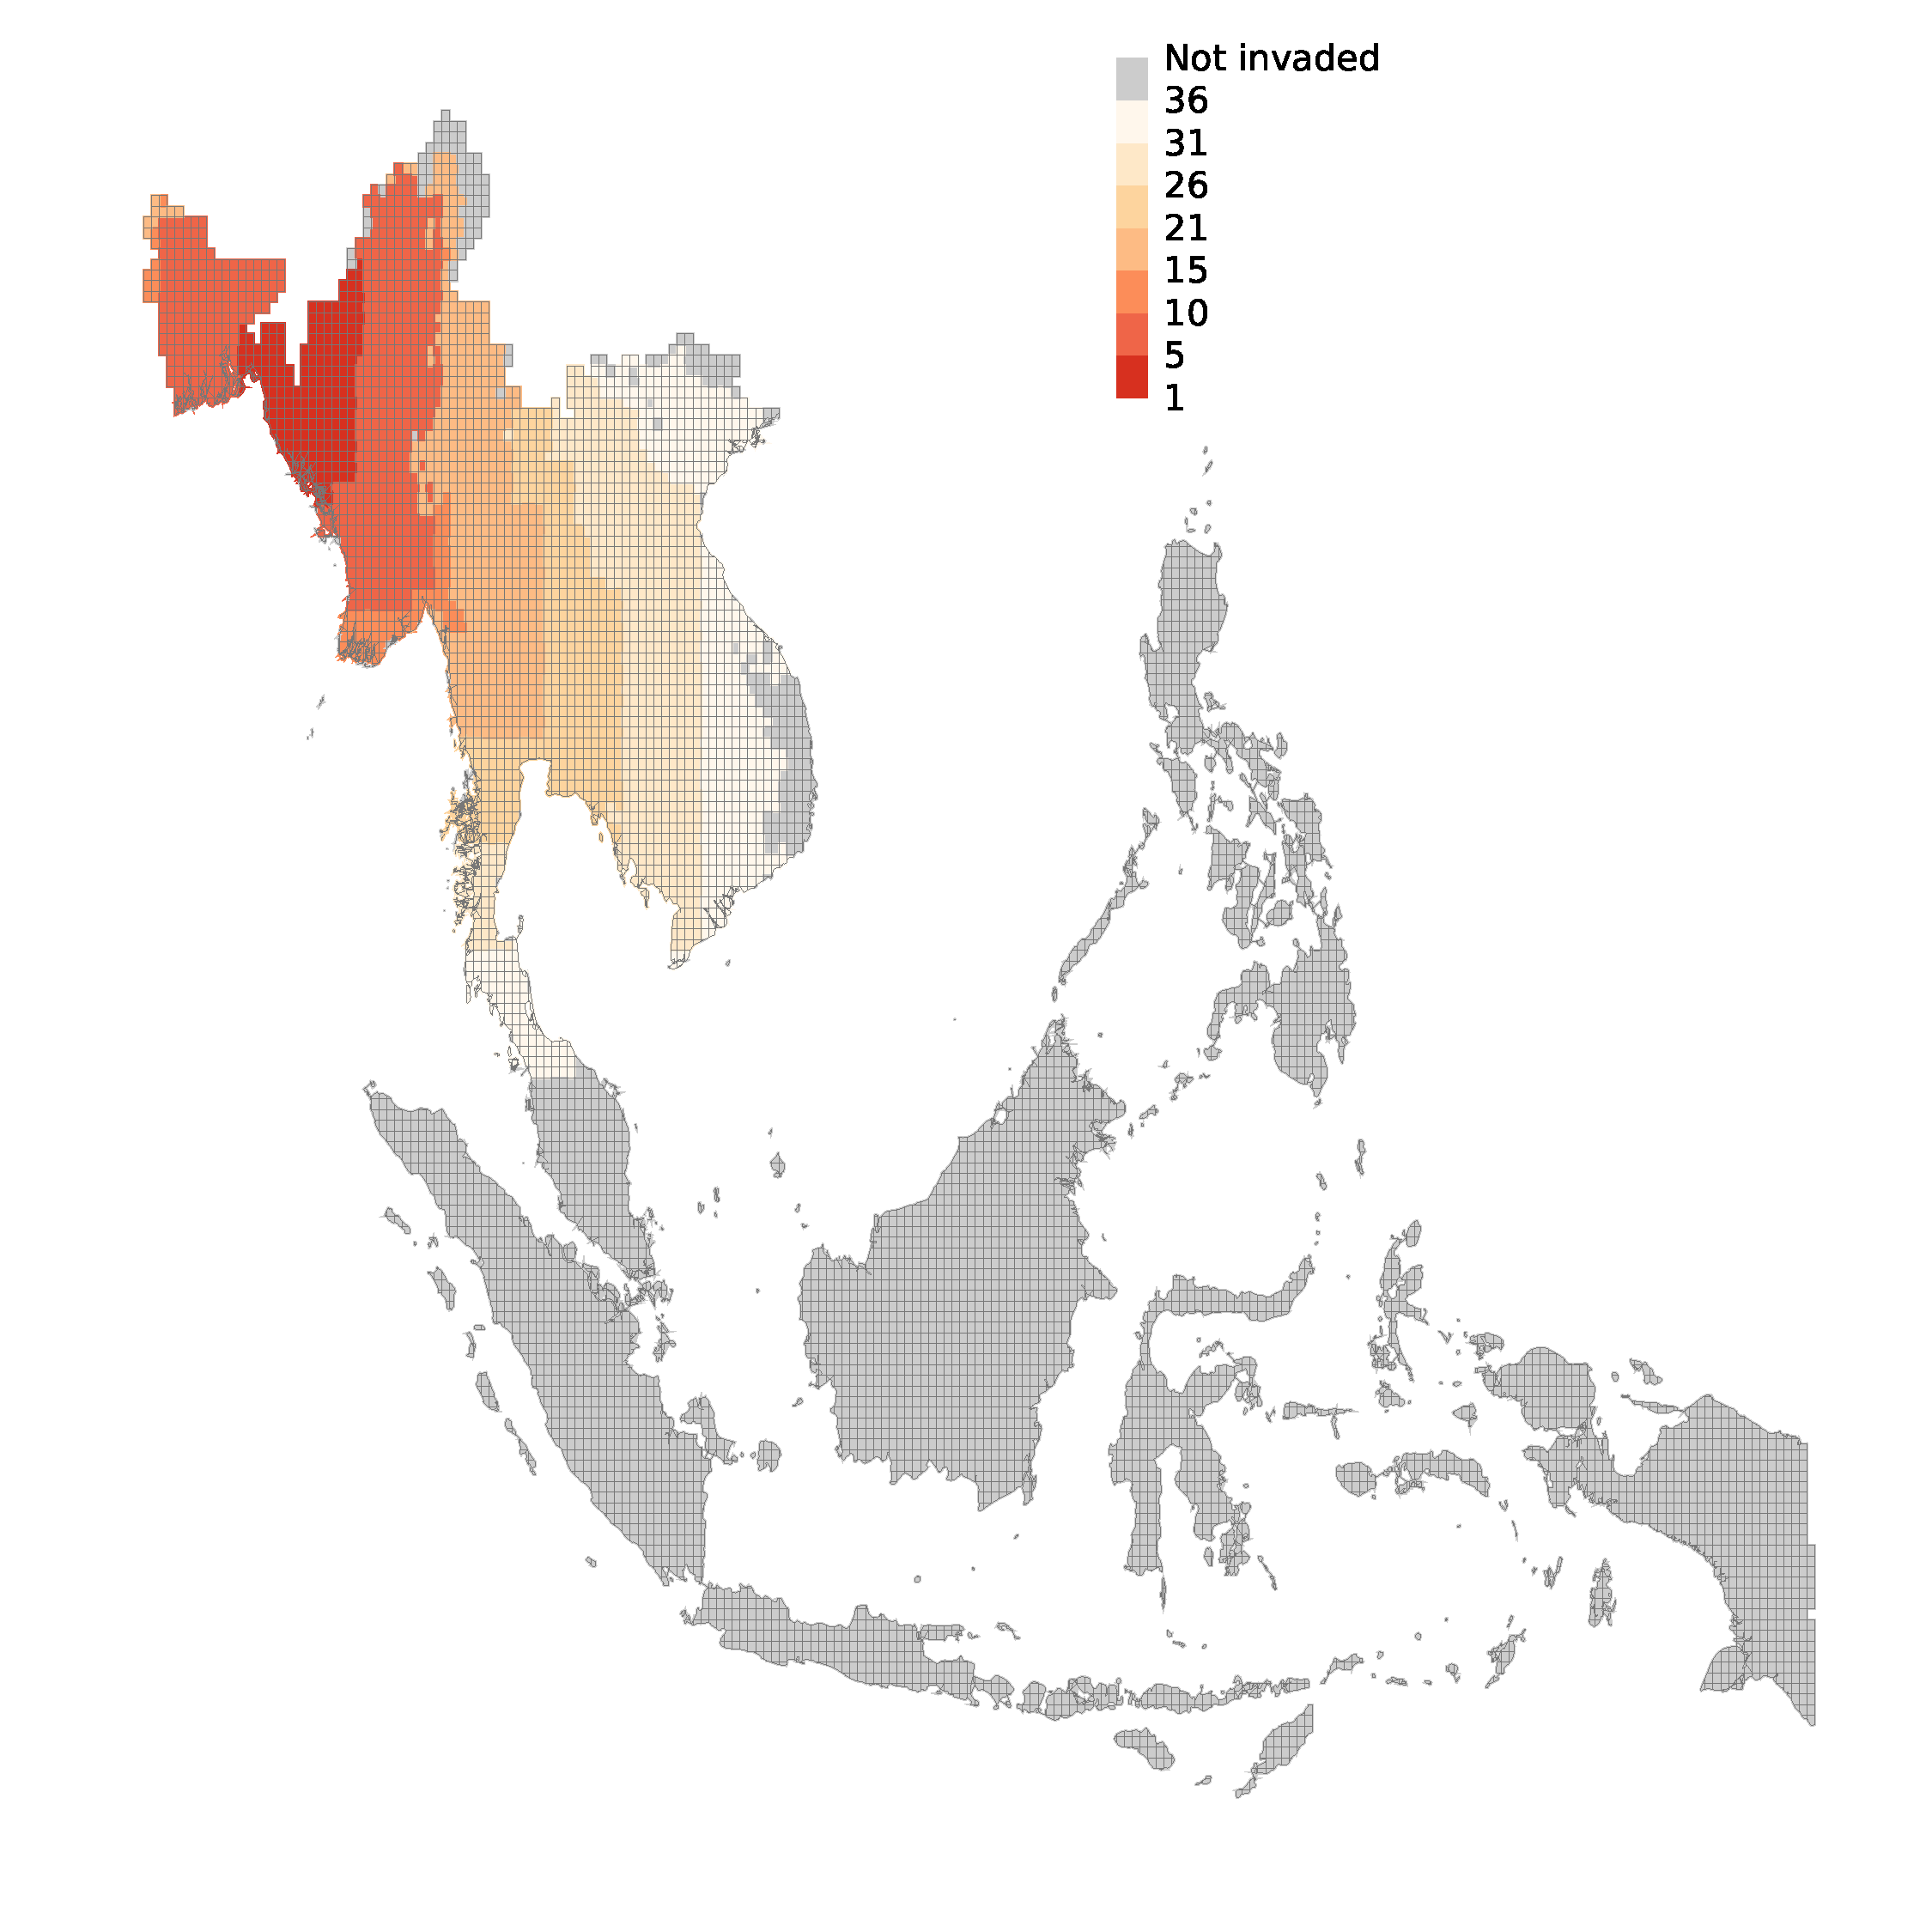
\includegraphics[width=\textwidth]{figs/plot_Myanmar2.pdf}
%% \caption{Moore neighborhood of 2, baseline model}
%% \end{subfigure}
%% \end{figure}
%

%% \begin{figure}[ht]
%%         \centering
%% \begin{subfigure}[b]{.45\textwidth}
%%         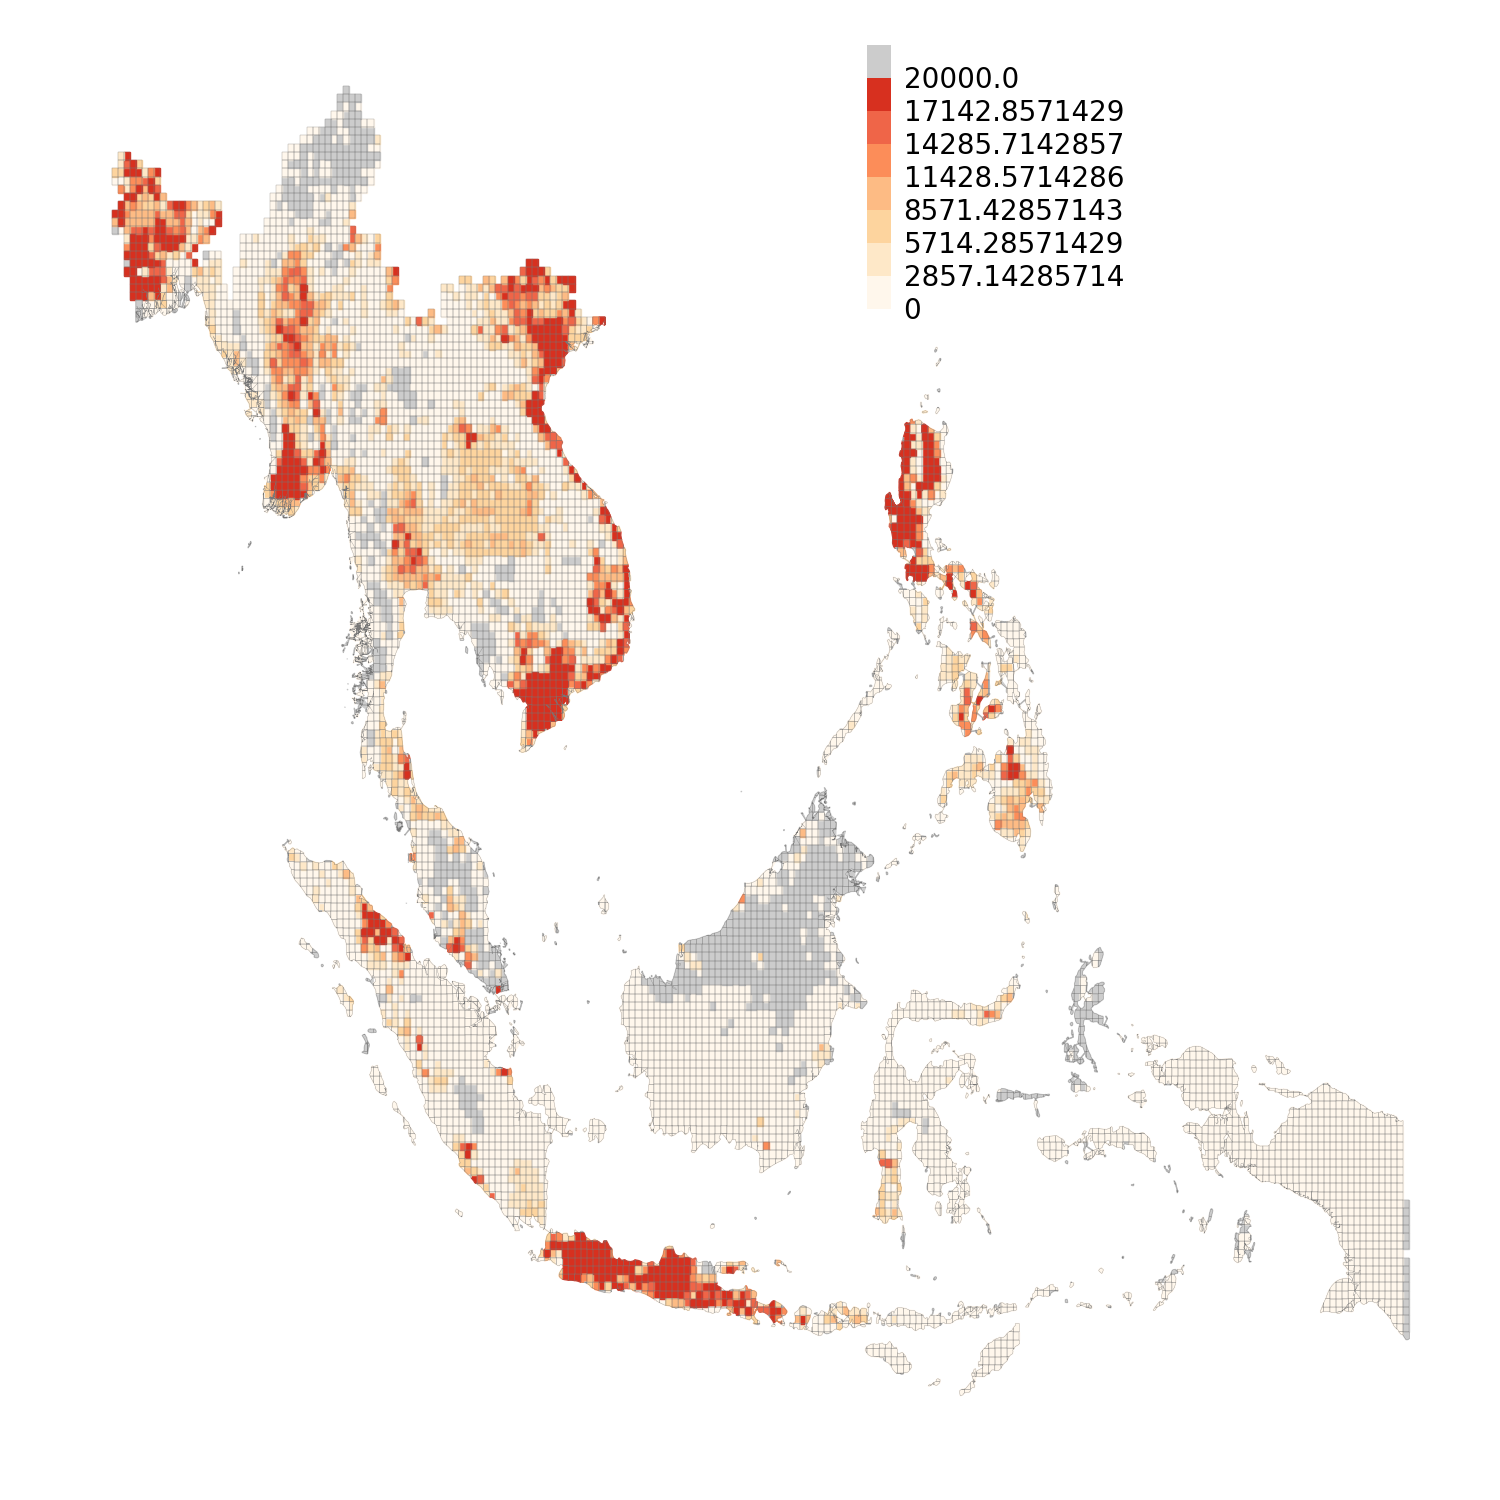
\includegraphics[width=\textwidth]{figs/mapspam_raw.png}
%%         \caption{ Mapspam Vegetable Production}
%% 
%% \end{subfigure}
%% %
%% \begin{subfigure}[b]{.45\textwidth}
%%         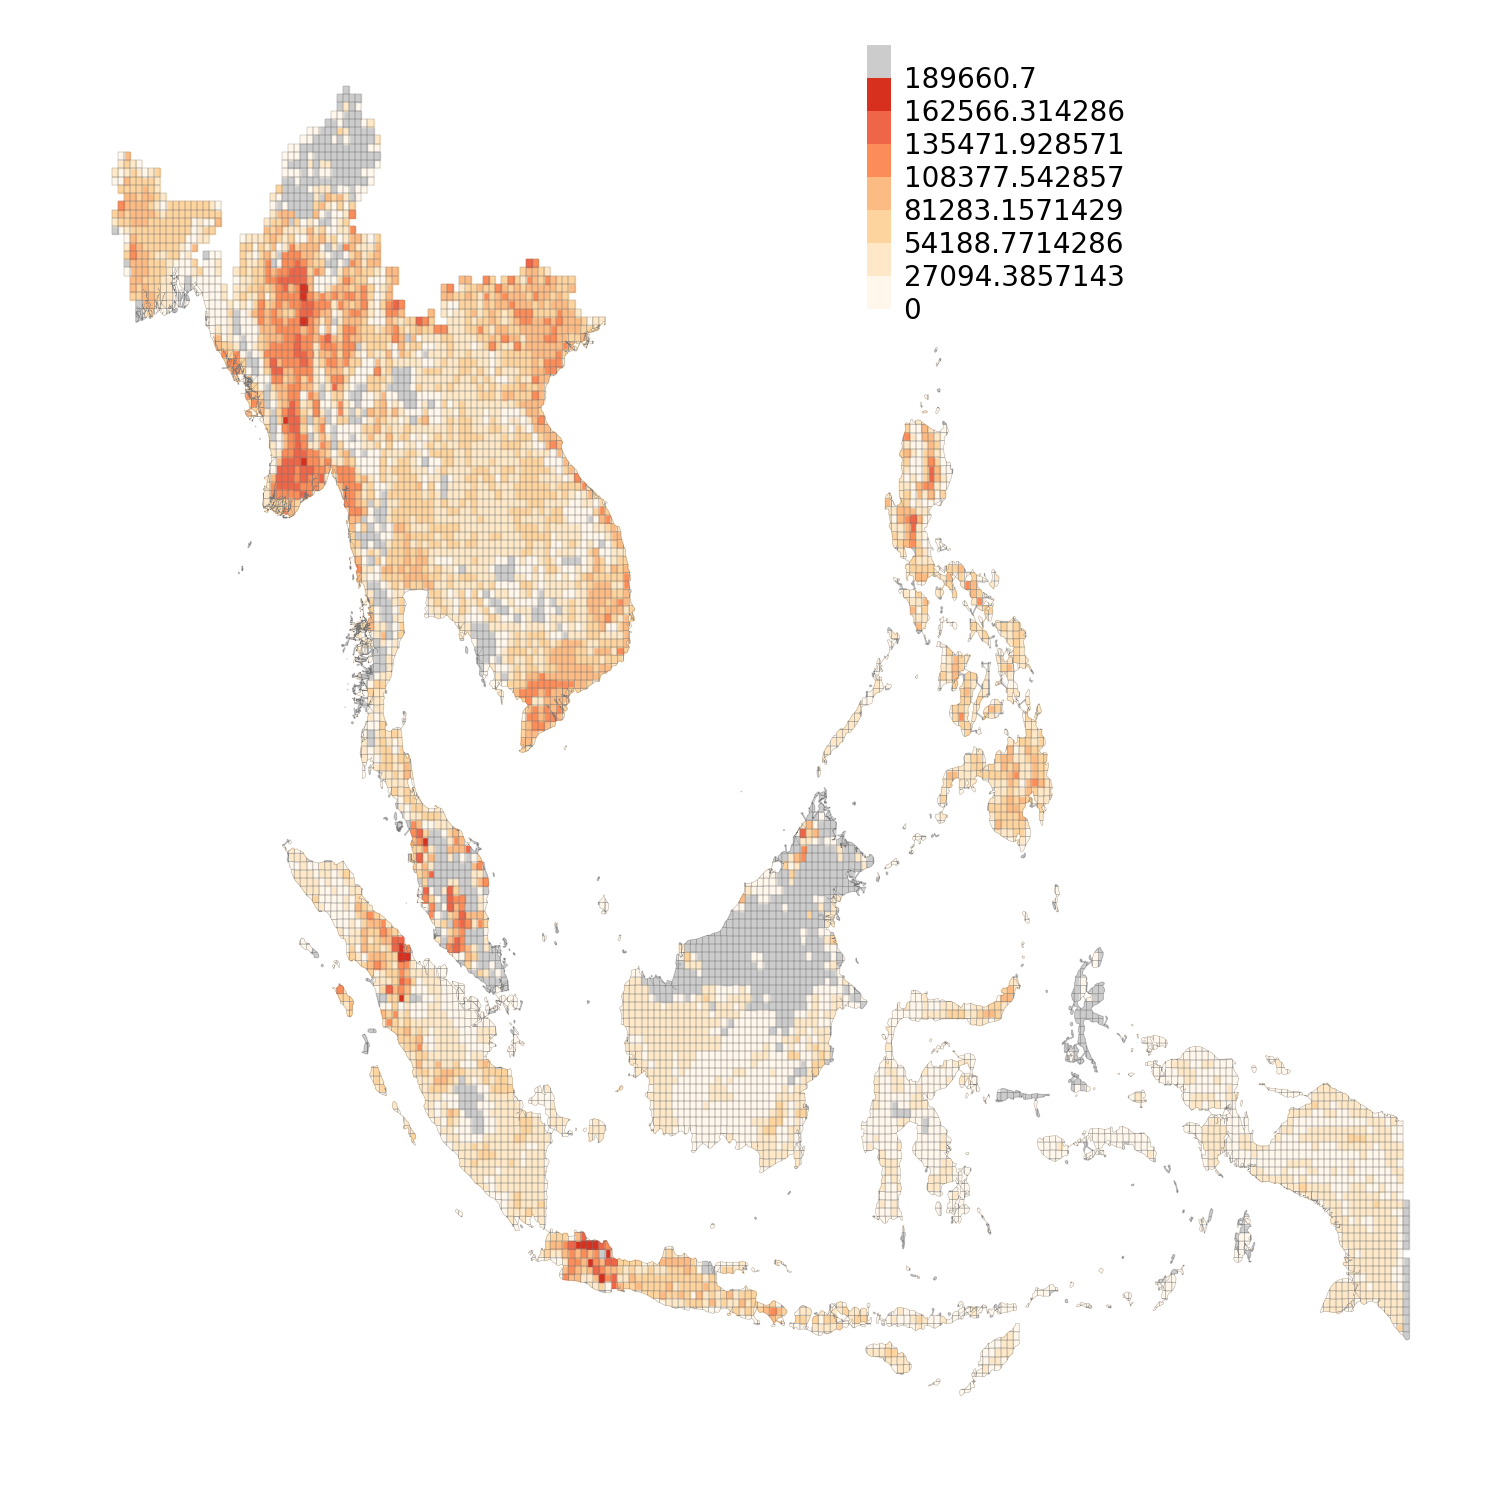
\includegraphics[width=\textwidth]{figs/mapspam_yield.png}
%%         \caption{Mapspam Vegetable Yield}
%% \end{subfigure}
%% \caption{}
%% \end{figure}
%
%% \begin{figure}[ht]
%% 
%% \begin{subfigure}[b]{.45\textwidth}
%%         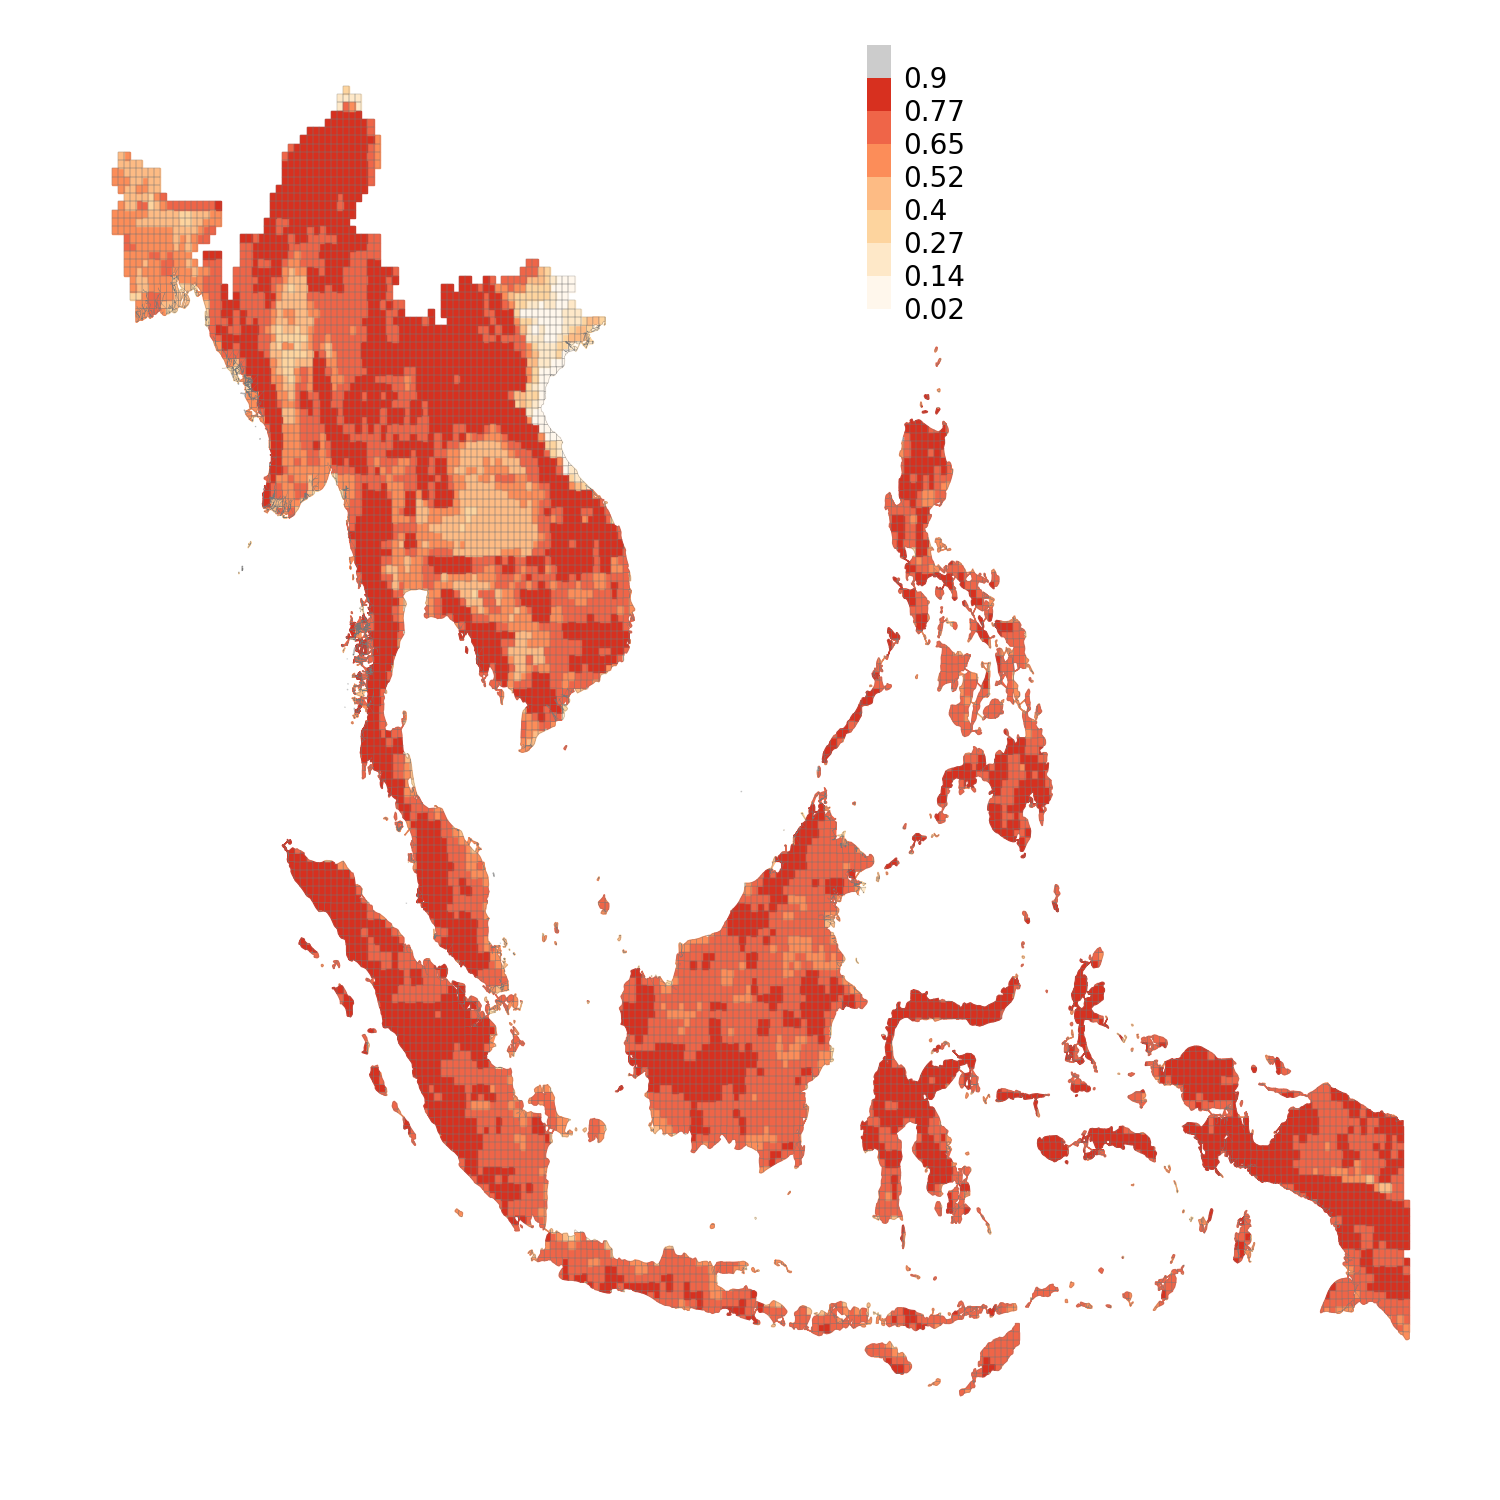
\includegraphics[width=\textwidth]{figs/heatmap_ndvi0.png}
%%         \caption{NDVI Jan.}
%% \end{subfigure}
%% %
%% \begin{subfigure}[b]{.45\textwidth}
%%         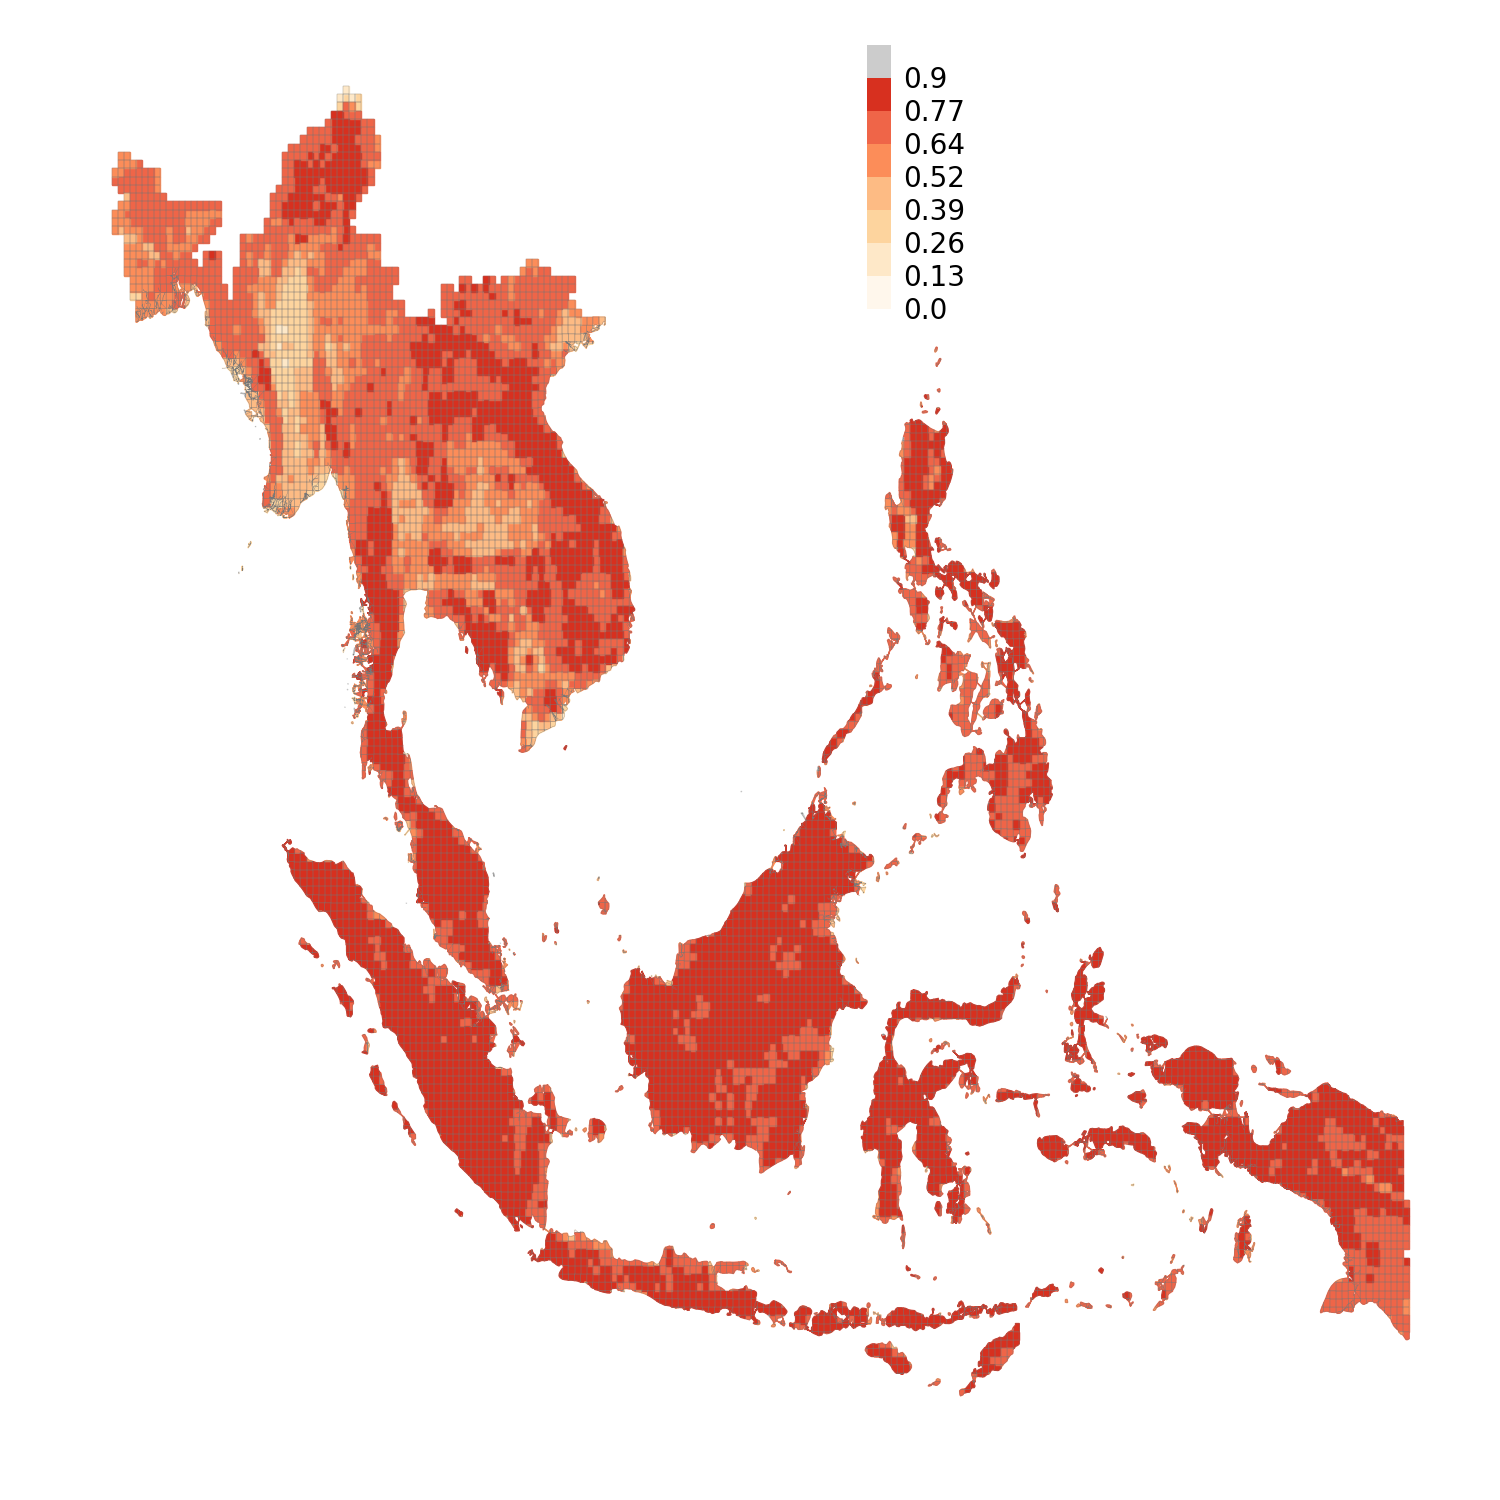
\includegraphics[width=\textwidth]{figs/heatmap_ndvi3.png}
%%         \caption{NDVI Apr.}
%% \end{subfigure}
%% %
%% \begin{subfigure}[b]{.45\textwidth}
%%         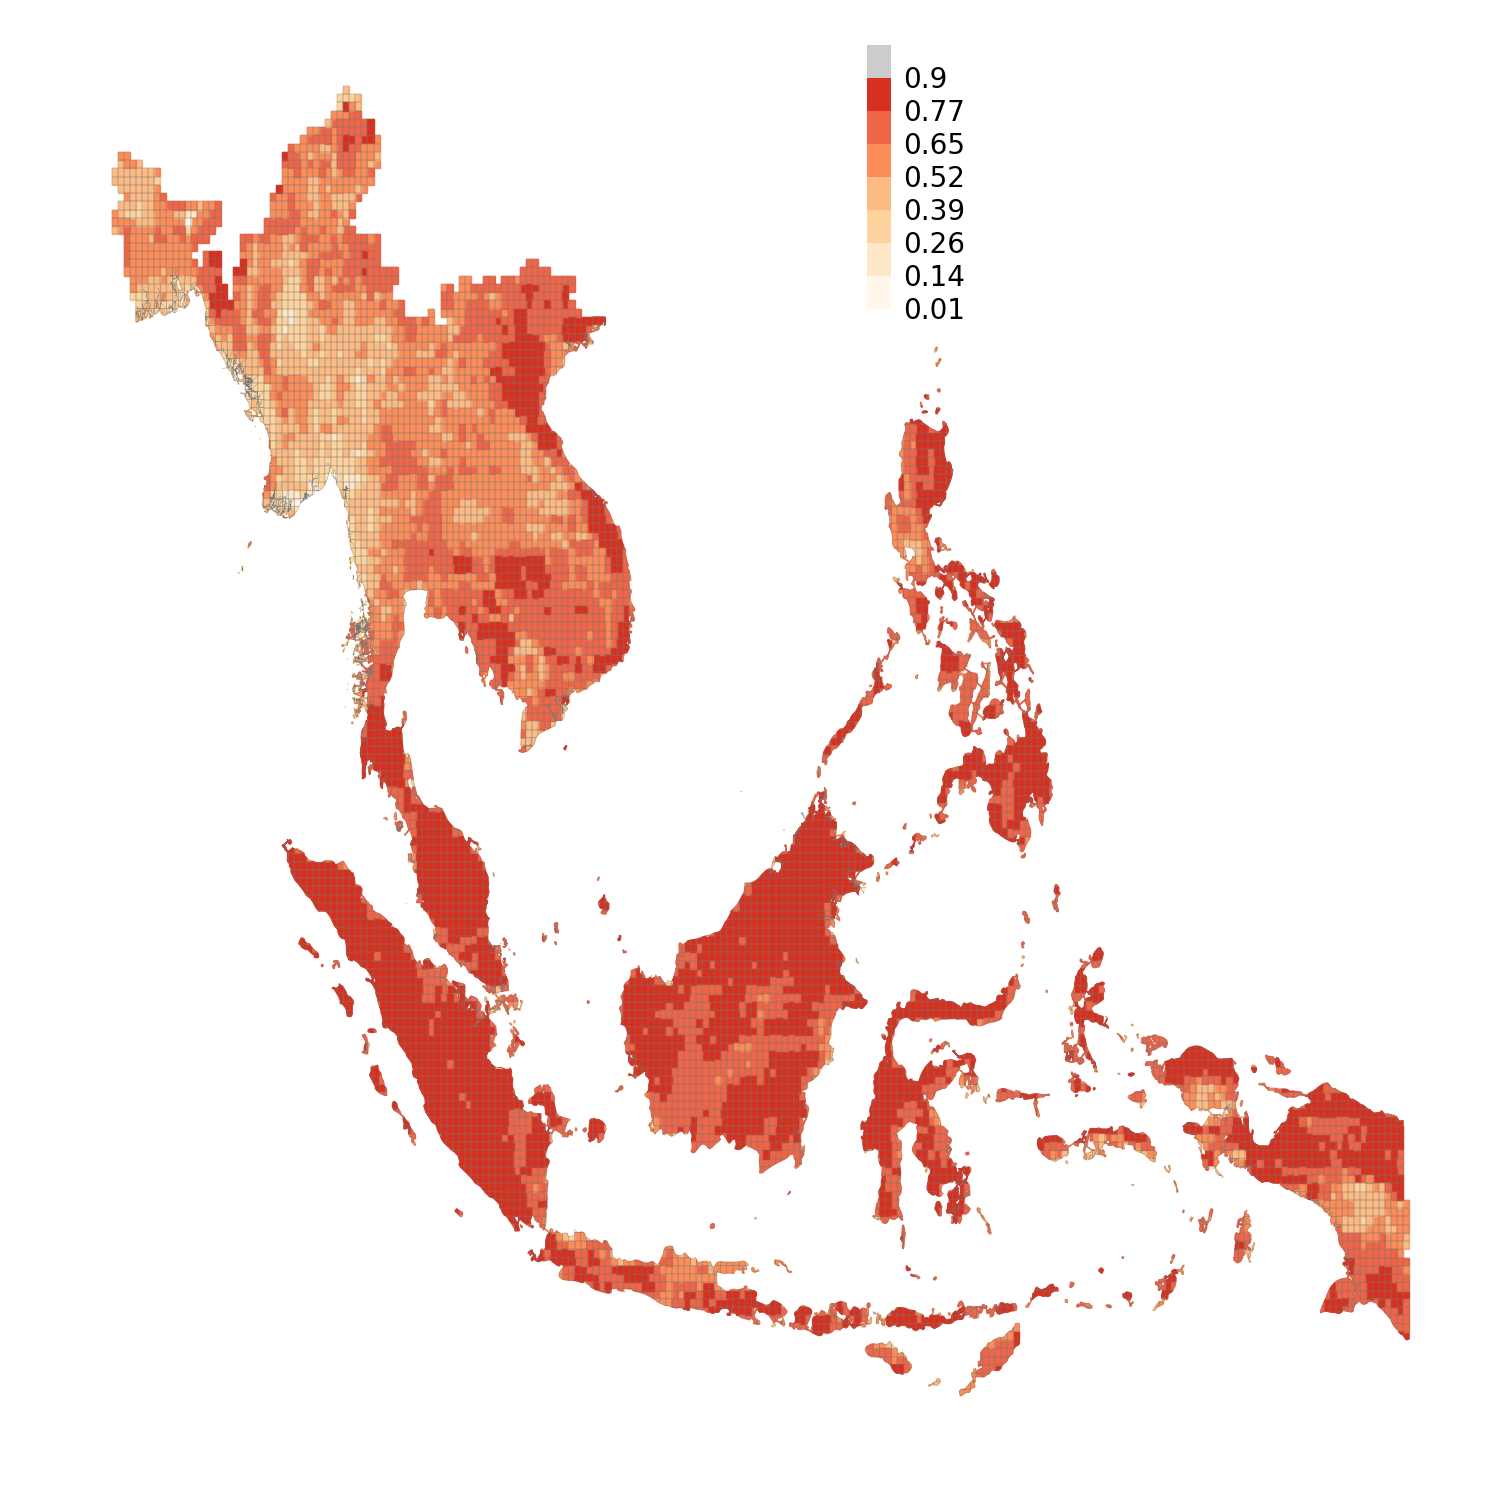
\includegraphics[width=\textwidth]{figs/heatmap_ndvi6.png}
%%         \caption{NDVI July}
%% \end{subfigure}
%% %
%% \begin{subfigure}[b]{.45\textwidth}
%%         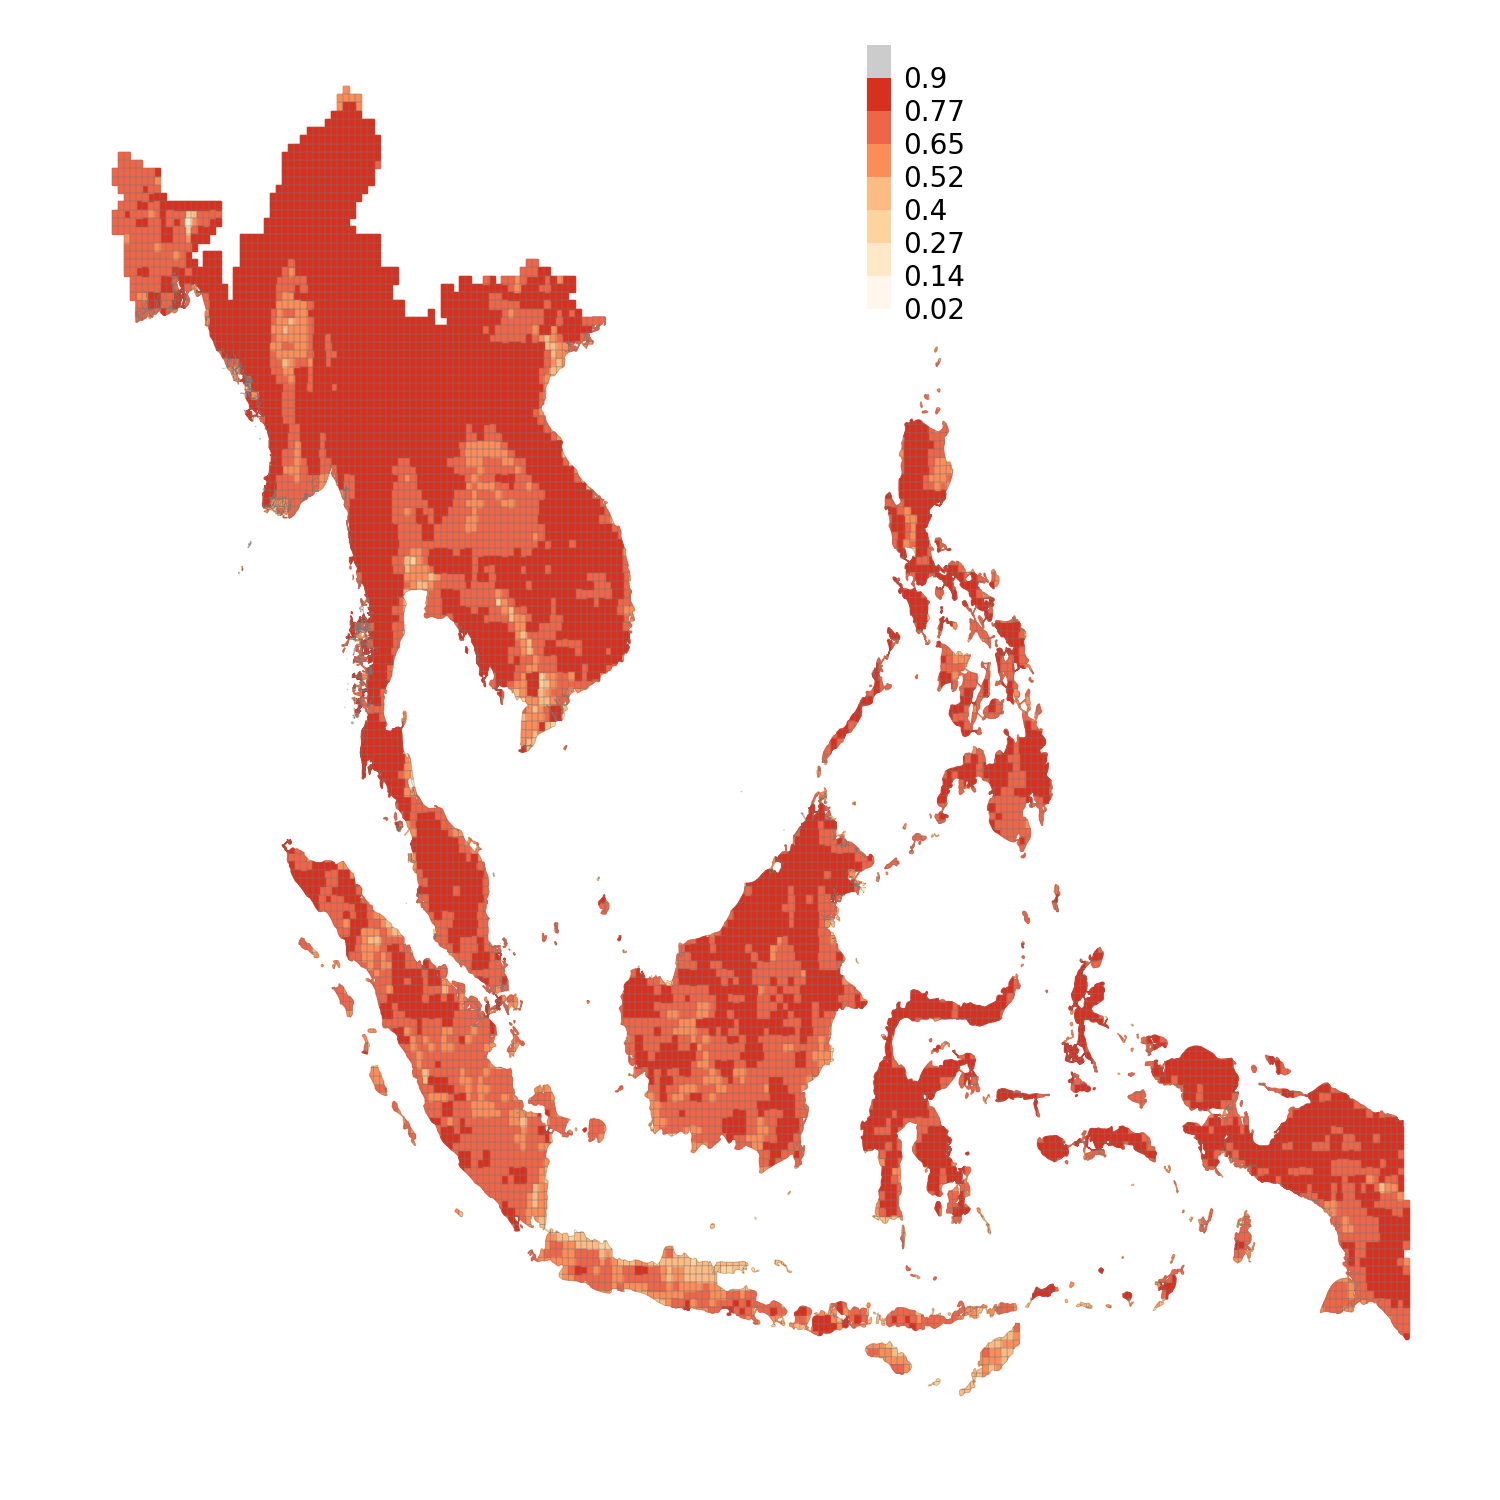
\includegraphics[width=\textwidth]{figs/heatmap_ndvi9.png}
%%         \caption{NDVI Oct.}
%% \end{subfigure}
%% 
%% \end{figure}
%
%% \begin{figure}[ht]
%% \begin{subfigure}[b]{.45\textwidth}
%%         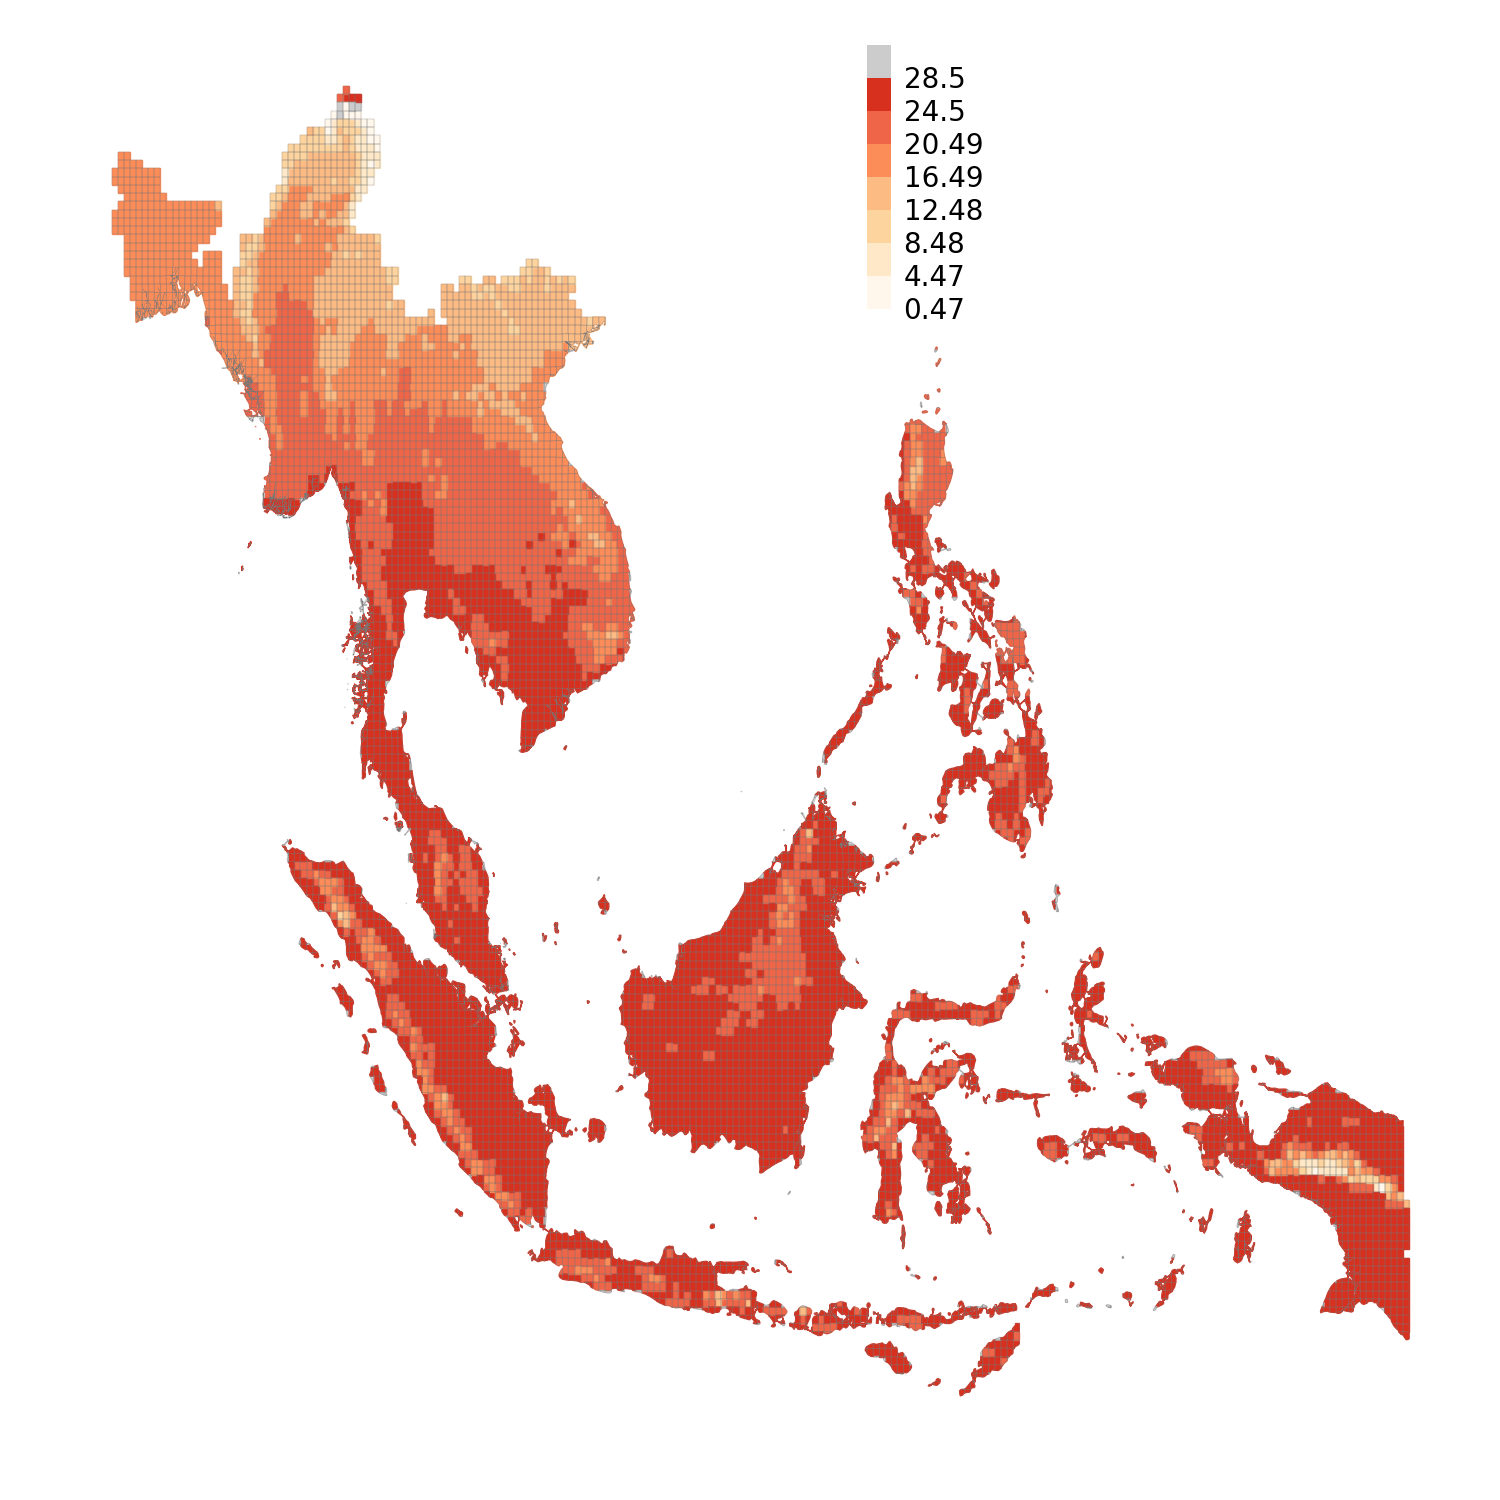
\includegraphics[width=\textwidth]{figs/heatmap_temp0.png}
%%         \caption{Temp Jan.}
%% \end{subfigure}
%% %
%% \begin{subfigure}[b]{.45\textwidth}
%%         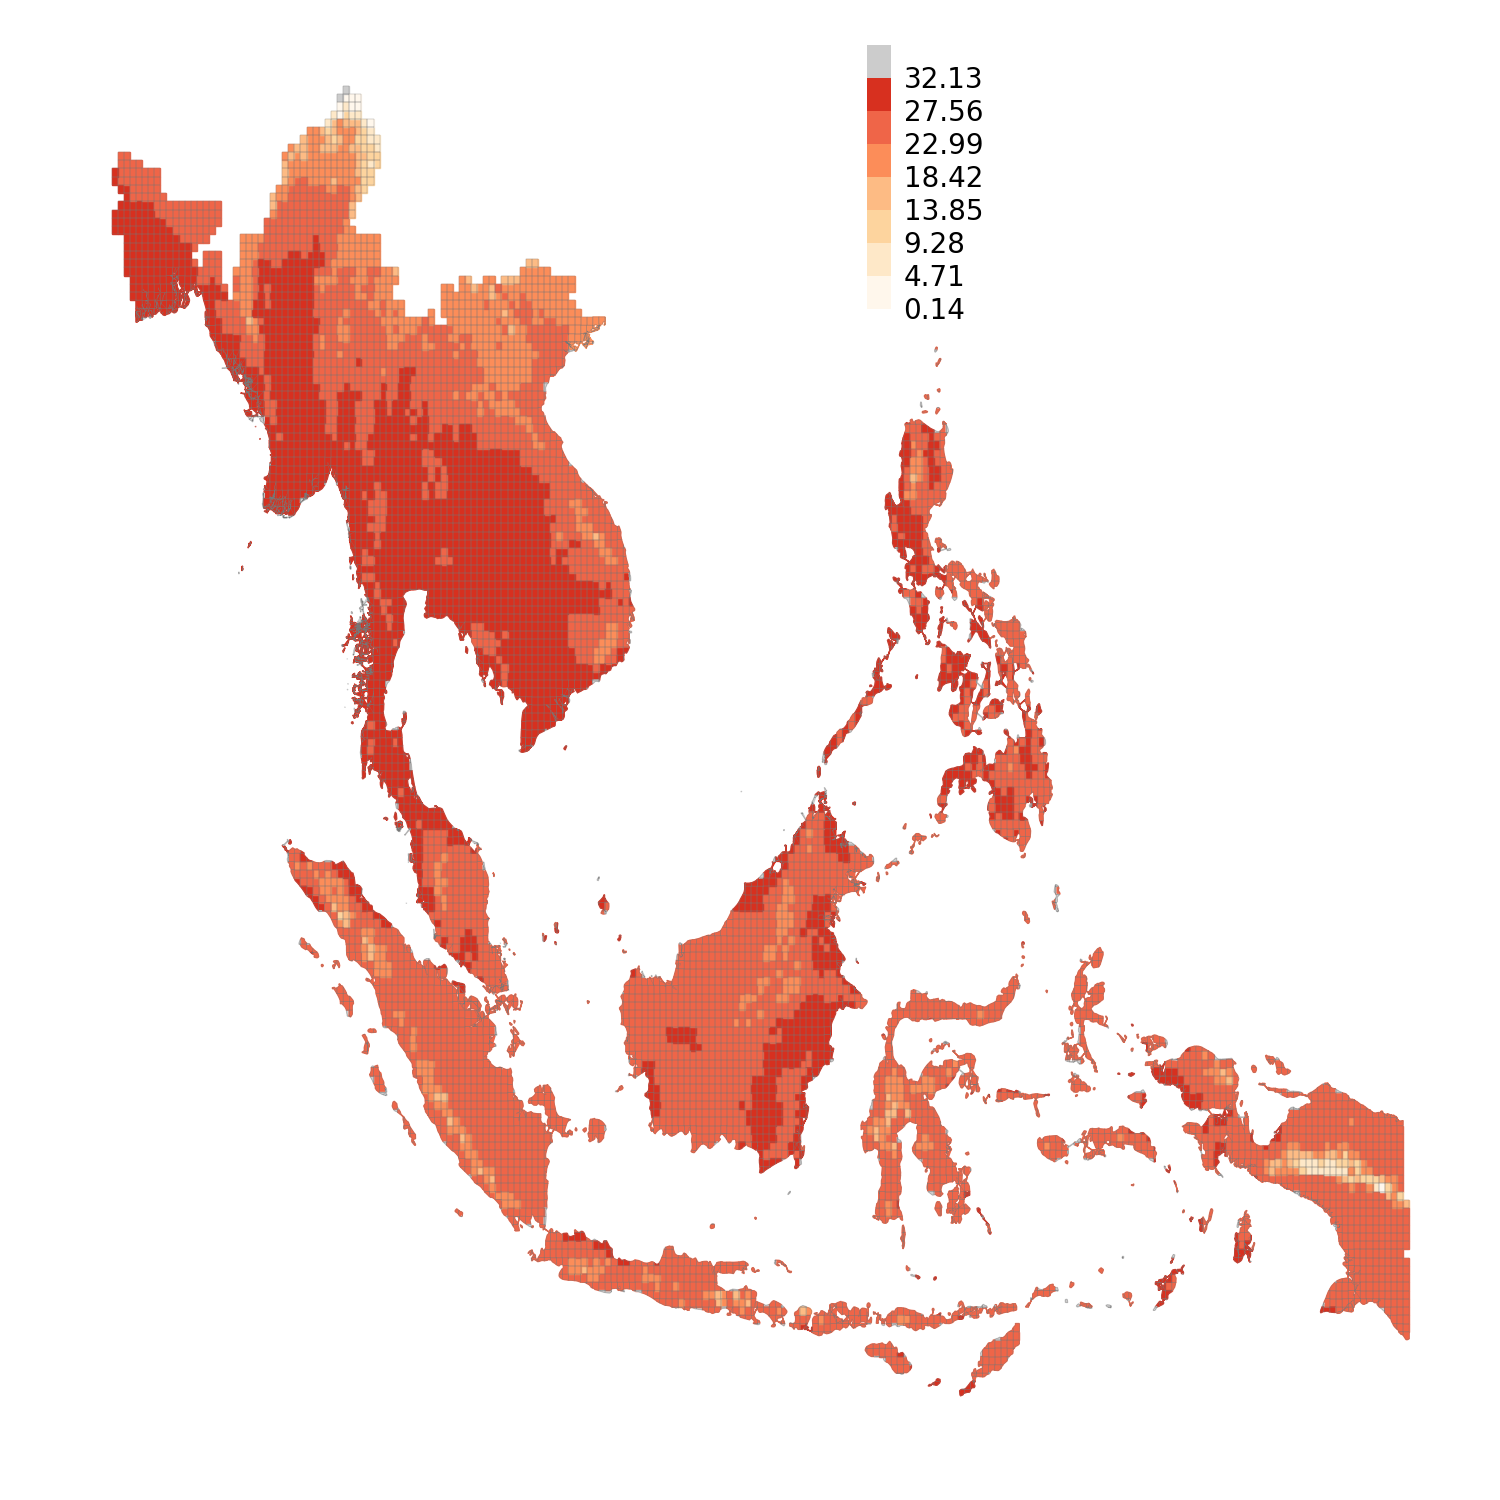
\includegraphics[width=\textwidth]{figs/heatmap_temp3.png}
%%         \caption{Temp Apr.}
%% \end{subfigure}
%% %
%% \begin{subfigure}[b]{.45\textwidth}
%%         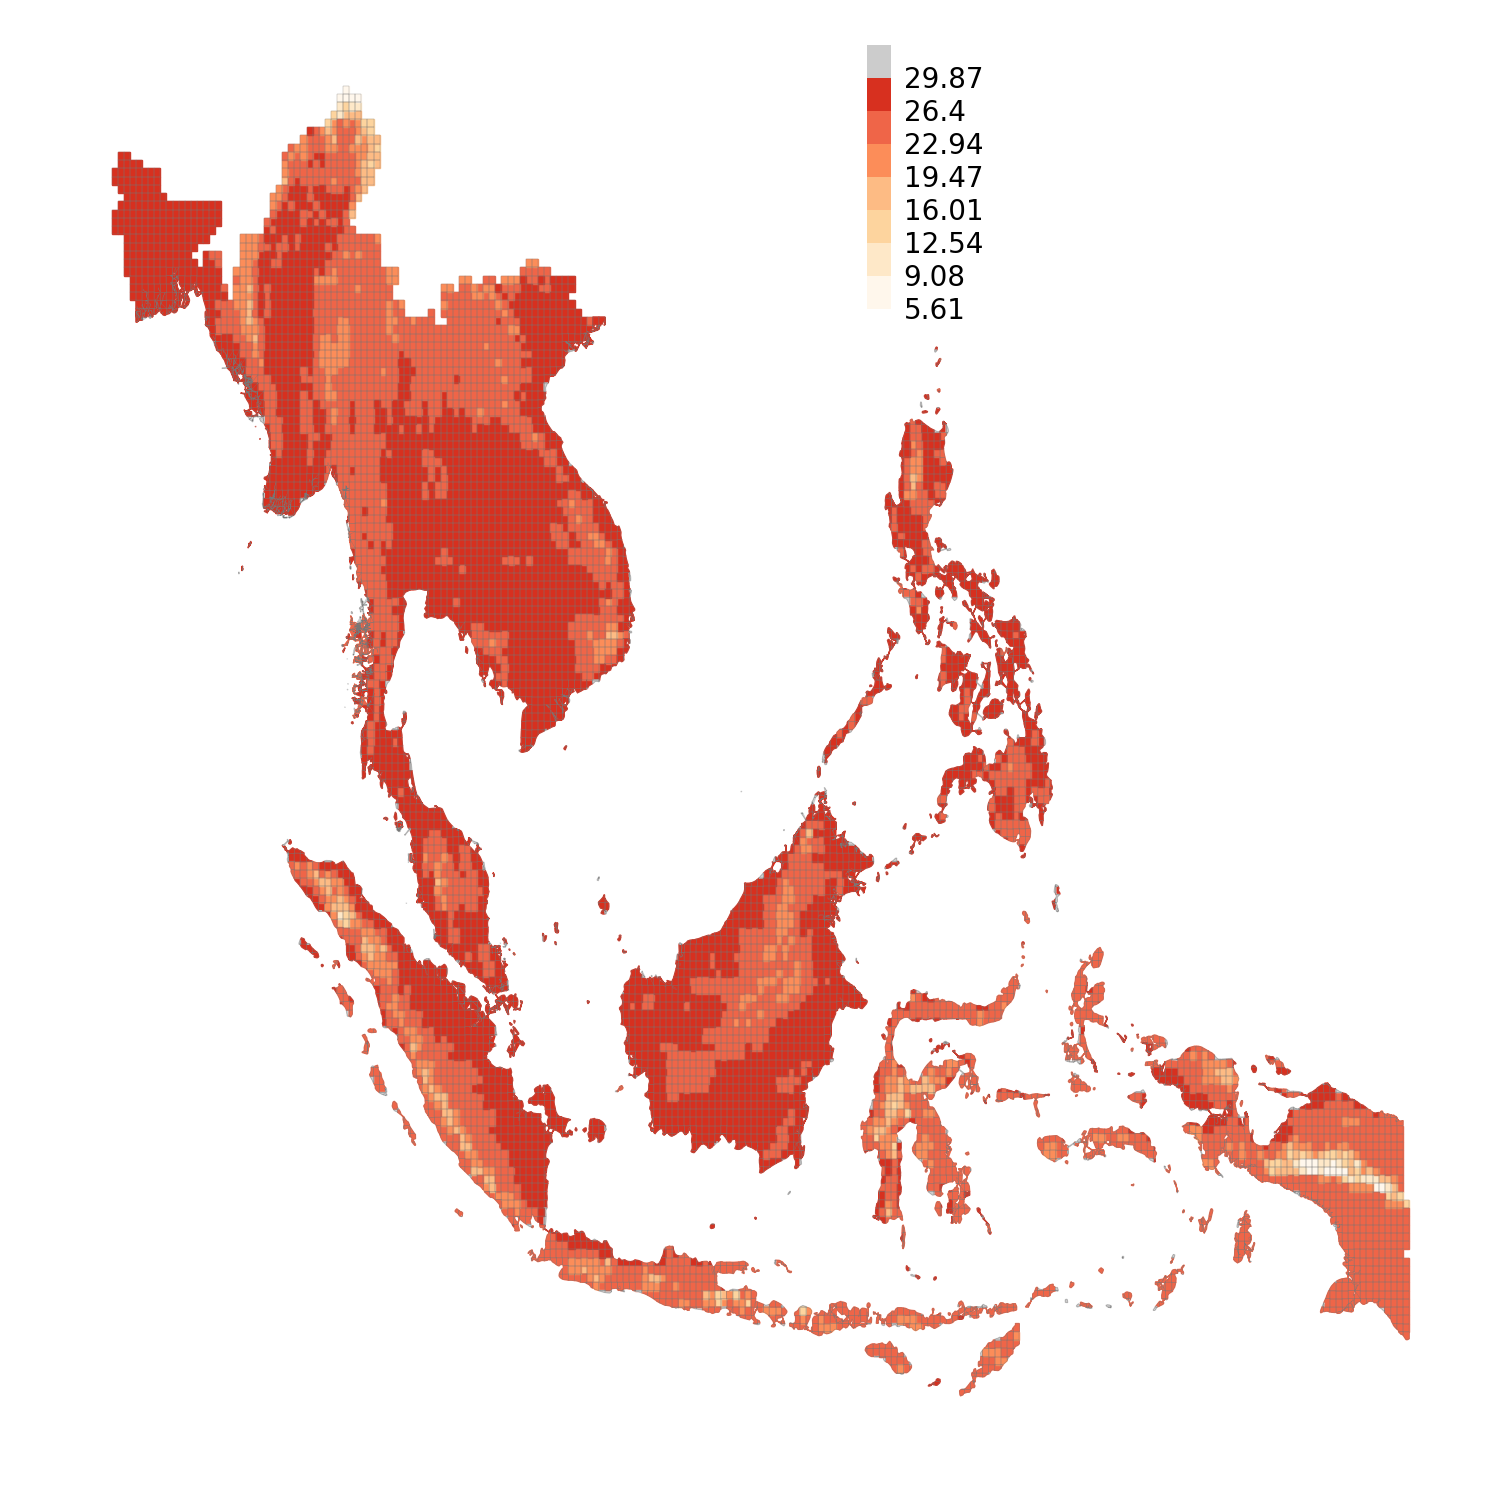
\includegraphics[width=\textwidth]{figs/heatmap_temp6.png}
%%         \caption{Temp July}
%% \end{subfigure}
%% %
%% \begin{subfigure}[b]{.45\textwidth}
%%         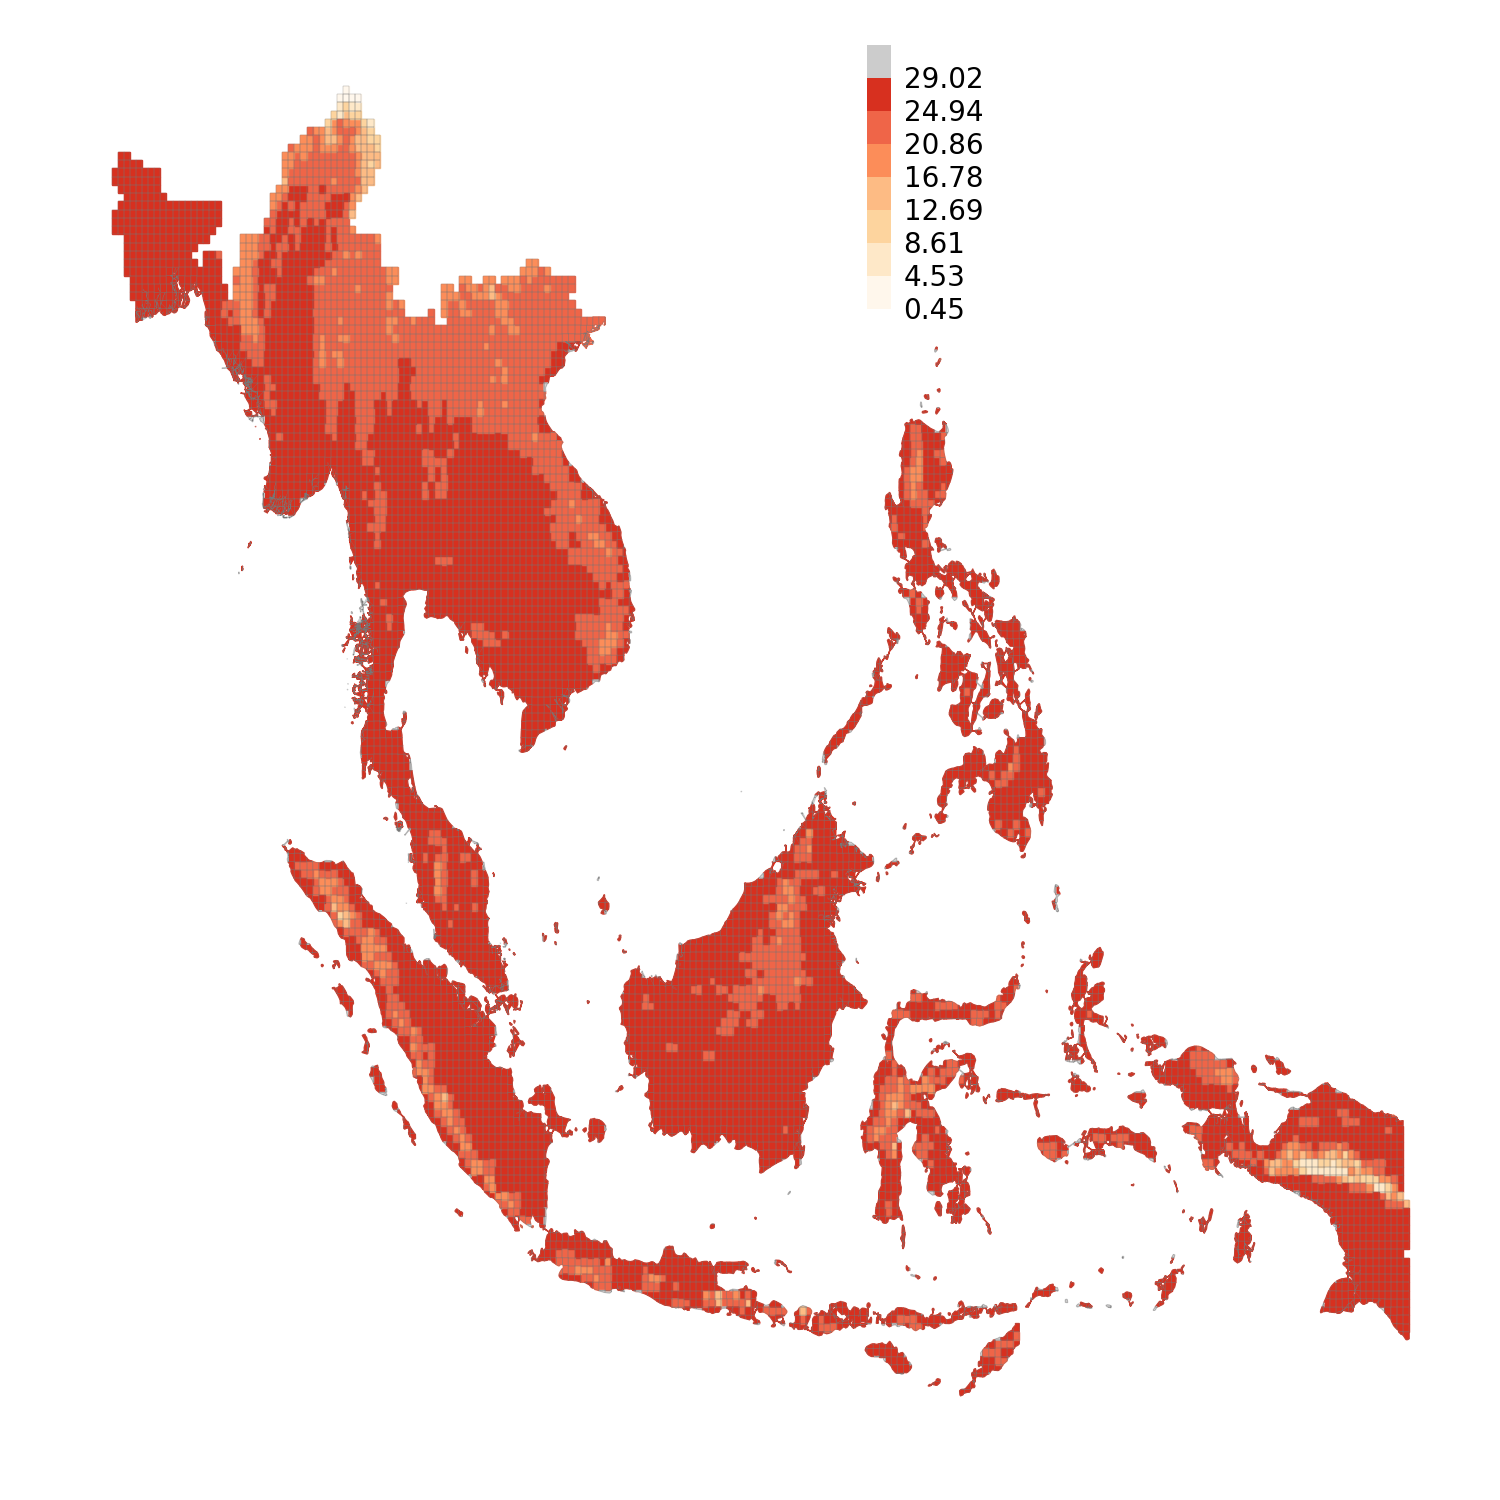
\includegraphics[width=\textwidth]{figs/heatmap_temp9.png}
%%         \caption{Temp Oct.}
%% \end{subfigure}
%% \caption{Data Plots}
%% \end{figure}
%% 
%%
 
%% \begin{figure}[ht]
%%     \centering
%% \begin{subfigure}[b]{.32\textwidth}
%%     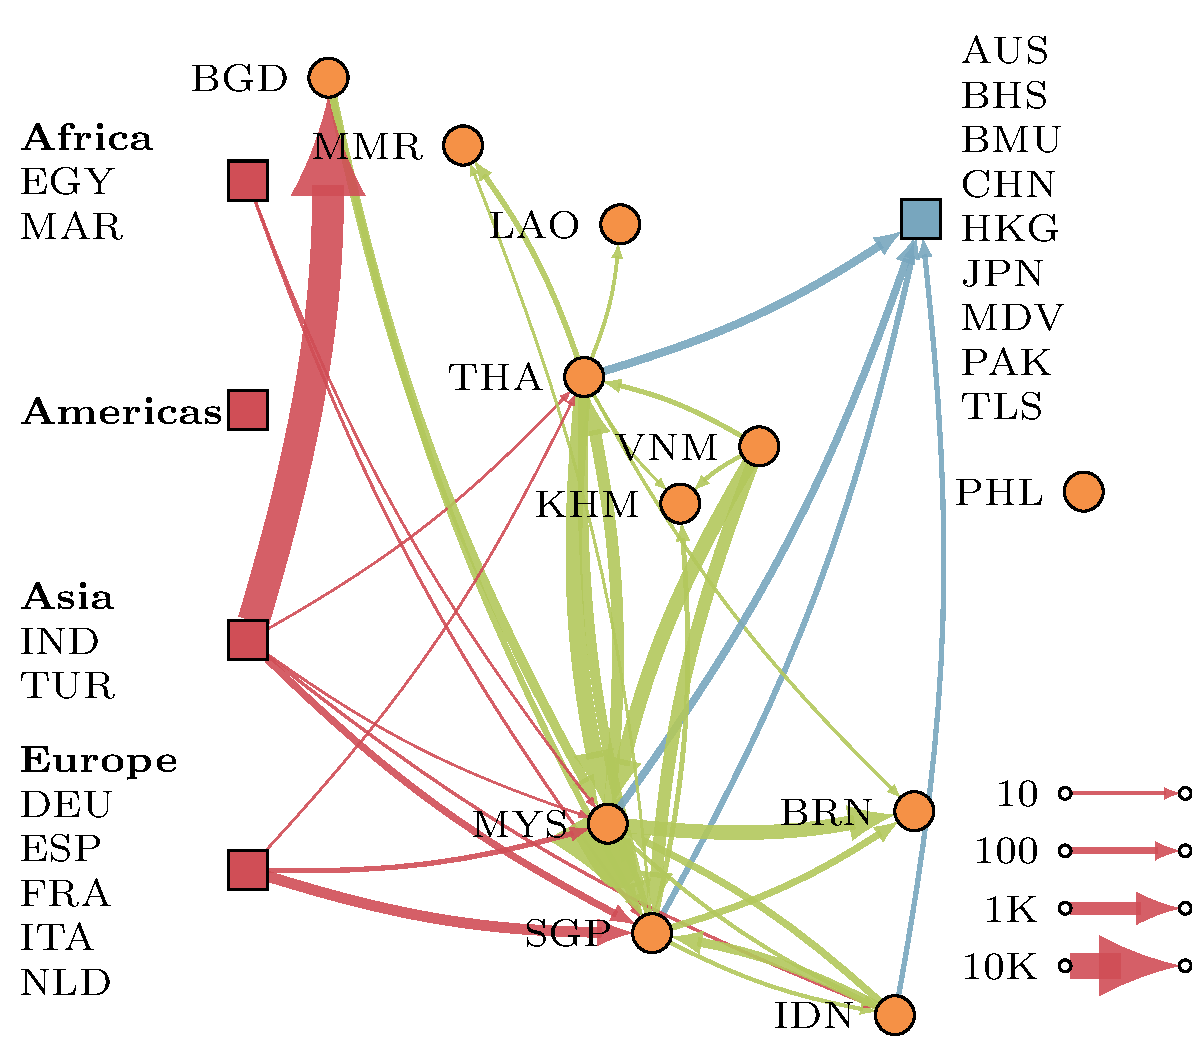
\includegraphics[width=\textwidth]{../international_trade/results/network_plots/sea_2013_tomato.pdf}
%%     \caption{Tomato}
%% \end{subfigure}
%% %%
%% \begin{subfigure}[b]{.32\textwidth}
%%     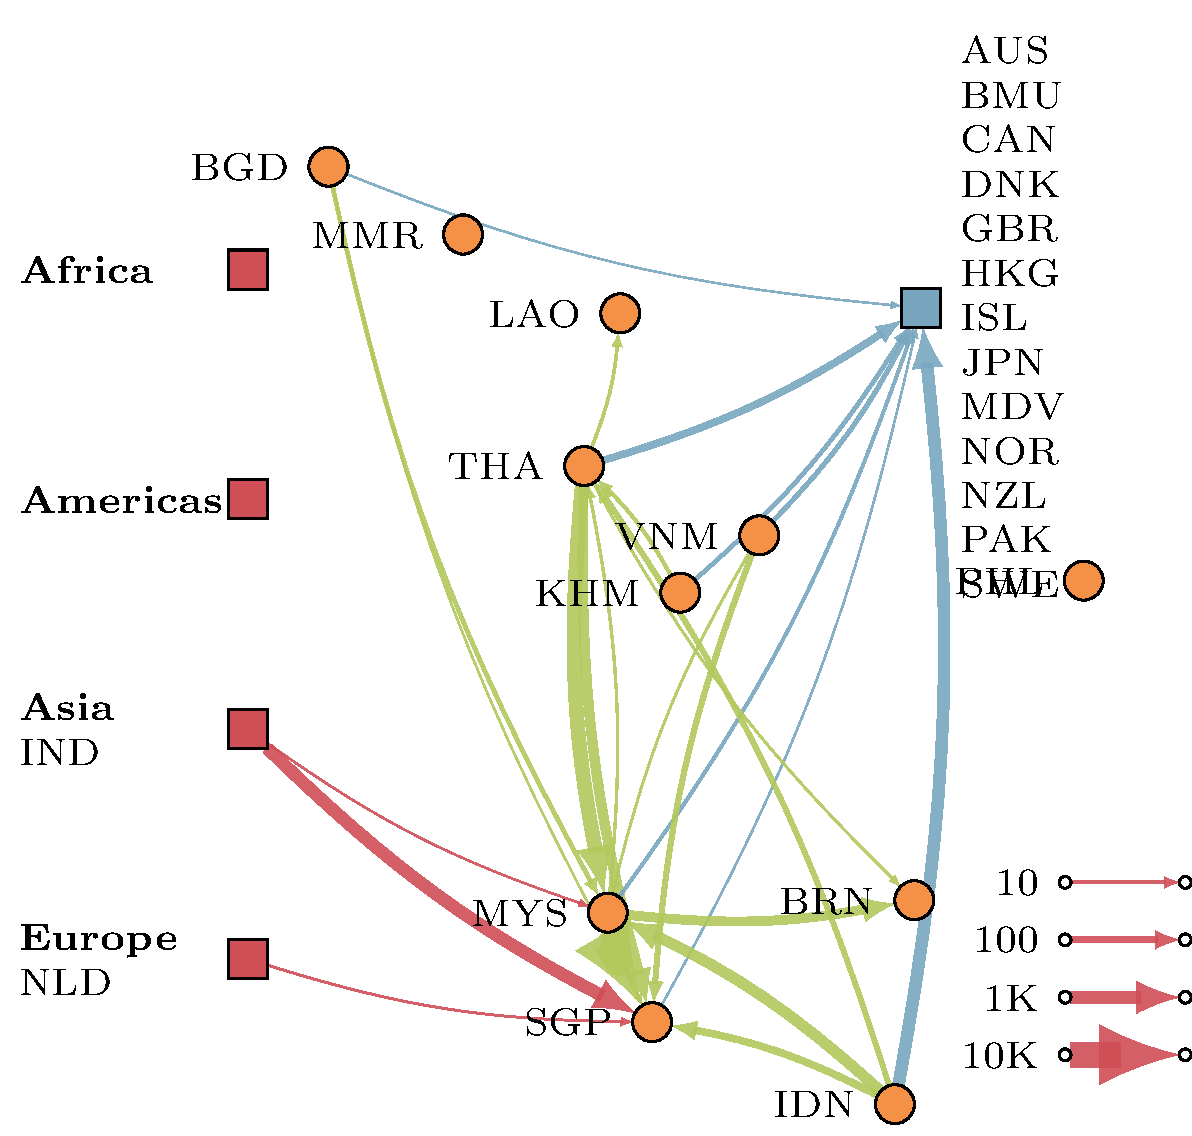
\includegraphics[width=\textwidth]{../international_trade/results/network_plots/sea_2013_eggplant.pdf}
%%     \caption{Eggplants}
%% \end{subfigure}
%%     %%
%% \begin{subfigure}[b]{.45\textwidth}
%%     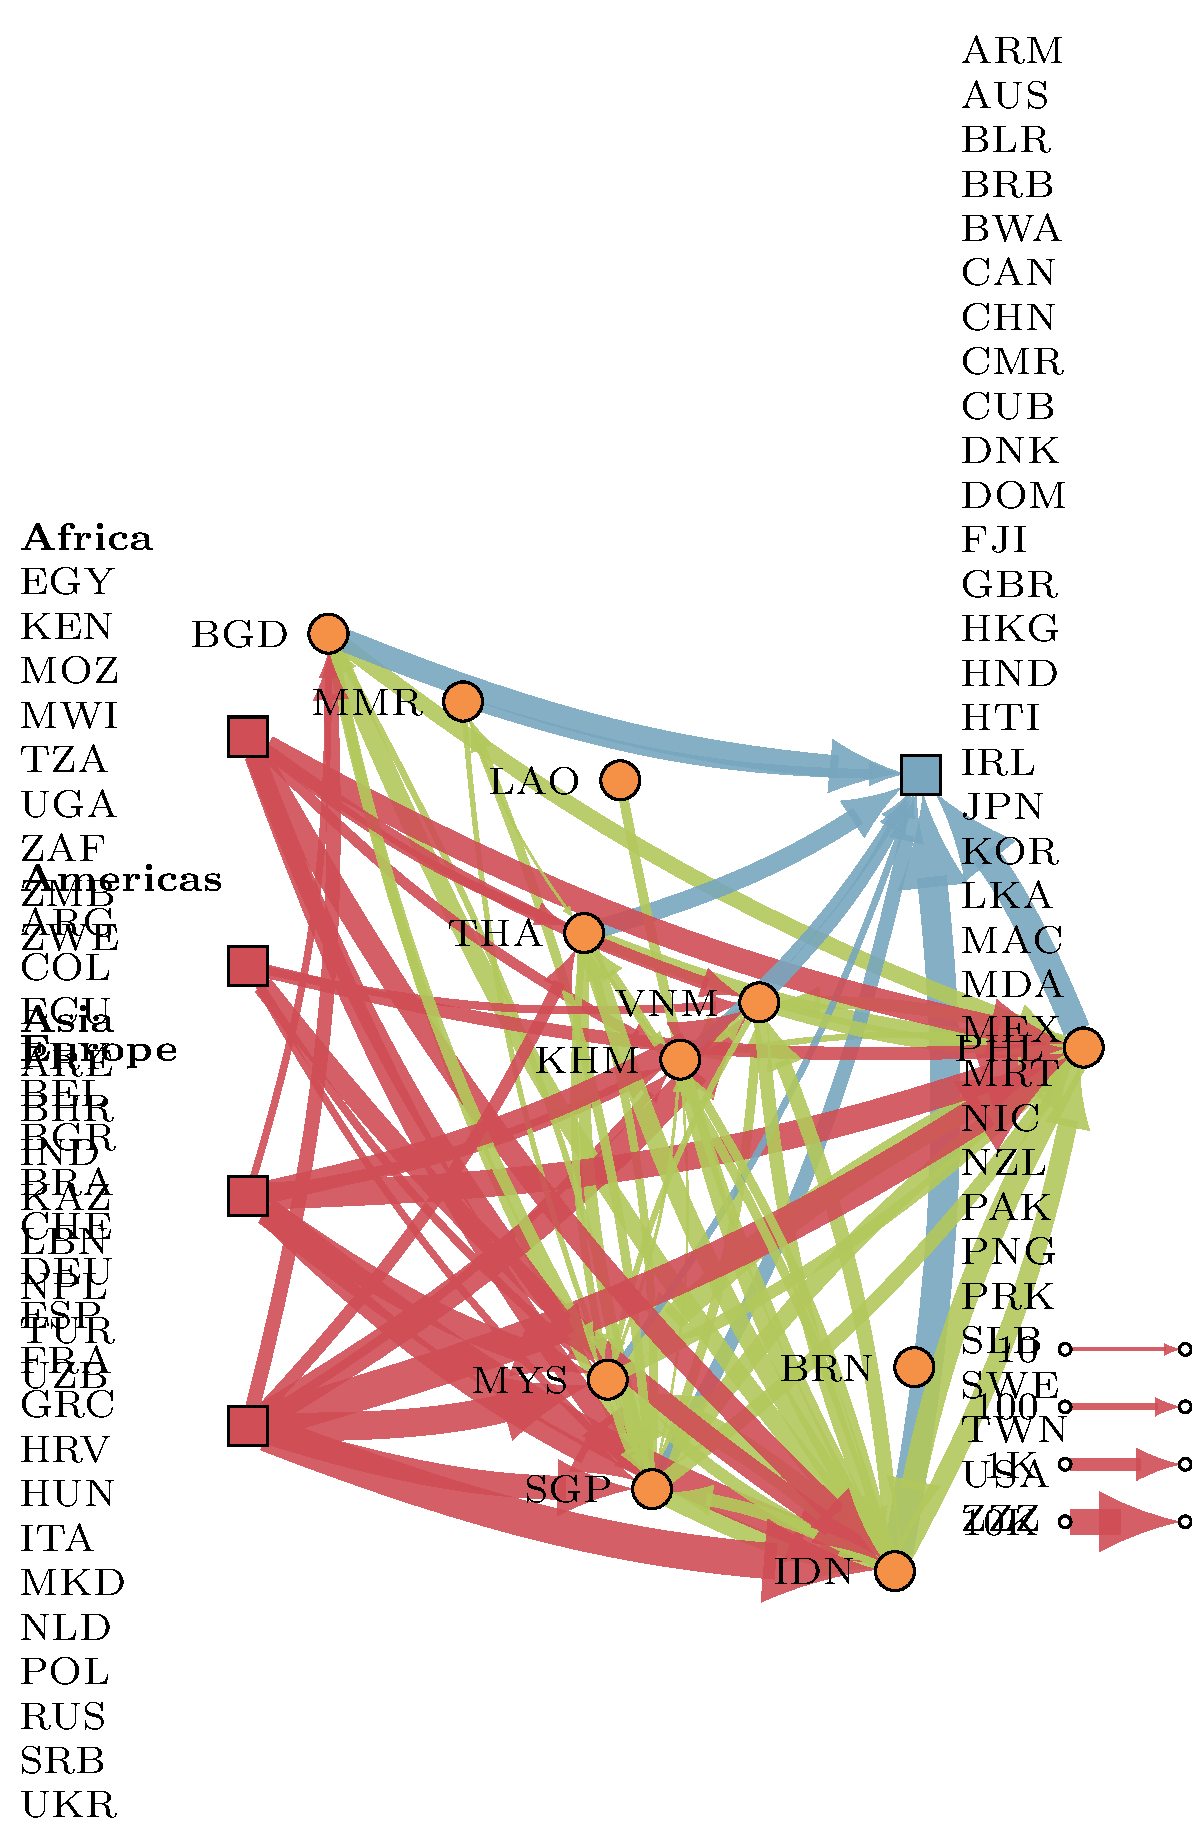
\includegraphics[width=\textwidth]{../international_trade/results/network_plots/sea_2013_tobacco.pdf}
%%     \caption{Tobacco 2013}
%% \end{subfigure}
    %%
%% \begin{subfigure}[b]{.45\textwidth}
%%     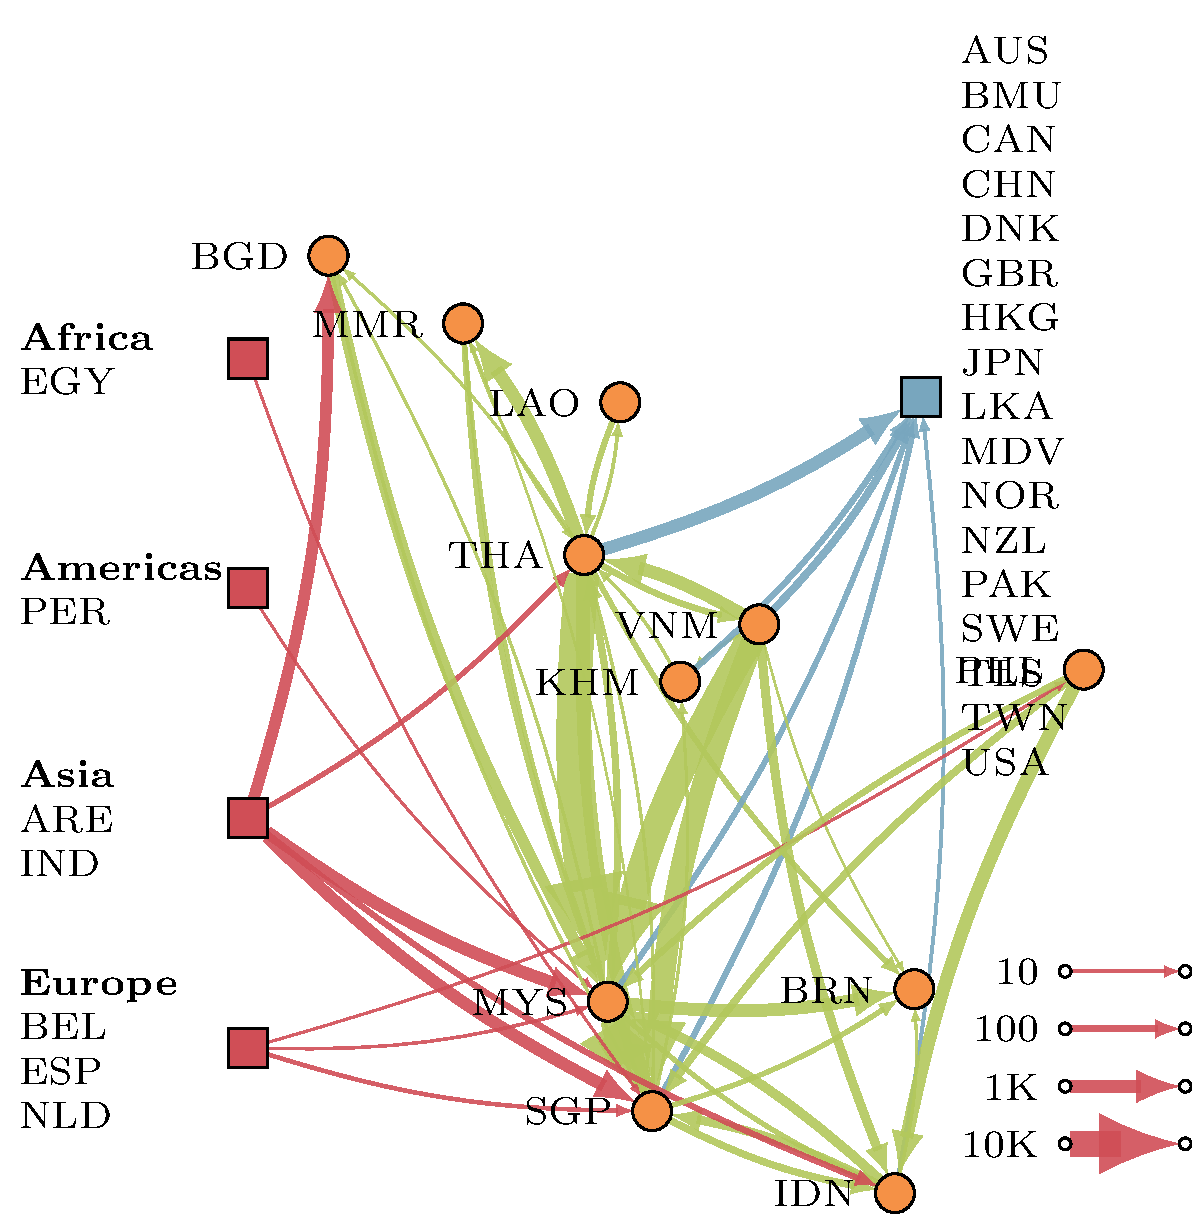
\includegraphics[width=\textwidth]{../international_trade/results/network_plots/sea_2013_pepper.pdf}
%%     \caption{Peppers 2013}
%% \end{subfigure}
    %%
%% \begin{subfigure}[b]{.32\textwidth}
%%     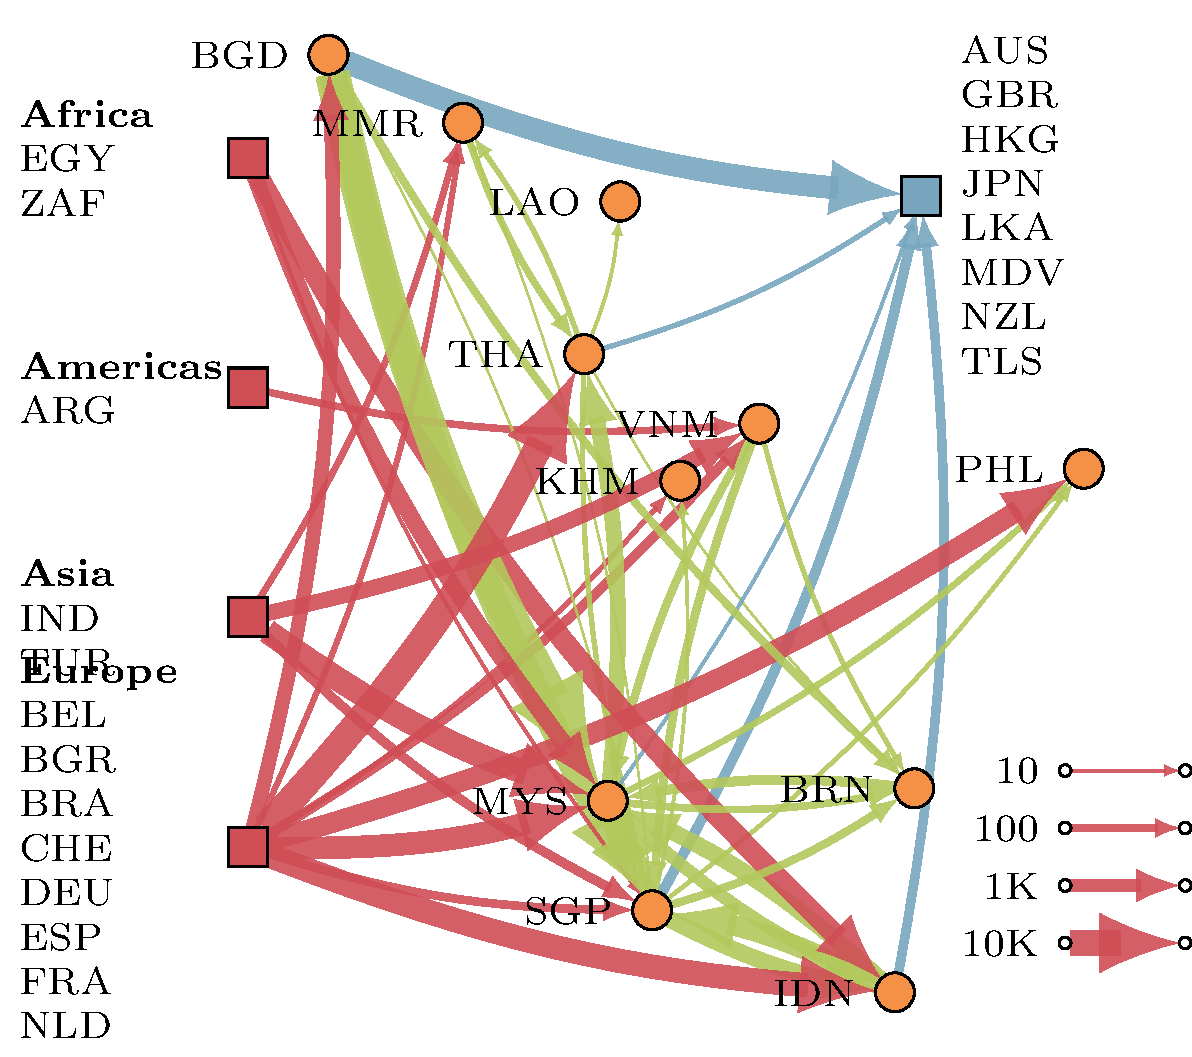
\includegraphics[width=\textwidth]{../international_trade/results/network_plots/sea_2013_potato.pdf}
%%     \caption{Potato}
%% \end{subfigure}
%% \caption{Trade networks for considered hosts of \tuta{} (year 2013).}
%% \end{figure}
%%
%%
\section{Multi-pathway Model}
\subsection{Locality construction}\label{sec:locality}
First, we identified cities with population greater than a certain
population threshold (as per~\cite{maxmind}) in the entire study region to
determine localities in the model.  We considered a range of threshold
values, and chose~$250,000$ as the threshold for the model with the main
criterion for the choice being coverage of population and
knowledge of major wholesale markets. In addition, we added
major production centers if their population did not meet the
threshold. The locality radius was chosen to be~$100$kms since local
production in an urban area was within 50--60kms from the city center for
several countries in this region~\cite{buntong2013,sokhen2004vegetable,wijk2007}. To
obtain long distance trade flows, the travel times between pairs of cities
were computed using Google API~\cite{googleapi}.
%% 
%% \begin{table}[!ht]
%% \caption{Market distances\label{tab:marketDist}}
%% \centering
%% \rowcolors{1}{white}{gray!15} % For this to work, put \PassOptionsToPackage{table}{xcolor} before \documentclass
%% \begin{tabular}{*{4}{c}}
%% \toprule
%% {city} & \parbox{3cm}{max. distance (kms) reported} & country & source \\
%% \midrule
%% Phnom Penh & 65 & Cambodia & \cite{buntong2013,sokhen2004vegetable} \\
%% Hanoi & 50 & Vietnam & \cite{wijk2007} \\
%% Vientiane & 50 & Laos & \cite{kethonga2004} \\
%% West Java & & Indonesia & \cite{kethonga2004} \\
%% \bottomrule
%% \end{tabular}
%% \end{table}
%%

\subsection{Seasonal production}\label{sec:prod} 
We estimated monthly production volume of tomato, eggplant and potato for
each cell. This was accomplished in two steps. First, we estimated annual
production in each cell. Then, this value was disaggregated to monthly
production. The annual production was estimated as follows. From
SPAM~\cite{spam}, we obtained annual production estimates for each cell.
However,
there are several issues with directly using this data. Firstly, these are
estimates for the year~$2005$, and secondly, tomato and eggplant production
estimates are not available. Instead, total vegetable production volume is
available. Also, for countries where data was available, we did not find
any correlation between reported tomato (eggplant) production and total
SPAM vegetable production for that region. Therefore, for each country, we
obtained the most recent production data available (2013 or later) at the
highest spatial resolution (region/province/country) (Table~S1). The
production of a particular vegetable type at a cell was computed as
follows:
%%
\[\frac{\text{Total production in the region}}{\text{Total SPAM production
    for cells in the region}}\times \text{SPAM production in the cell} \;.\]
%%
For tomato and eggplant, we used vegetable production as the surrogate.
There were also cases where no data was available (Cambodia, Myanmar and
Laos for example). In such cases, for potato, we used SPAM data as is. For
tomato and eggplant, the SPAM value for vegetables was scaled by a scaling
factor which was determined as follows. For countries where data was
available, we computed the ratio of total tomato production and total SPAM
vegetable production for the country. The median value ($\approx0.05$) was
used as the scaling factor. The same procedure was used for eggplant. 

Broadly, in this region, the cropping pattern depends on two factors:
seasons--dry and wet, and elevation--highland (upland) and lowland. In order to estimate the seasonal production rates of tomatoes, we
considered quarterly production data from Philippines~\cite{psa2017} for the 16
regions of the country and studied its relationship between precipitation,
elevation and temperature. We first assigned average monthly precipitation,
temperature and elevation data to the cells by latitude and longitude.
Next, for each region, we obtained the seasonal relative tomato production
(or production rate). This was obtained by dividing each of the quarterly
production volume by total annual production volume. We conducted a linear
regression with the product rate as a dependent variable and the
precipitation as an independent variable in SPSS 24.0. Since the dependent
variable was highly skewed, we implemented a log-transformation for it. To
control elevation, we classified the elevations into two groups, high and
low, using K means in SPSS 24.0. Due to the small sample size, we excluded
the samples in the high-elevation group and conducted a linear regression
analysis for the group of low elevation ($< 235$). 

The regression results showed that precipitation was a statistically
significant predictor ($p <0.001$, $R^2=0.54$). When we accounted for
temperature along with precipitation, the~$R$ value increased to $0.58$
with temperature exhibiting weak correlation with production.  Though the
results with both variables included gave a slightly stronger correlation,
in the validation step, the regression function corresponding to
precipitation was a better match for the rest of the study region. Thus we
decided to use only precipitation as a predictor for seasonality of tomato
production. See Table~\ref{fig:regression} for more information on these
regression results.

\begin{table}[!ht]
    \centering
	\small
    \caption{Linear regression results for seasonal production as a
        function of precipitation.
        \label{fig:regression}}
    \begin{tabular}{c c c c c c}
		\hline	 	
		 & B & Std. Error & Beta & t & Sig.  \\
		\hline		
		\hline
        Intercept & -0.208 & 0.229 & & -0.908 & 0.368 \\
        \hline
        Precipitation & -0.008 & 0.001 & -0.734 & -7.935 & 0.000 \\
    \end{tabular}
\end{table}

\paragraph{Validation.} With the exception of data from Philippines on
tomato and eggplant, there is no regional seasonal production information
for the three crops considered for other countries.  However, there are
several reports that provide qualitative information. See
Table~\ref{tab:countryData}, column ``Seasons''. In some cases seasonal
production data is available at the country level. For example, for
Bangladesh, eggplant production volume is available by season. Similar
information is available for Cambodia. In Figure~\ref{fig:seasonalProd}, we
have plotted seasonal production by region or country and compared it with available
qualitative and quantitative information. We note that the precipitation
based regression function captures the general trend of seasonal production
in the different regions considered.
%% According to Figure, the assumptions of linearity, normality,
%% and homogeneity tended to be fairly met. For the assumption of independent
%% observation, however, the product rates are not independent each other
%% within region, so caution needs when interpreting the results.


%% To predict seasonal production, we used regional quarterly tomato and
%% eggplant production data that was available for Philippines~\cite{psa} (16
%% regions), precipitation and elevation data at the cell level. For each
%% region, we obtained the product rate by normalizing quarterly production
%% values with respect to maximum value among these. We used production rate
%% instead of production values since there are several factors that determine
%% a region's production: climate, vegetable preference, demand, etc.
%% Therefore, it may not be meaningful to compare production across regions.
%% We conducted a linear regression with the product rate as a dependent
%% variable and precipitation and elevation as independent variables
%% (SPSS~24.0). Since the dependent variable was highly skewed, we used a
%% log-transformation. To control elevation, we classified the elevations into
%% two groups, high and low, using $k$-means clustering (SPSS~24.0). Due to
%% the small sample size, we excluded the samples in the high-elevation group
%% and conducted a linear regression analysis for the group of low
%% elevation~($< 235$). The total 56 samples in the group showed negatively
%% strong correlation between precipitation and logarithm of product rate
%% ($r=-0.734$). 
%% For most countries, only qualitative information on seasonal production is
%% available making validation near impossible.  However, we observed that for
%% the entire region seasonal production was strongly tied to rainfall; during
%% the wet season, the amount of production is considerably less compared to
%% the dry season.
%% 
%% The regression results showed that the precipitation was a statistically
%% significant predictor ($p <0.001$, $R^2=0.54$) in Table 1. For assumptions
%% of linear regression According to Figure 1, the assumptions of linearity,
%% normality, and homogeneity tended to be fairly met. For the assumption of
%% independent observation, however, the product rates are not independent
%% each other within region, so caution needs when interpreting the results.
\begin{figure}[!ht]
\centering
\begin{subfigure}[b]{.32\textwidth}
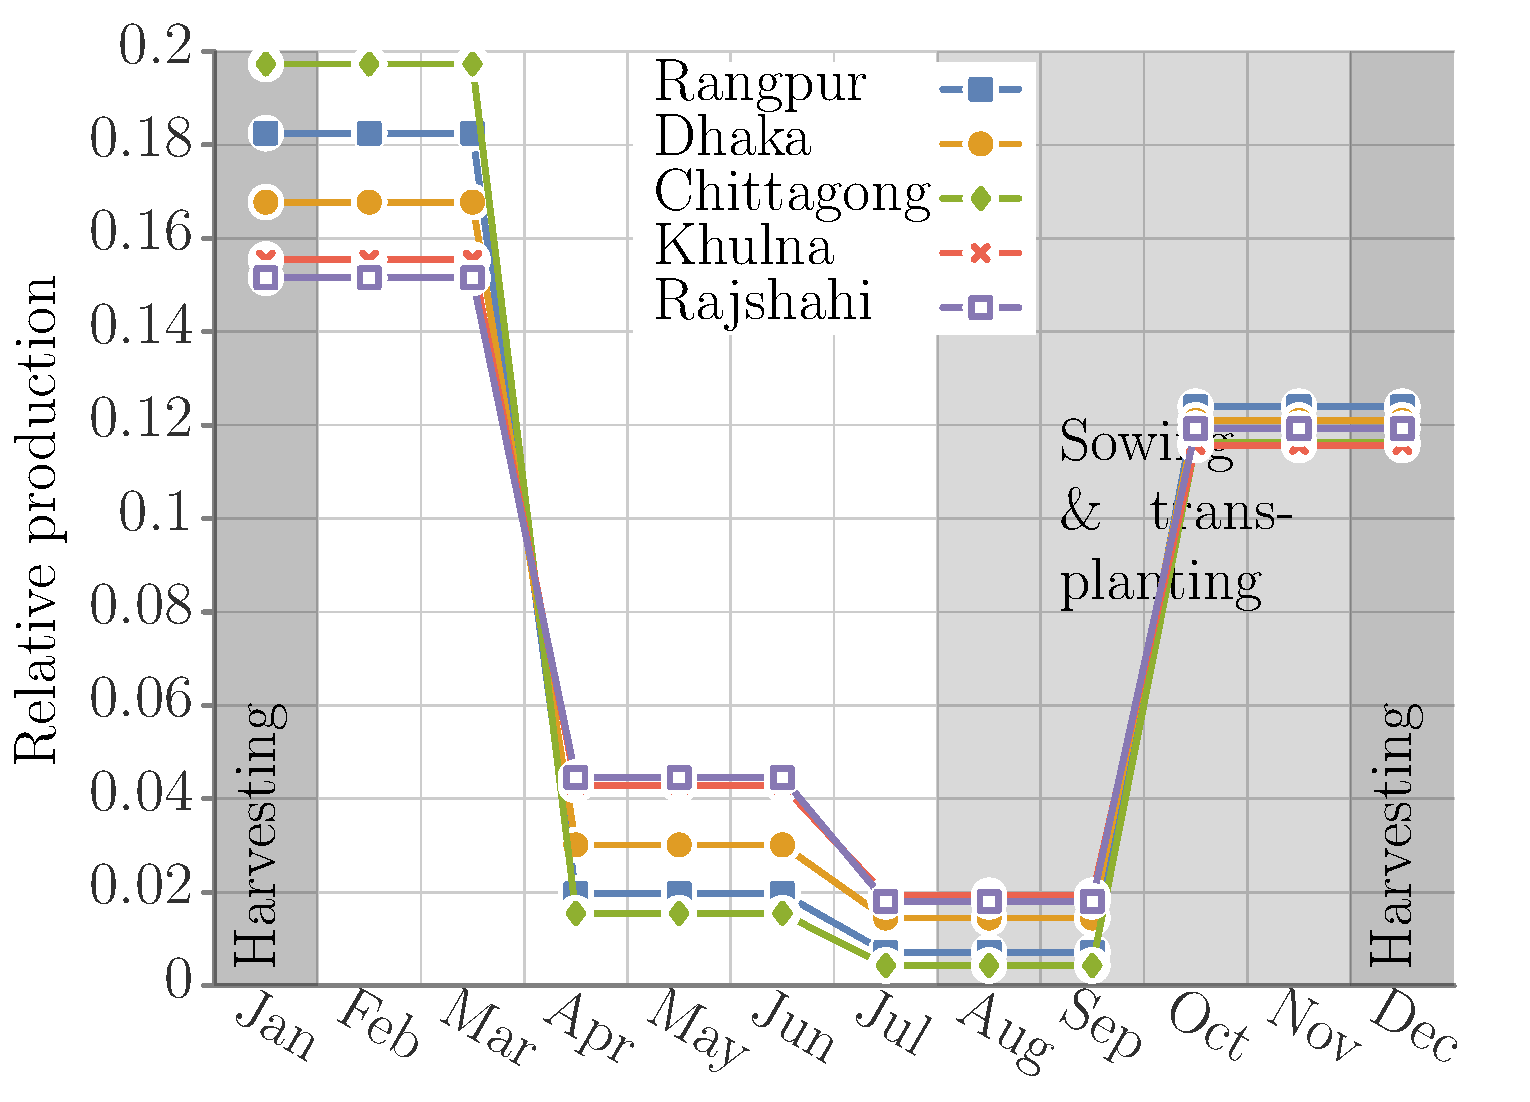
\includegraphics[width=\textwidth]{../production/results/prod_tomato_BGD.pdf}
\caption{Bangladesh tomato production compared with growing season
    information~\cite{bbs2017}}
\end{subfigure}
\begin{subfigure}[b]{.32\textwidth}
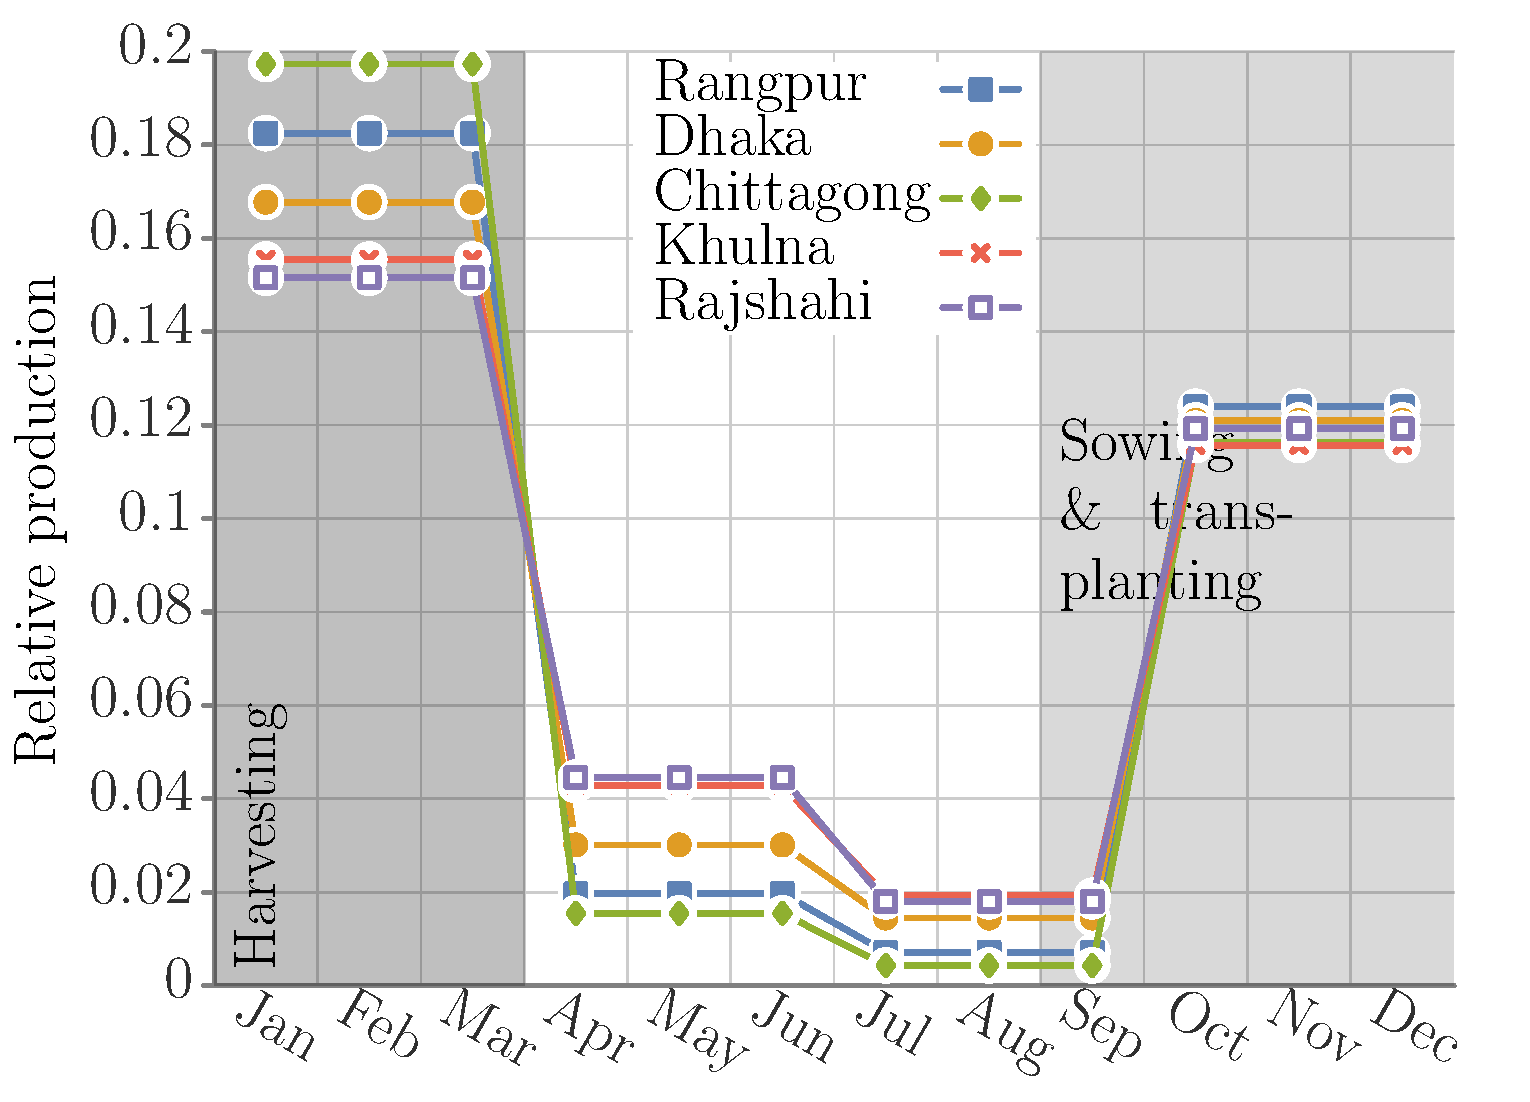
\includegraphics[width=\textwidth]{../production/results/prod_potato_BGD.pdf}
\caption{Bangladesh potato production compared with growing season
    information~\cite{bbs2017}}
\end{subfigure}
\begin{subfigure}[b]{.32\textwidth}
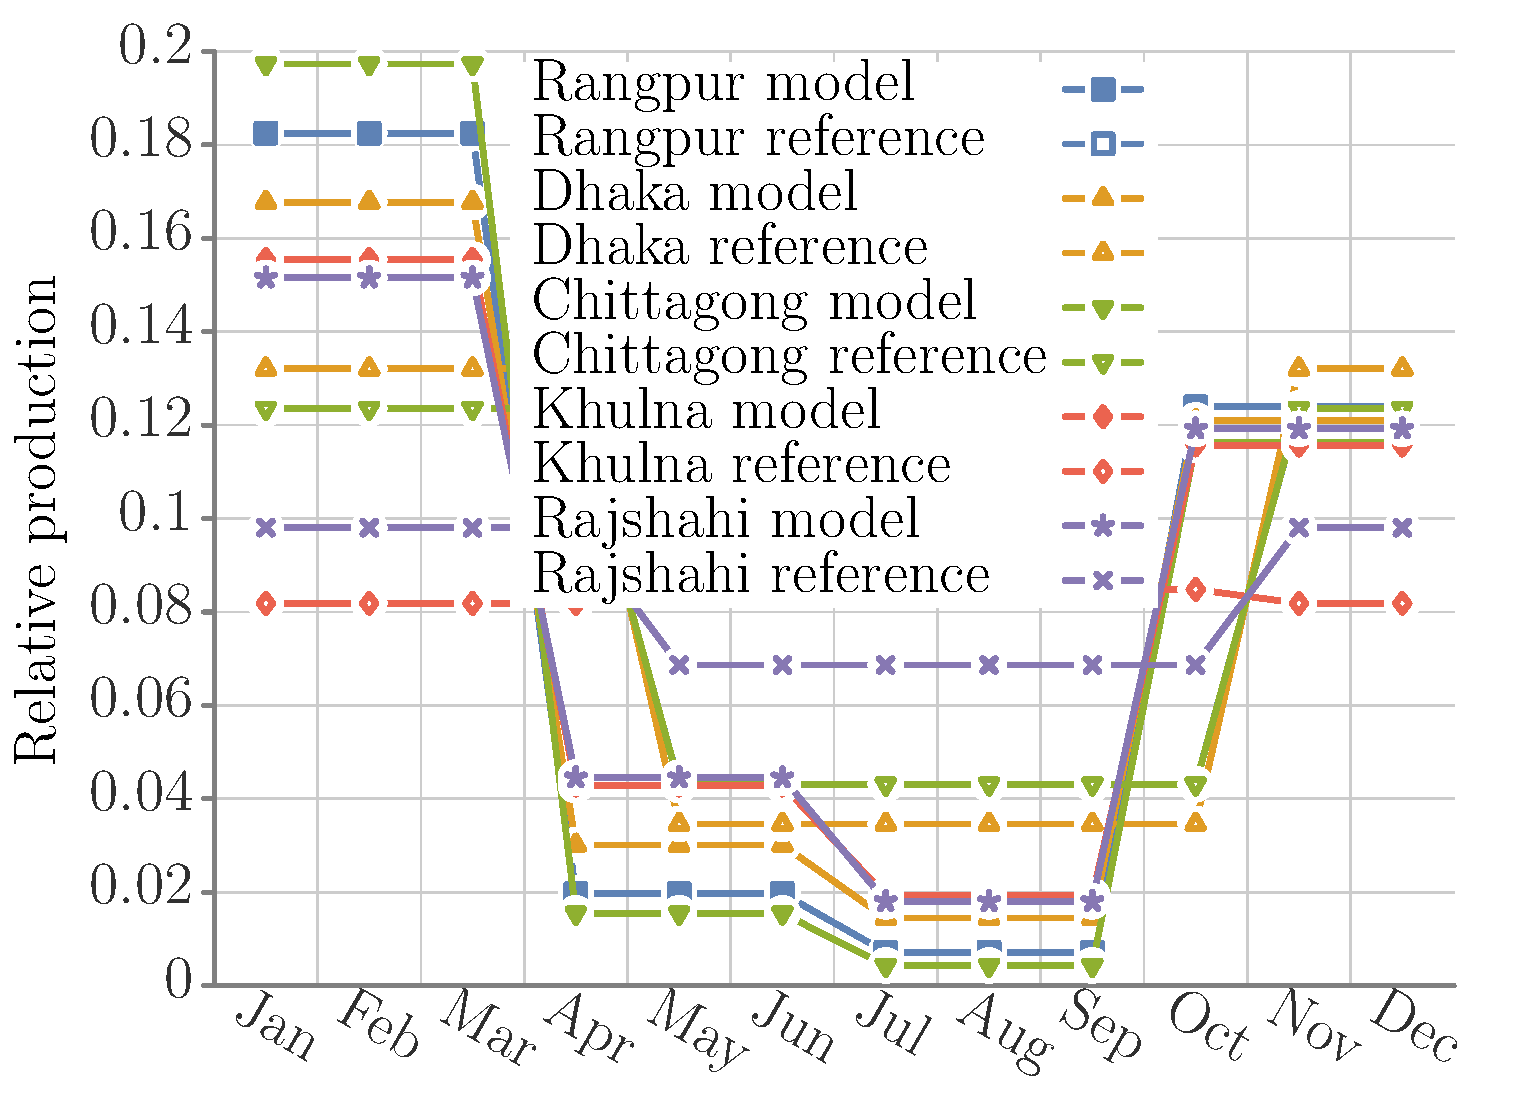
\includegraphics[width=\textwidth]{../production/results/prod_eggplant_BGD.pdf}
\caption{Bangladesh eggplant production compared with growing season
    information~\cite{bbs2017}}
\end{subfigure}
\begin{subfigure}[b]{.32\textwidth}
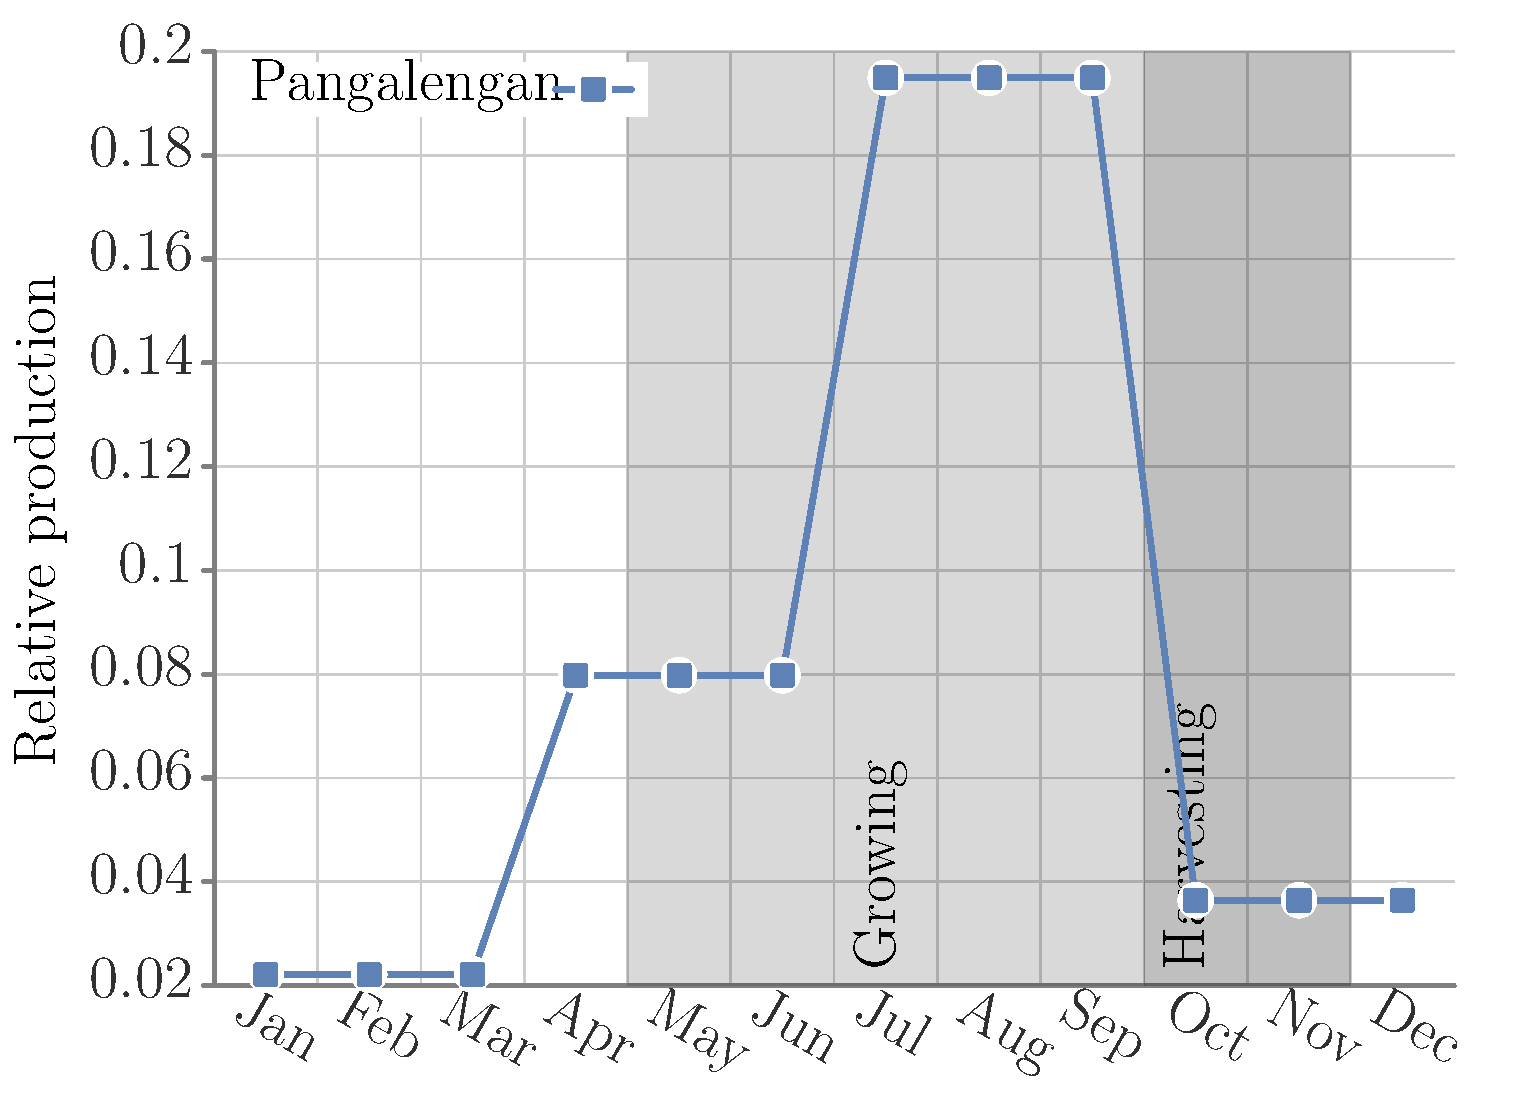
\includegraphics[width=\textwidth]{../production/results/prod_tomato_IDN.pdf}
\caption{Indonesia tomato production compared with growing season
    information~\cite{arsanti2015}}
\end{subfigure}
\begin{subfigure}[b]{.32\textwidth}
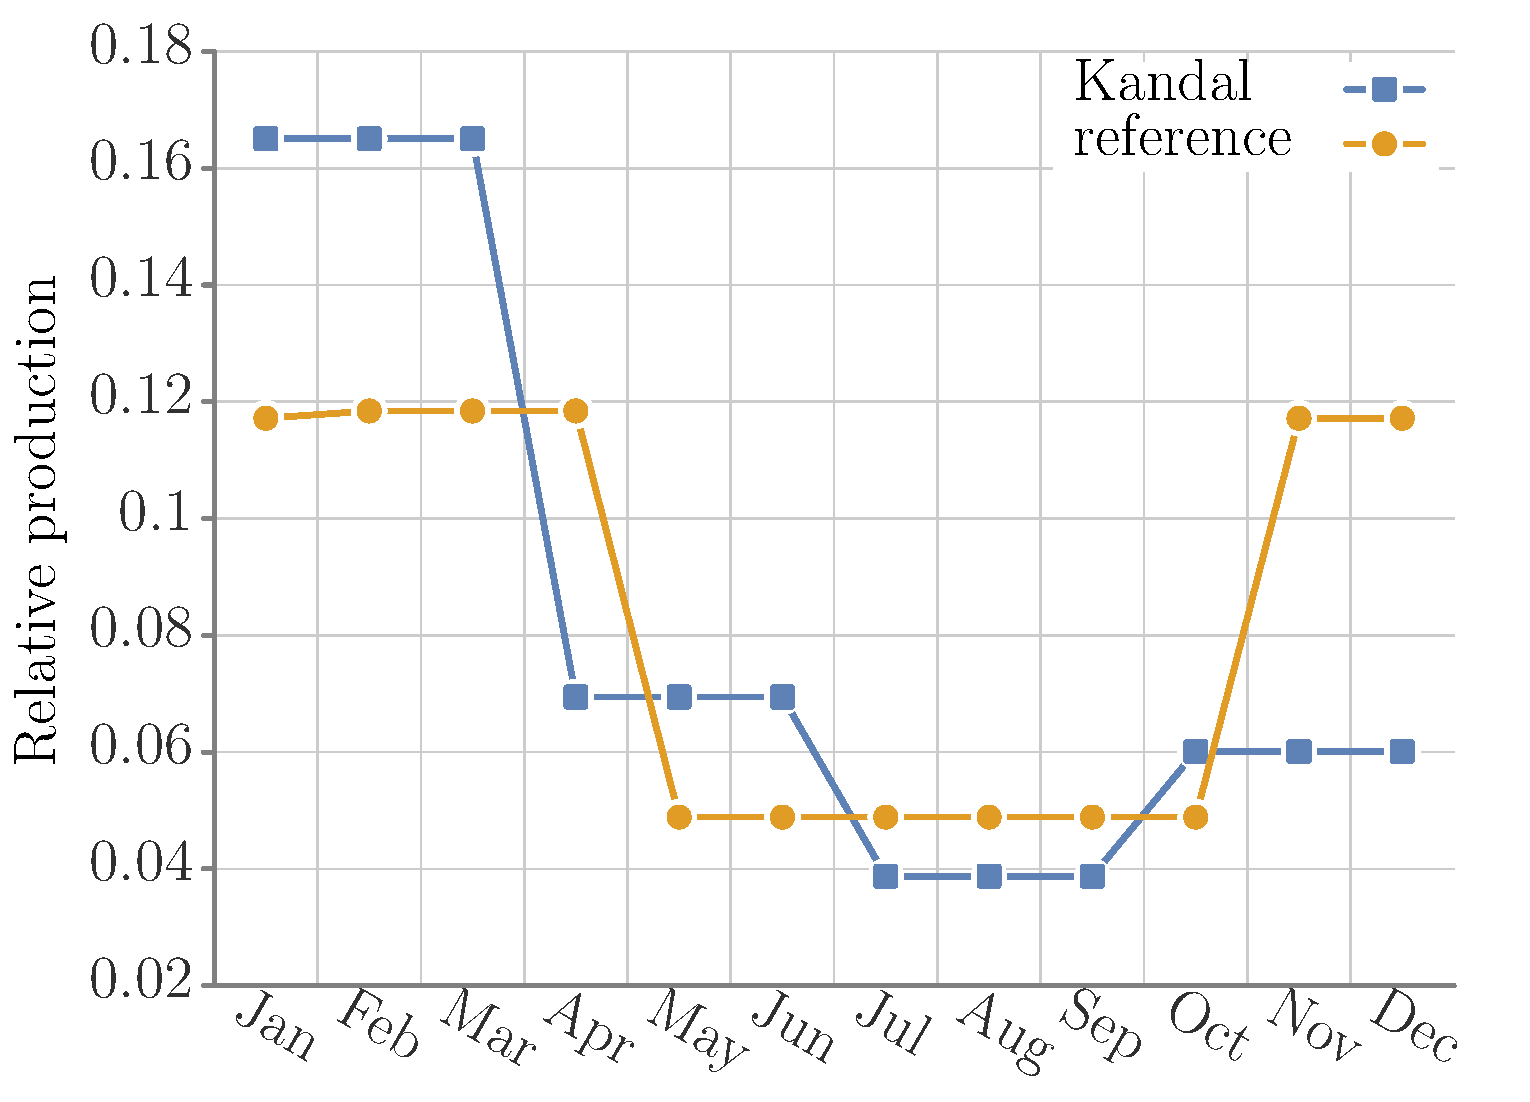
\includegraphics[width=\textwidth]{../production/results/prod_tomato_KHM.pdf}
\caption{Cambodia tomato production compared with seasonal production
    information~\cite{genova2006postharvest}}
\end{subfigure}
\begin{subfigure}[b]{.32\textwidth}
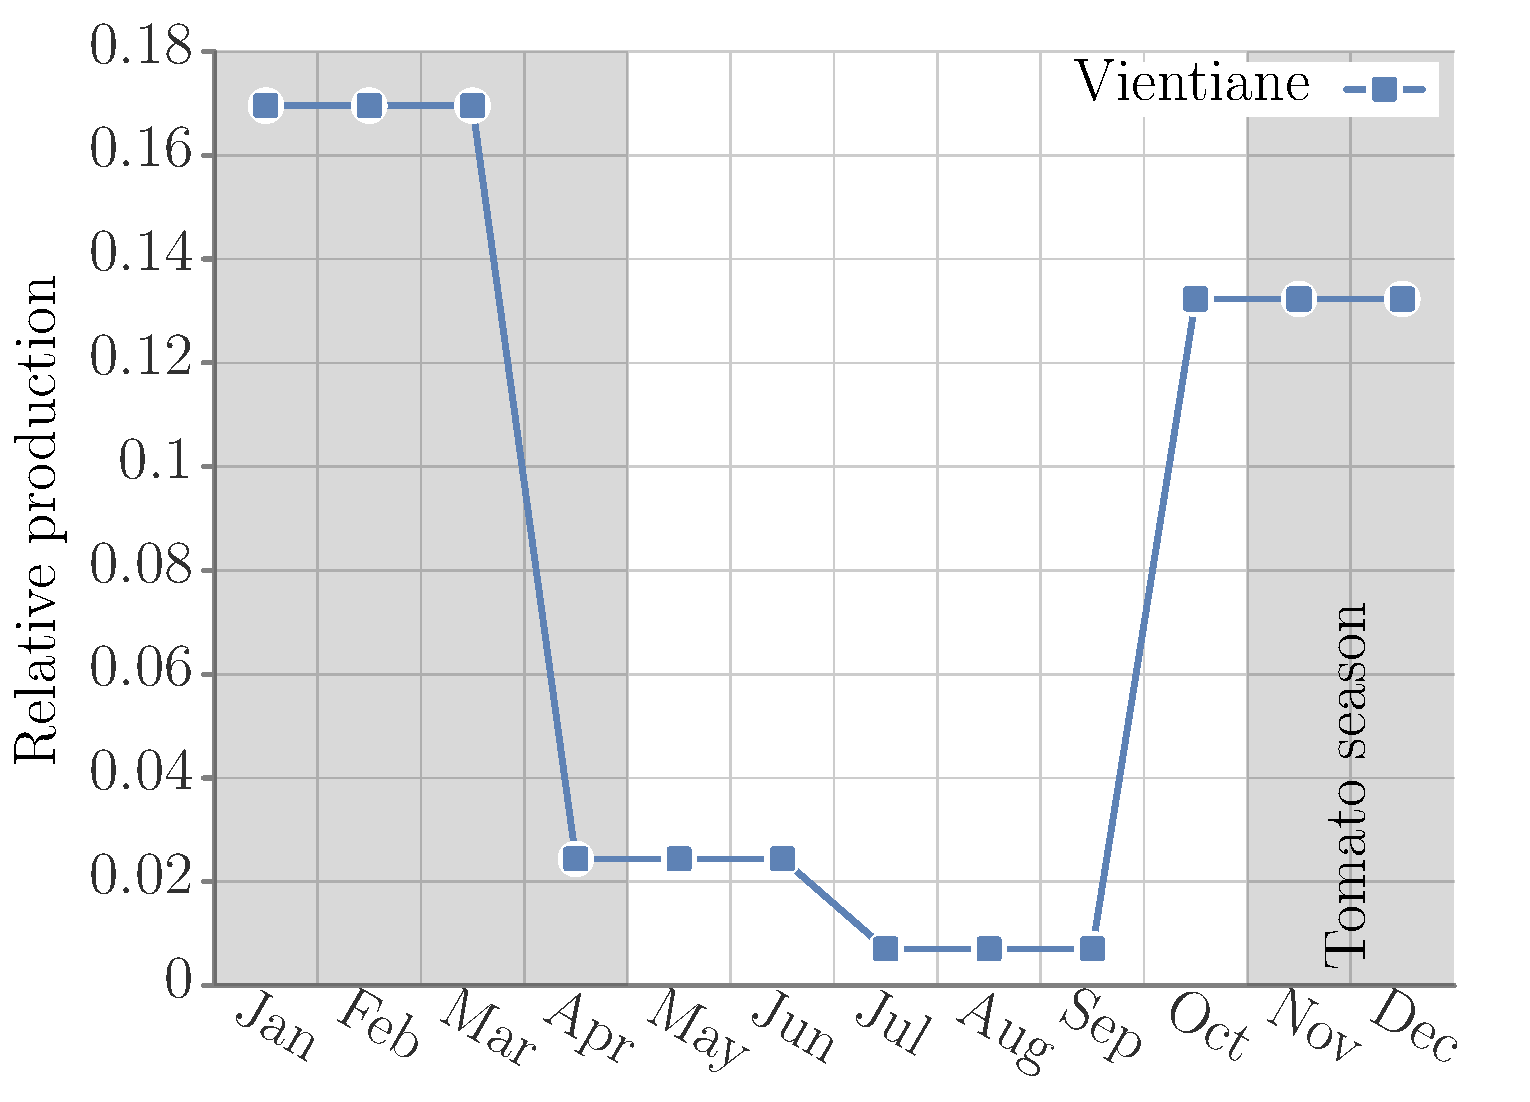
\includegraphics[width=\textwidth]{../production/results/prod_tomato_LAO.pdf}
\caption{Laos tomato production compared with growing season
    information~\cite{kethonga2004}}
\end{subfigure}
\begin{subfigure}[b]{.32\textwidth}
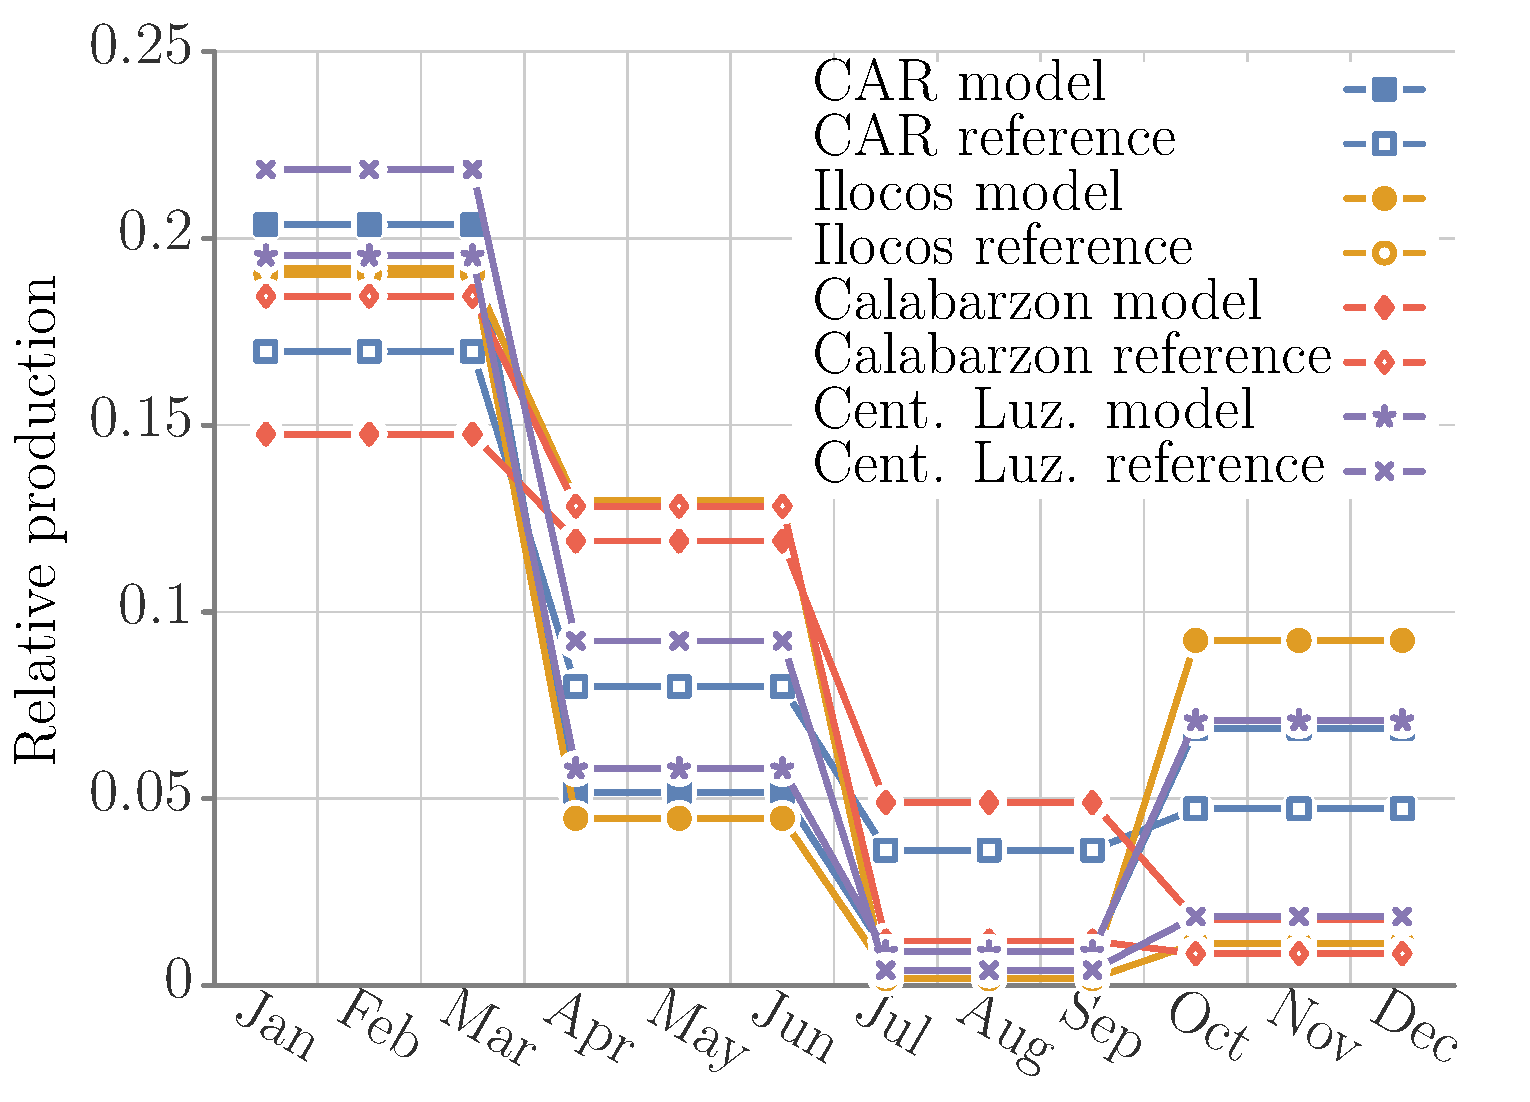
\includegraphics[width=\textwidth]{../production/results/prod_tomato_PHL_north.pdf}
\caption{Philippines tomato production compared with growing season
    information~\cite{psa2017} (North)}
\end{subfigure}
\begin{subfigure}[b]{.32\textwidth}
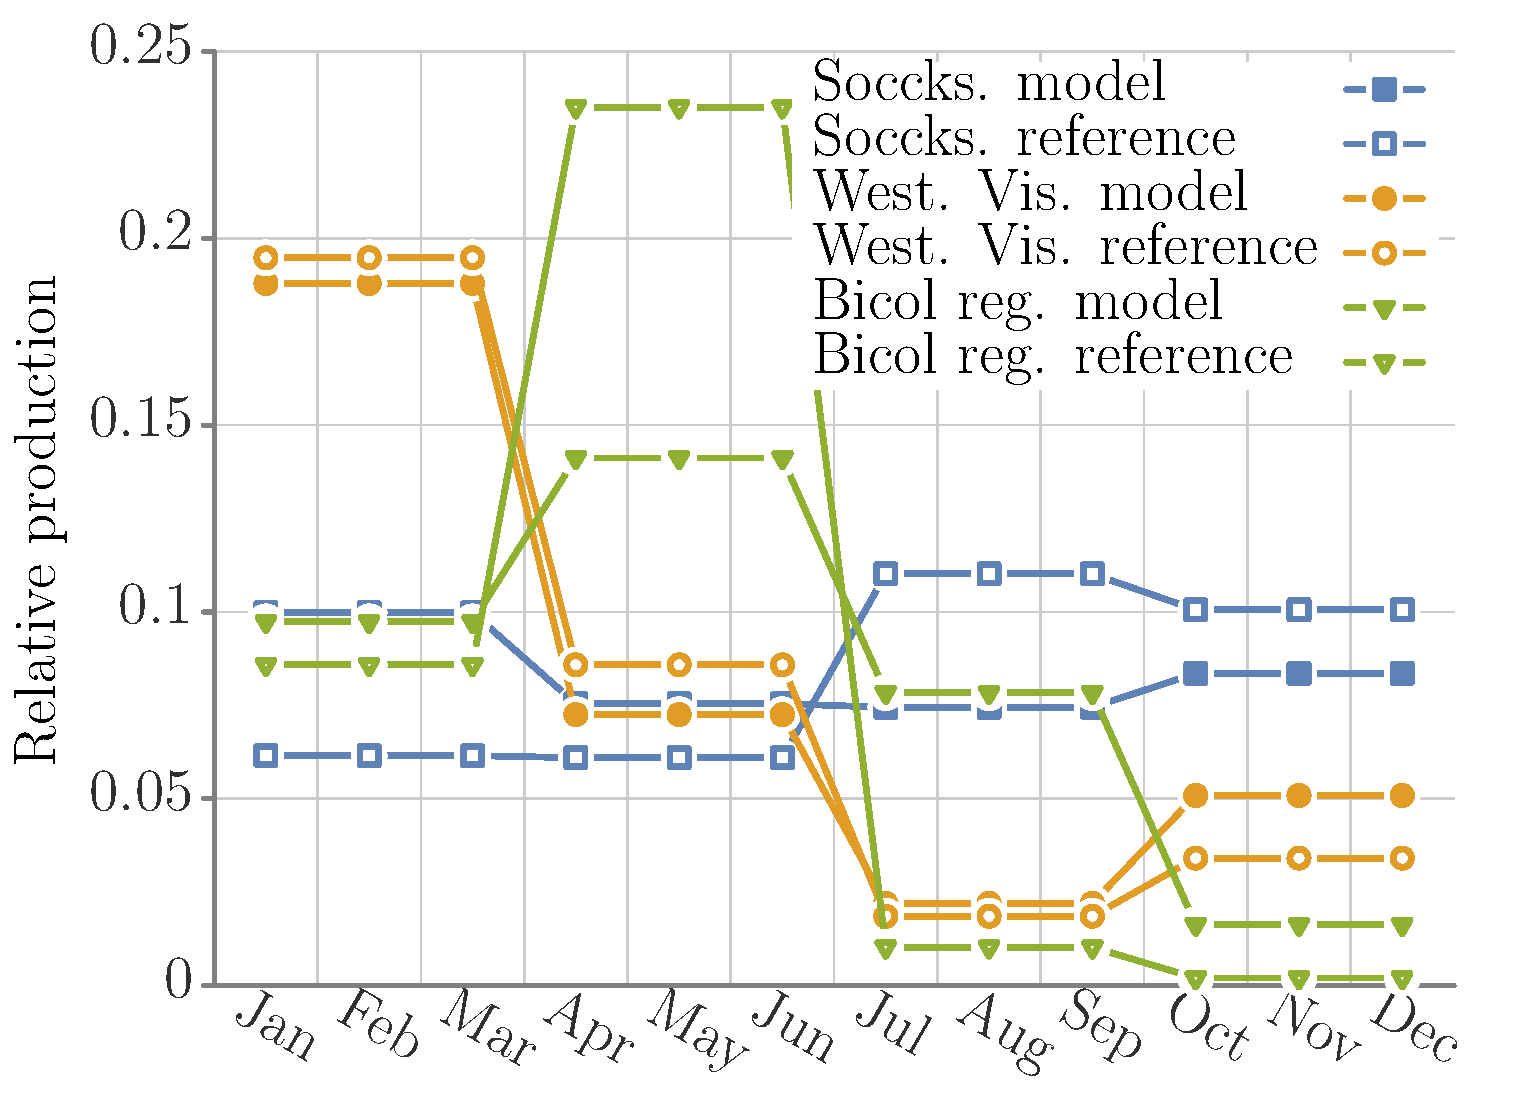
\includegraphics[width=\textwidth]{../production/results/prod_tomato_PHL_central.pdf}
\caption{Philippines tomato production compared with growing season
    information~\cite{psa2017} (Central and South)}
\end{subfigure}
\begin{subfigure}[b]{.32\textwidth}
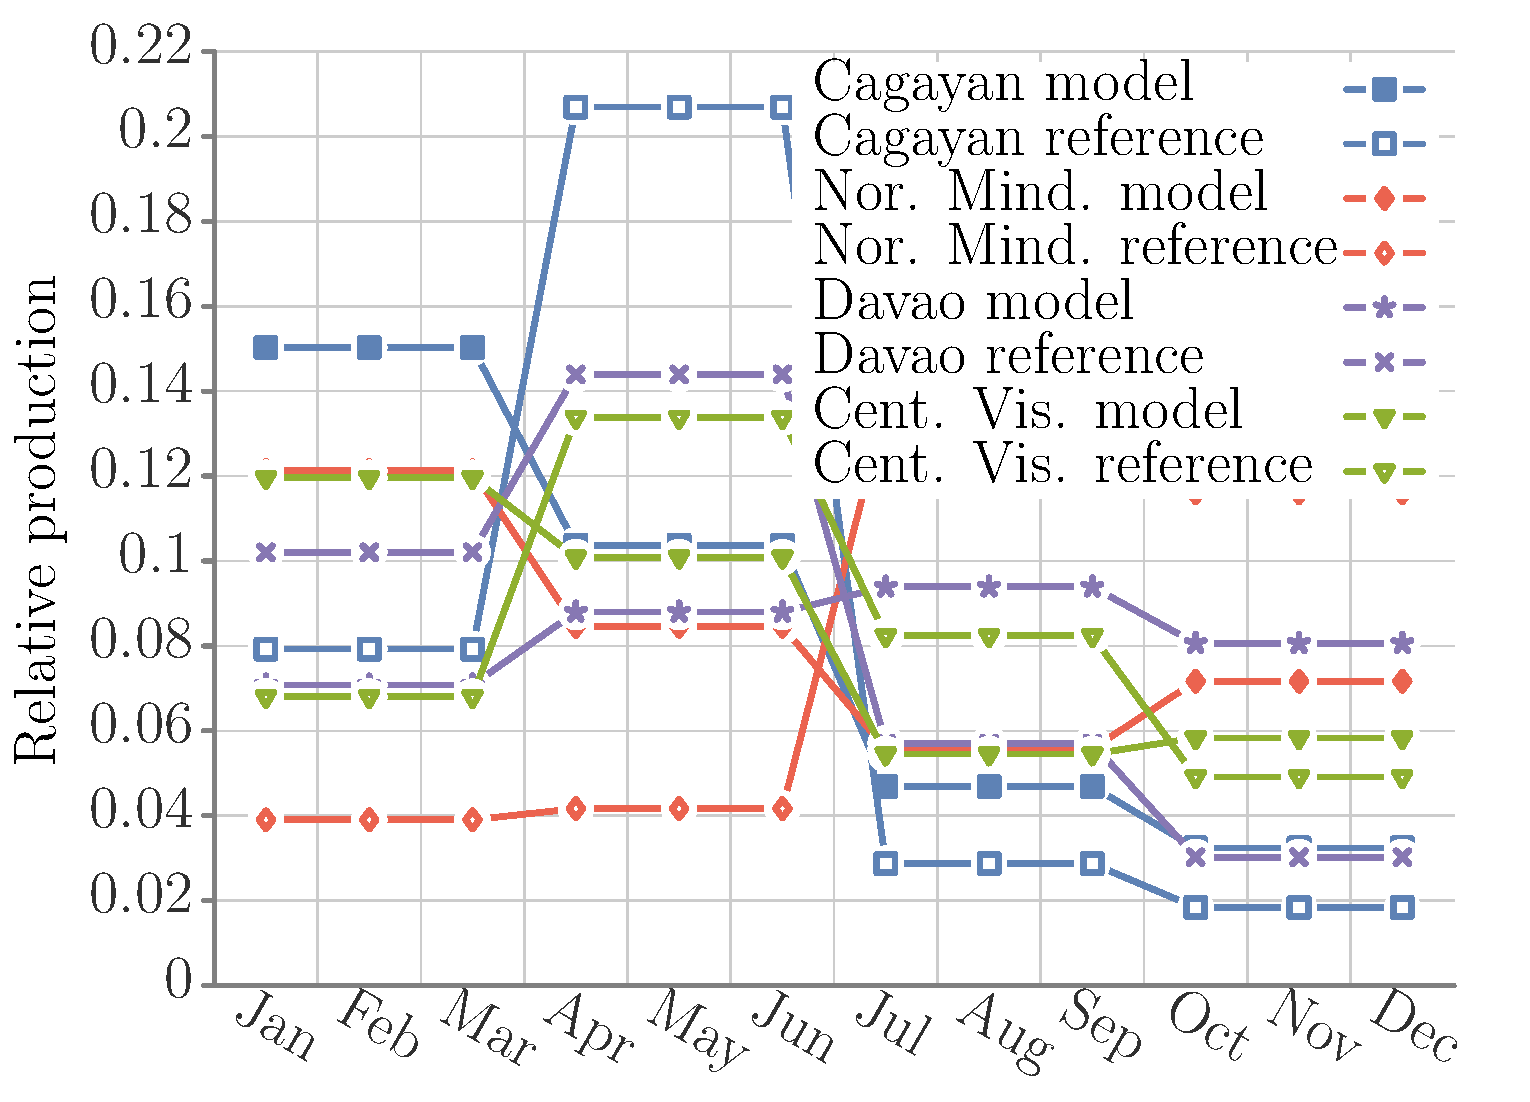
\includegraphics[width=\textwidth]{../production/results/prod_tomato_PHL_exceptions.pdf}
\caption{Philippines tomato production compared with growing season
    information~\cite{psa2017}: Regions with mismatch.}
\end{subfigure}
\caption{Comparing relative production as per the regression model with
quantitative/qualitative reports for different regions.
\label{fig:seasonalProd}}
\end{figure}
%%
%% \begin{figure}
%% \label{fig:sa}
%% \vspace{-5cm}
%% 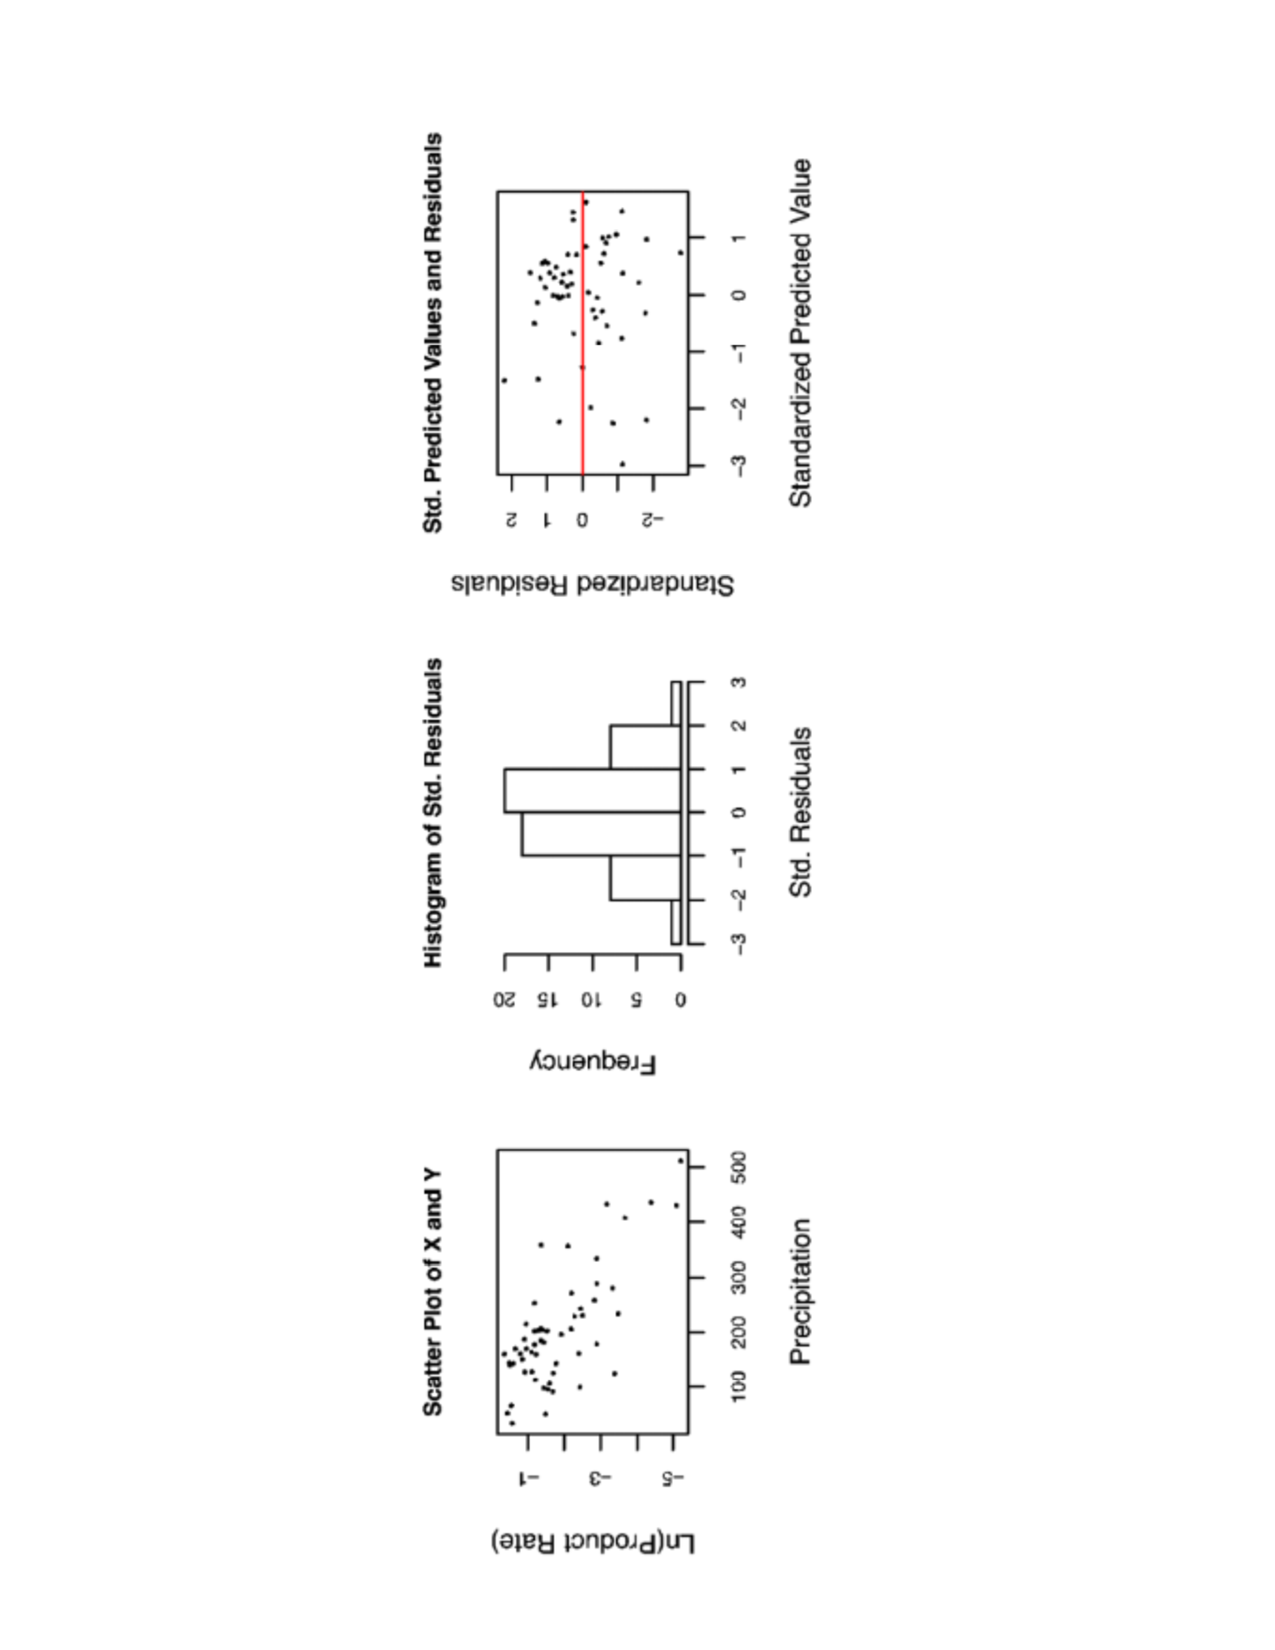
\includegraphics[width=0.8\textwidth,angle=-90,origin=c]{figs/SA_image.pdf}
%% \vspace{-7cm}
%% \caption{Validation of Linearity, Normality, and Homogeneity}
%
%\end{figure}
\subsection{Production, consumption, imports, exports and processing}
\label{sec:locAttrib}
%% For consumption, we used
%% country-level production~\cite{consumption}, which was available for half
%% of the countries. For Singapore, we estimated it as the difference between
%% total inflow (production and imports) and total outflow (exports) based on
%% FAO data. For Vietnam, Wijk~et~al.~\cite{wijk2007} provides this
%% information. For Myanmar, Cambodia and Laos, we found no information. We
%% used median consumption for the region. We also analyzed consumption with
%% respect to per capita gross domestic product (GDP). However, we did not
%% find any correlation between GDP and consumption both globally as well as
%% restricted to the study region. 

Monthly tomato production (consumption) at a locality was obtained by aggregating
production (population) at all cells that belong to it. Population data was
obtained from Landscan (Table~\ref{tab:data}).
For most countries, imports and exports are a small fraction of domestic
production. The main
exceptions were the significant tomato imports from India to Bangladesh and
trade between Malaysia and Singapore. We identified major routes of trade
from India to Bangladesh~\cite{EIIndia2015} and the total imports from
India (FAOSTAT) was distributed uniformly between three cities close to the
border with India along these routes. Finally, these imports were evenly
distributed for the later half of the year since Bangladesh imports mostly
during the rainy season. To capture the significant trade between Singapore
and Malaysia, we included Singapore in the domestic flow network of
Malaysia as there is high interaction between the two countries.  The
resulting flow from the gravity model from Malaysia to Singapore was
obtained by aggregating network flows across months and across edges with
Singapore as destination. This flow was comparable to the annual imports
from Malaysia to Singapore. With the exception for
Thailand~\cite{mict2013}, Vietnam~\cite{wijk2007} and Cambodia (pers.
comm.), there is no information on the amount of tomato production consumed
by the processing industry even though there is evidence of processing
industry in Malaysia and Indonesia. For each locality in Thailand, we
scaled the monthly production by the ratio annual production of fresh
tomatoes over total annual production (fresh and processed).

%UNCOMMENT
\subsection{Validation of domestic trade flows}
\label{sec:tradeFlows}
Since no market-to-market flow data is available for the region, we
searched the literature for evidence of tomato trade between cities or
regions for each country. Even this information is hardly
available. The next step was to further generalize the search by
considering the flow of vegetables. The results of our comparison of the
networks obtained using gravity flow model with literature are shown
Figure~\ref{fig:trade_flows}. Our general observations
as follows: (i)~To obtain good representation of trade flow, at minimum,
region/state level data of production is required; and (ii)~densely populated
urban pockets are a good representation of consumption centers. Some country
specific details follow.
%%
\begin{figure}[!ht]
\centering
\subcaptionbox{Bangladesh\label{fig:bgdFlow}}
{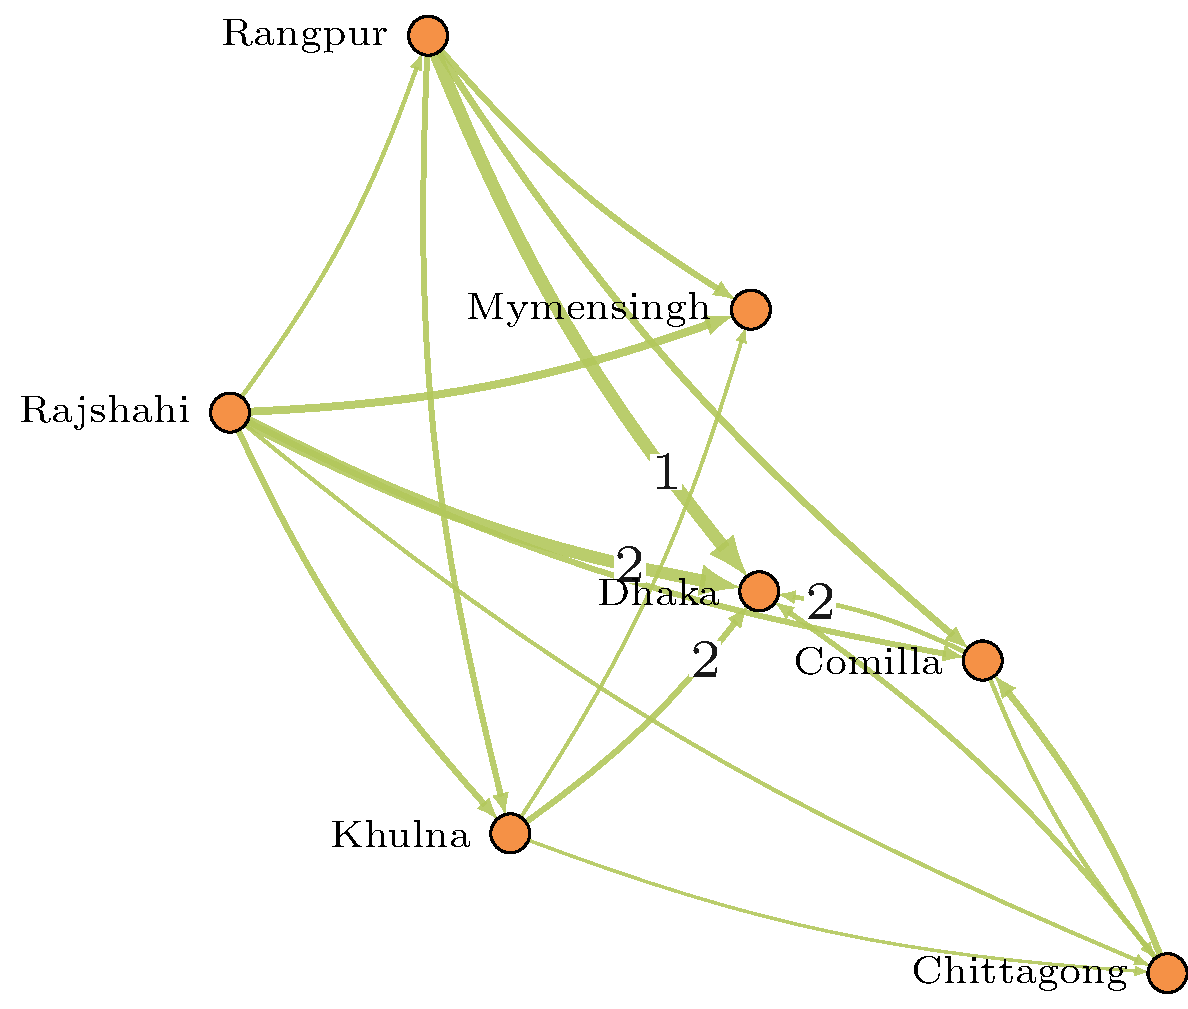
\includegraphics[width=.33\textwidth]{../long_distance/results/validation/BGD_flows_precip1_b2_k500.pdf}}
%%
\subcaptionbox{Myanmar\label{fig:mmrFlow}}
{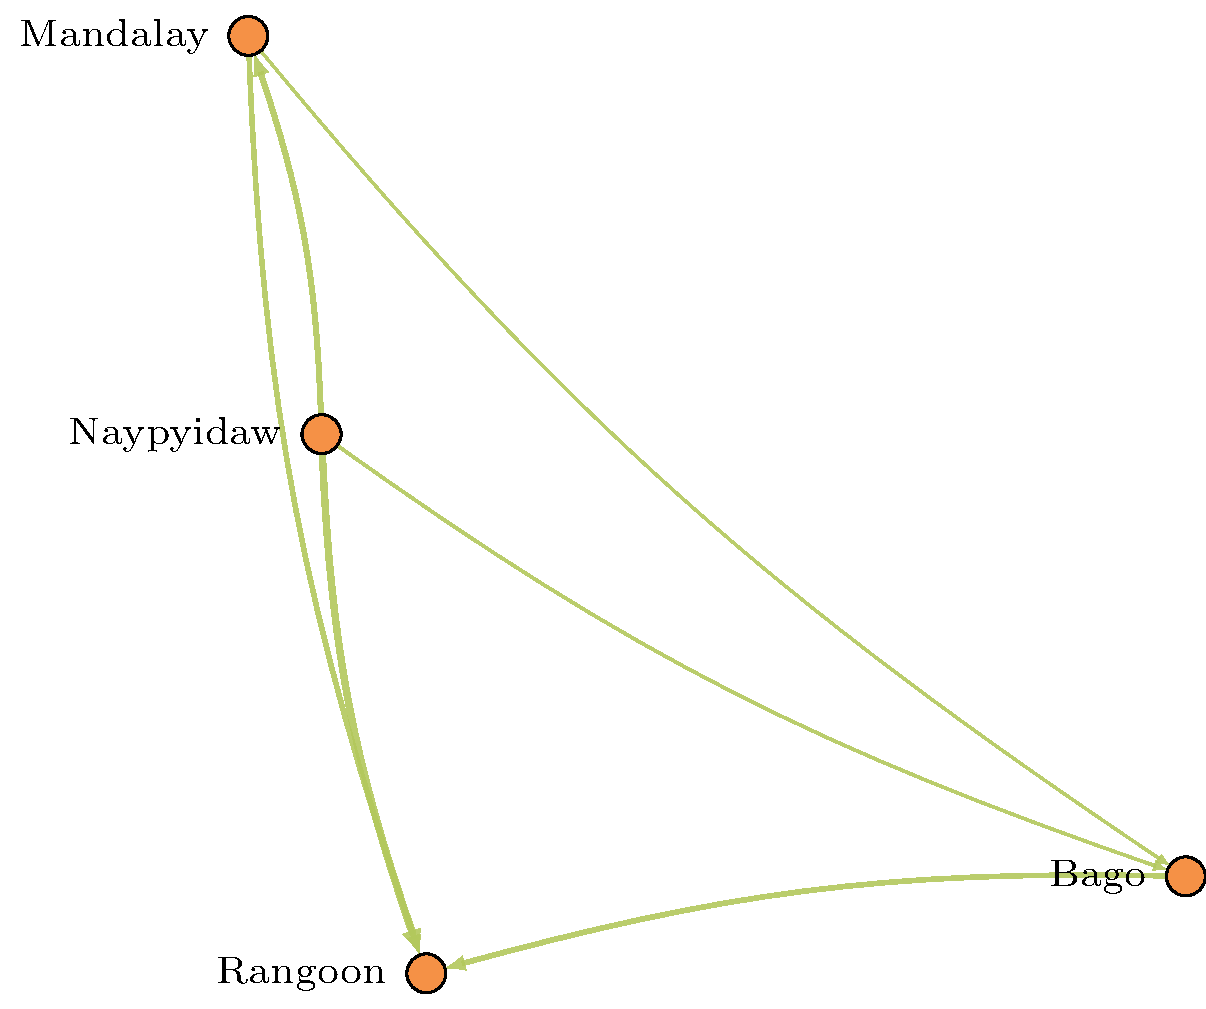
\includegraphics[width=.33\textwidth]{../long_distance/results/validation/MMR_flows_precip1_b2_k500.pdf}}
%%
\subcaptionbox{Thailand\label{fig:thaFlow}}
{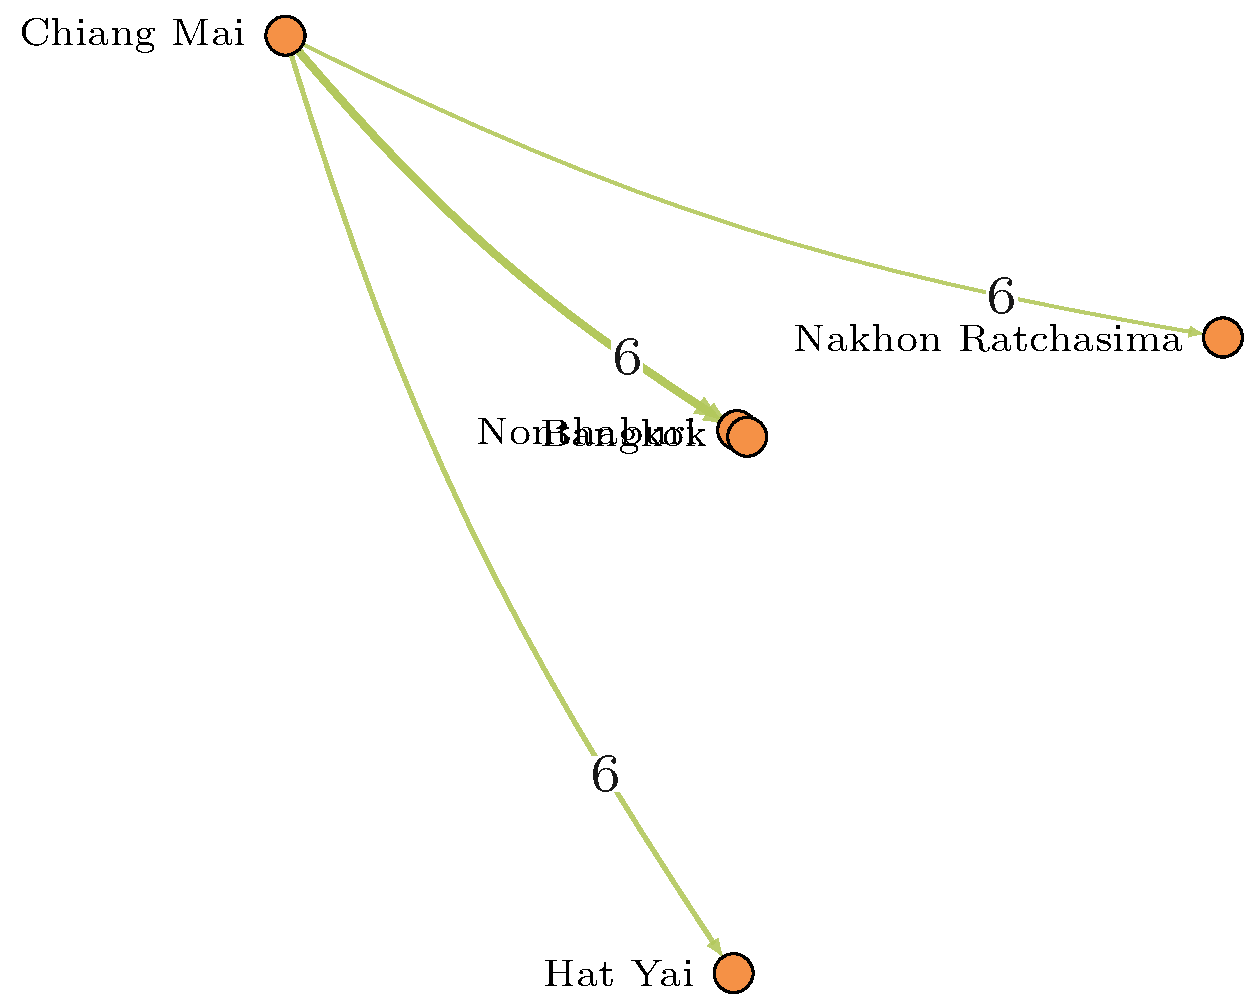
\includegraphics[width=.33\textwidth]{../long_distance/results/validation/THA_flows_precip1_b2_k500.pdf}}
%%
\subcaptionbox{Vietnam\label{fig:vnmFlow}}
{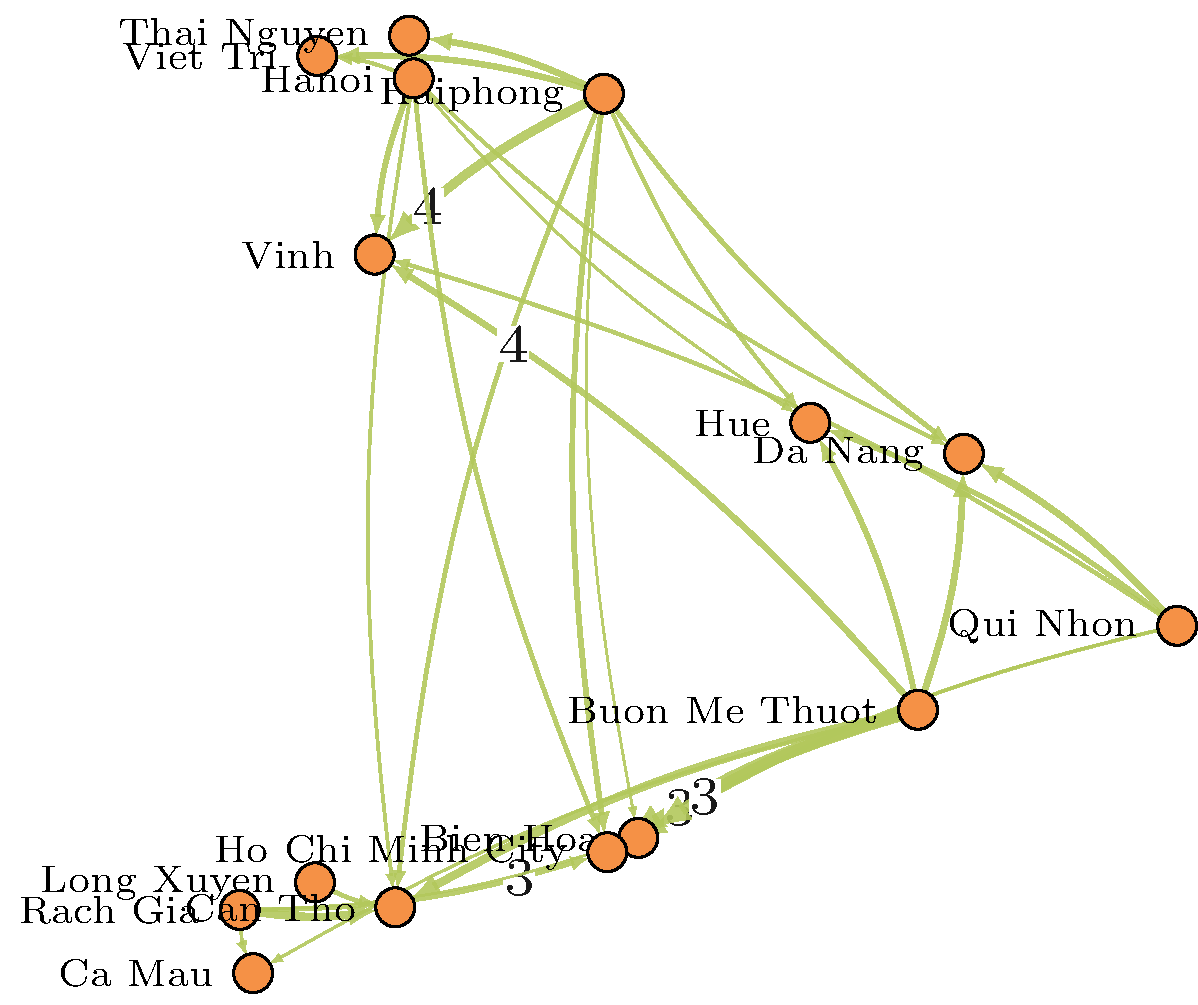
\includegraphics[width=.33\textwidth]{../long_distance/results/validation/VNM_flows_precip1_b2_k500.pdf}}
%%
\subcaptionbox{Malaysia and Singapore\label{fig:mysFlow}}
{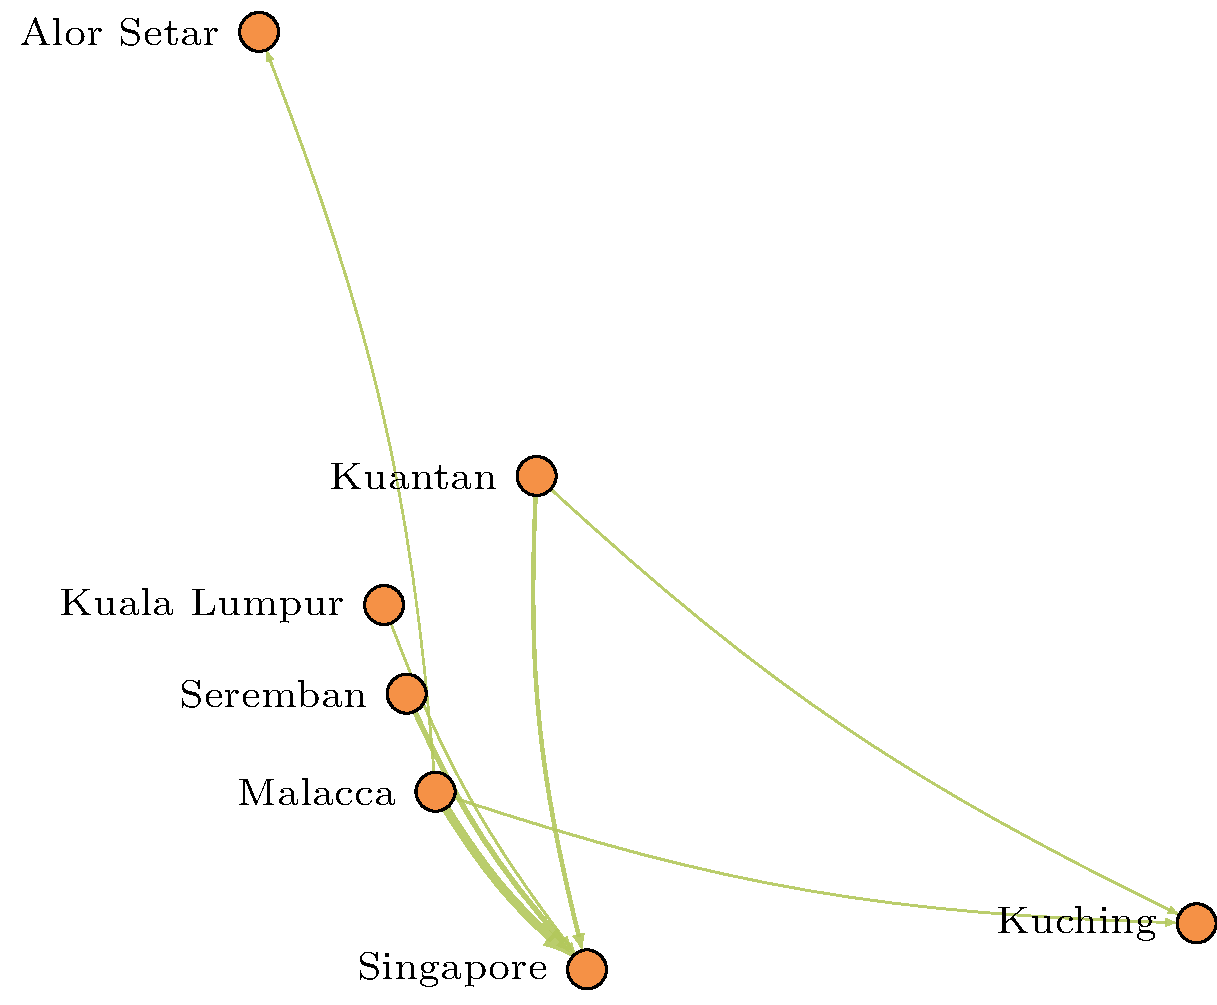
\includegraphics[width=.33\textwidth]{../long_distance/results/validation/MYS_flows_precip1_b2_k500.pdf}}
%%
\subcaptionbox{Indonesia\label{fig:idnFlow}}
{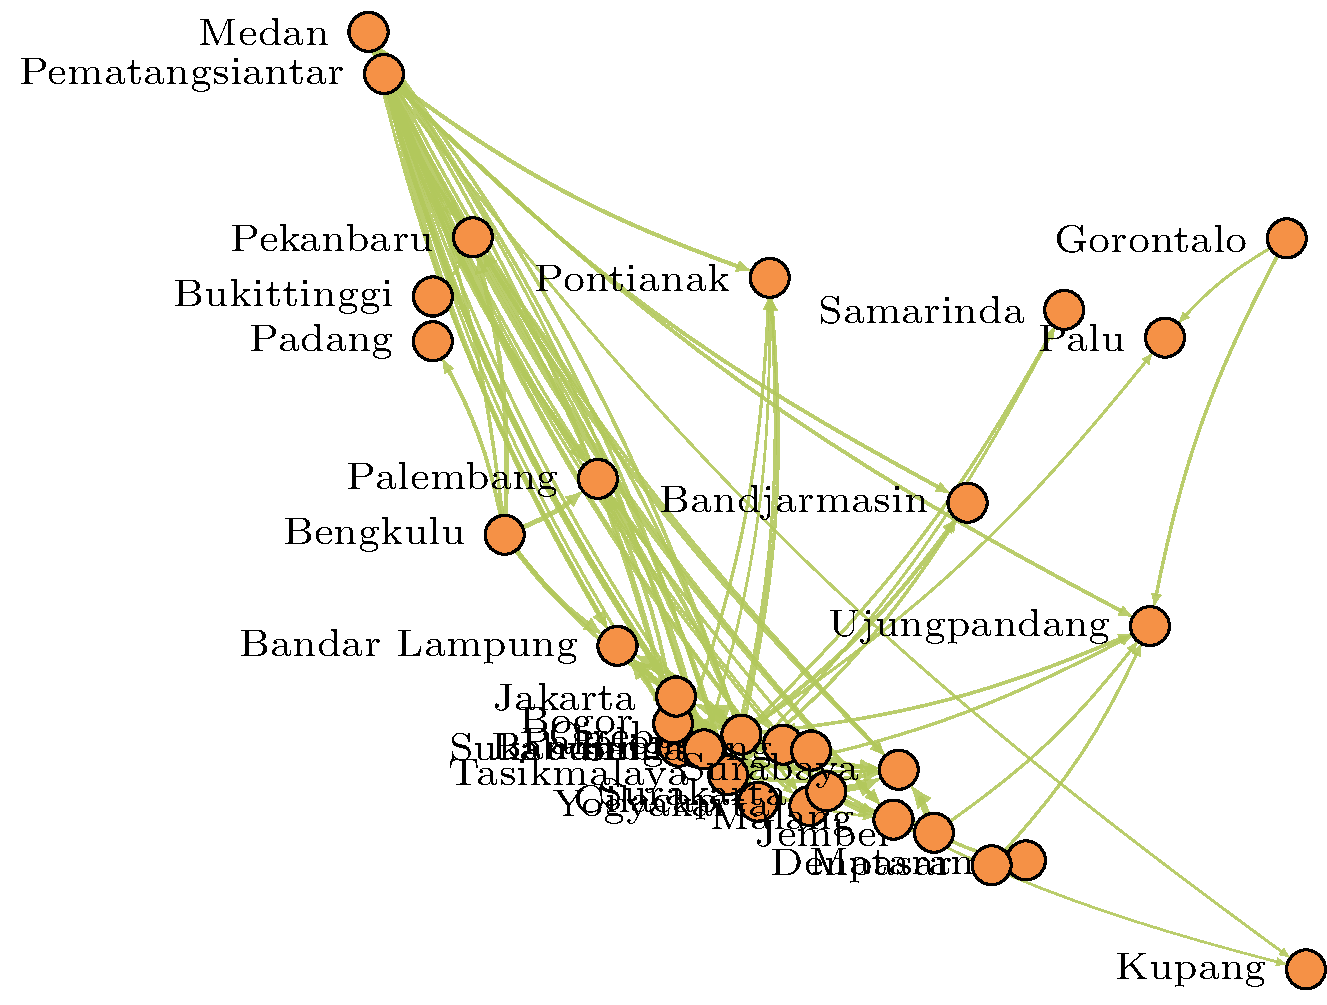
\includegraphics[width=.33\textwidth]{../long_distance/results/validation/IDN_flows_precip1_b2_k500.pdf}}
%%
\subcaptionbox{Philippines\label{fig:phlFlow}}
{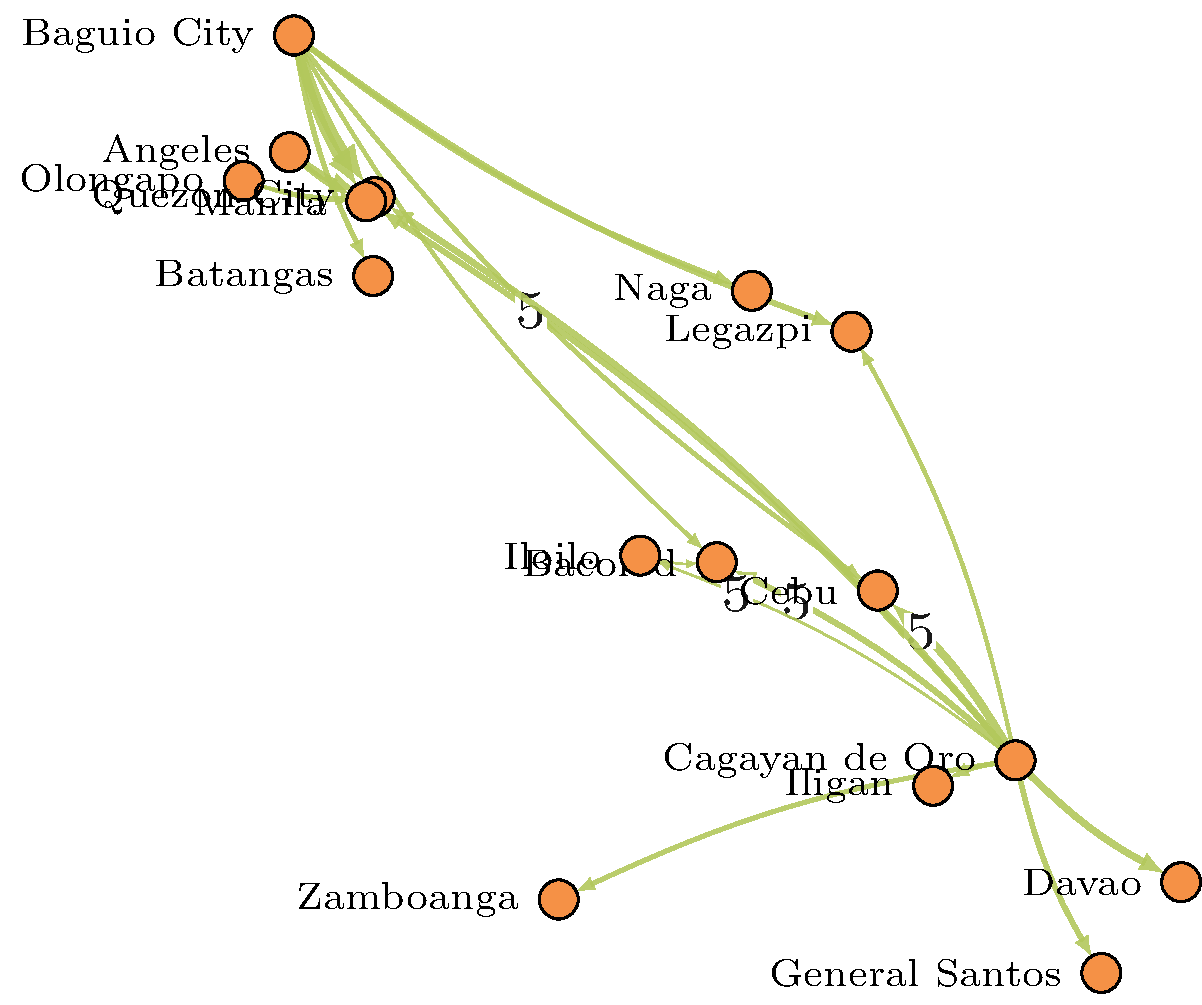
\includegraphics[width=.33\textwidth]{../long_distance/results/validation/PHL_flows_precip1_b2_k500.pdf}}
%%
\subcaptionbox{References corresponding to trade flow
evidence.}[.5\textwidth]{
    \small
\begin{tabular}{cl}
\hline
Index & Citation \\\hline
1 & Daily Sun 2018 \cite{dailysun2018}\\
2 & Karim et al. 2016 \cite{karim2016}\\
3 & Cadilhon et al. 2006 \cite{cadilhon2006}\\
4 & Wijk et al. 2007 \cite{wijk2007}\\
5 & Ledesma 2011 \cite{ledesma2011}\\
6 & Johnson et al. 2008 \cite{johnson2008}\\\hline
\end{tabular}
}
\caption{\textbf{Long-distance annual trade flows resulting from the gravity model.}
We combined monthly flows and to avoid clutter, we have displayed only major
    flows ($>500$). Some of the edges
    are labeled based on information from literature. The references
    corresponding to the labels are listed in (h). For Laos, Cambodia and
    Brunei, there are no flows as there is only one locality in each
    country. \label{fig:trade_flows}}
\end{figure}
%%
\paragraph{Bangladesh.}
There is evidence of vegetable flow from Rangpur region to Dhaka
particularly during winter~\cite{dailysun2018,independent2018}. The flow
from Southwest Bangladesh to Dhaka~\cite{karim2016} is captured by the edge
from Khulna to Dhaka (Figure~\ref{fig:bgdFlow}). We assigned import of
tomato from India to cities in the border based on information on important
trade routes~\cite{EIIndia2015}.  Since, there is no data on volume, we
distributed it evenly.
%%
\paragraph{Vietnam.}
There are primarily two consumption centers: Ho Chi Minh City in the south
supplied by Central Highlands and the Mekong River Delta, and
Hanoi-Haiphong urban centers in the north supplied by Red River Delta. For
Ho Chi Minh City, Lam Dong is the main district that supplies
vegetables~\cite{cadilhon2006}.  In our model (Figure~\ref{fig:vnmFlow}),
this flow is represented by Buon Me Thuot--a city in Central Highlands--to
Ho Chi Minh City. Buon Me Thuot is less than 100kms away from the Lam Dong
province thus covering the production in the area. In the north, much of
the production surplus is assigned to the Haiphong locality, and therefore,
it acts as a big source for almost all localities in the north. Our network
also has some long distance edges from north to south. This is mostly due
to the large population in the south. There is not much evidence of this
flow and it could be a result of not accounting for heterogeneity in
consumption.
%%
\paragraph{Malaysia and Singapore.} We combined the locality corresponding
to Singapore with Malaysia, so that the flow between these two countries is
treated as a domestic flow as there is free movement of people and goods
between these countries. The gravity model flows from Malaysia to Singapore
is between 50,000--60,000 tonnes compared to $\approx30,000$ tonnes
according to FAOSTAT. However, our network does not capture the flow from
Cameron Highlands, major tomato producer to cities of Malaysia. This
shortcoming is mainly due to unavailability of state/province level tomato
production information.
%%
\paragraph{Philippines.} The major production centers are in Cagayan de Oro
and regions north of Manila. These are captured by our network
(Figure~\ref{fig:phlFlow}).

\subsection{Transmission probability}\label{trans}
At any given time~$t$, for a cell~$v$ and its neighbor~$v'$ corresponding
to the considered pathway, let $\infest(v',t)$ be the strength of
infestation at~$v'$. Let,~$\alpha$ be the transmission rate corresponding
to the pathway. Then, the probability that the pest will be introduced
to~$v$ from~$v'$ is given by~$1-\exp\big(-\alpha\infest(v',t)\big)$. The
function form is similar to that in~\cite{newman2002spread,meyers2007}, but with
contact time between two nodes replaced with strength of infestation. Also,~$\alpha$ can be interpreted as the transmission probability
per unit infestation. Since in our case production in the cell is used as a
surrogate for~$\infest(v',t)$, it can be interpreted as the
probability of infection per unit production. \\

This form of the infection probability function has been seen before in
epidemiological models
\cite{diekmann2000mathematical,hethcote1989periodicity,hethcote1994thousand},
both continuous and discrete time models. Diekmann~et~al.
\cite{diekmann2000mathematical} 
consider a continuous time SI model, and define the probability that an
individual will not be infected with a function which relates to the form
above, taking the exponent as an integral of the "force of infection". 
%% In \cite{cantor2003sas}, we see more complexity, but we also see some
%% derivation of this function form from the "proportional hazards model".
%% They similarly consider a continuous time model and an exponential
%% probability function of remaining susceptible.
In \cite{hethcote1994thousand}, we see a discrete time version of this
function form, with the probability of still being exposed after $t$ time
steps as: $P(t) = e^{-\epsilon t}$, where $\epsilon$ relates to the
"transfer rate". This function form was derived when considering
traditional SIR models mathematically in \cite{hethcote1989periodicity}.
\section{Parameterization and simulation}
\label{sec:cart}
For each parameter setting, we evaluated the model output by comparing it
with historical invasion data from Bangladesh using the maximum likelihood
estimation method for comparison as defined in the main document (see
definition of likelihood in equation~(\ref{M:eqn:likelihood})). Simulations
were run with 100 repetitions. From the output we computed the empirical
probability that a cell is in state~$I$ at time~$t$, which in turn was used
to compute likelihood.  We applied Classification and Regression
Trees~(CART) to guide parameter space exploration. Initially, the parameter
space was coarsely sampled. The parameter values are listed in
Table~\ref{M:tab:param}. For each of these samples, simulations were run
and the likelihood computed. With the model parameters as independent
variables and likelihood as the dependent variable, we analyzed the results
using CART (see Figure~\ref{fig:cart}). We chose parameter subspaces with
high likelihood (5.5 or more) and rejected those with lower values.  For
each chosen parameter subspace, the process was repeated.
%%
\begin{figure}[!ht]
    \begin{subfigure}[b]{.45\textwidth}
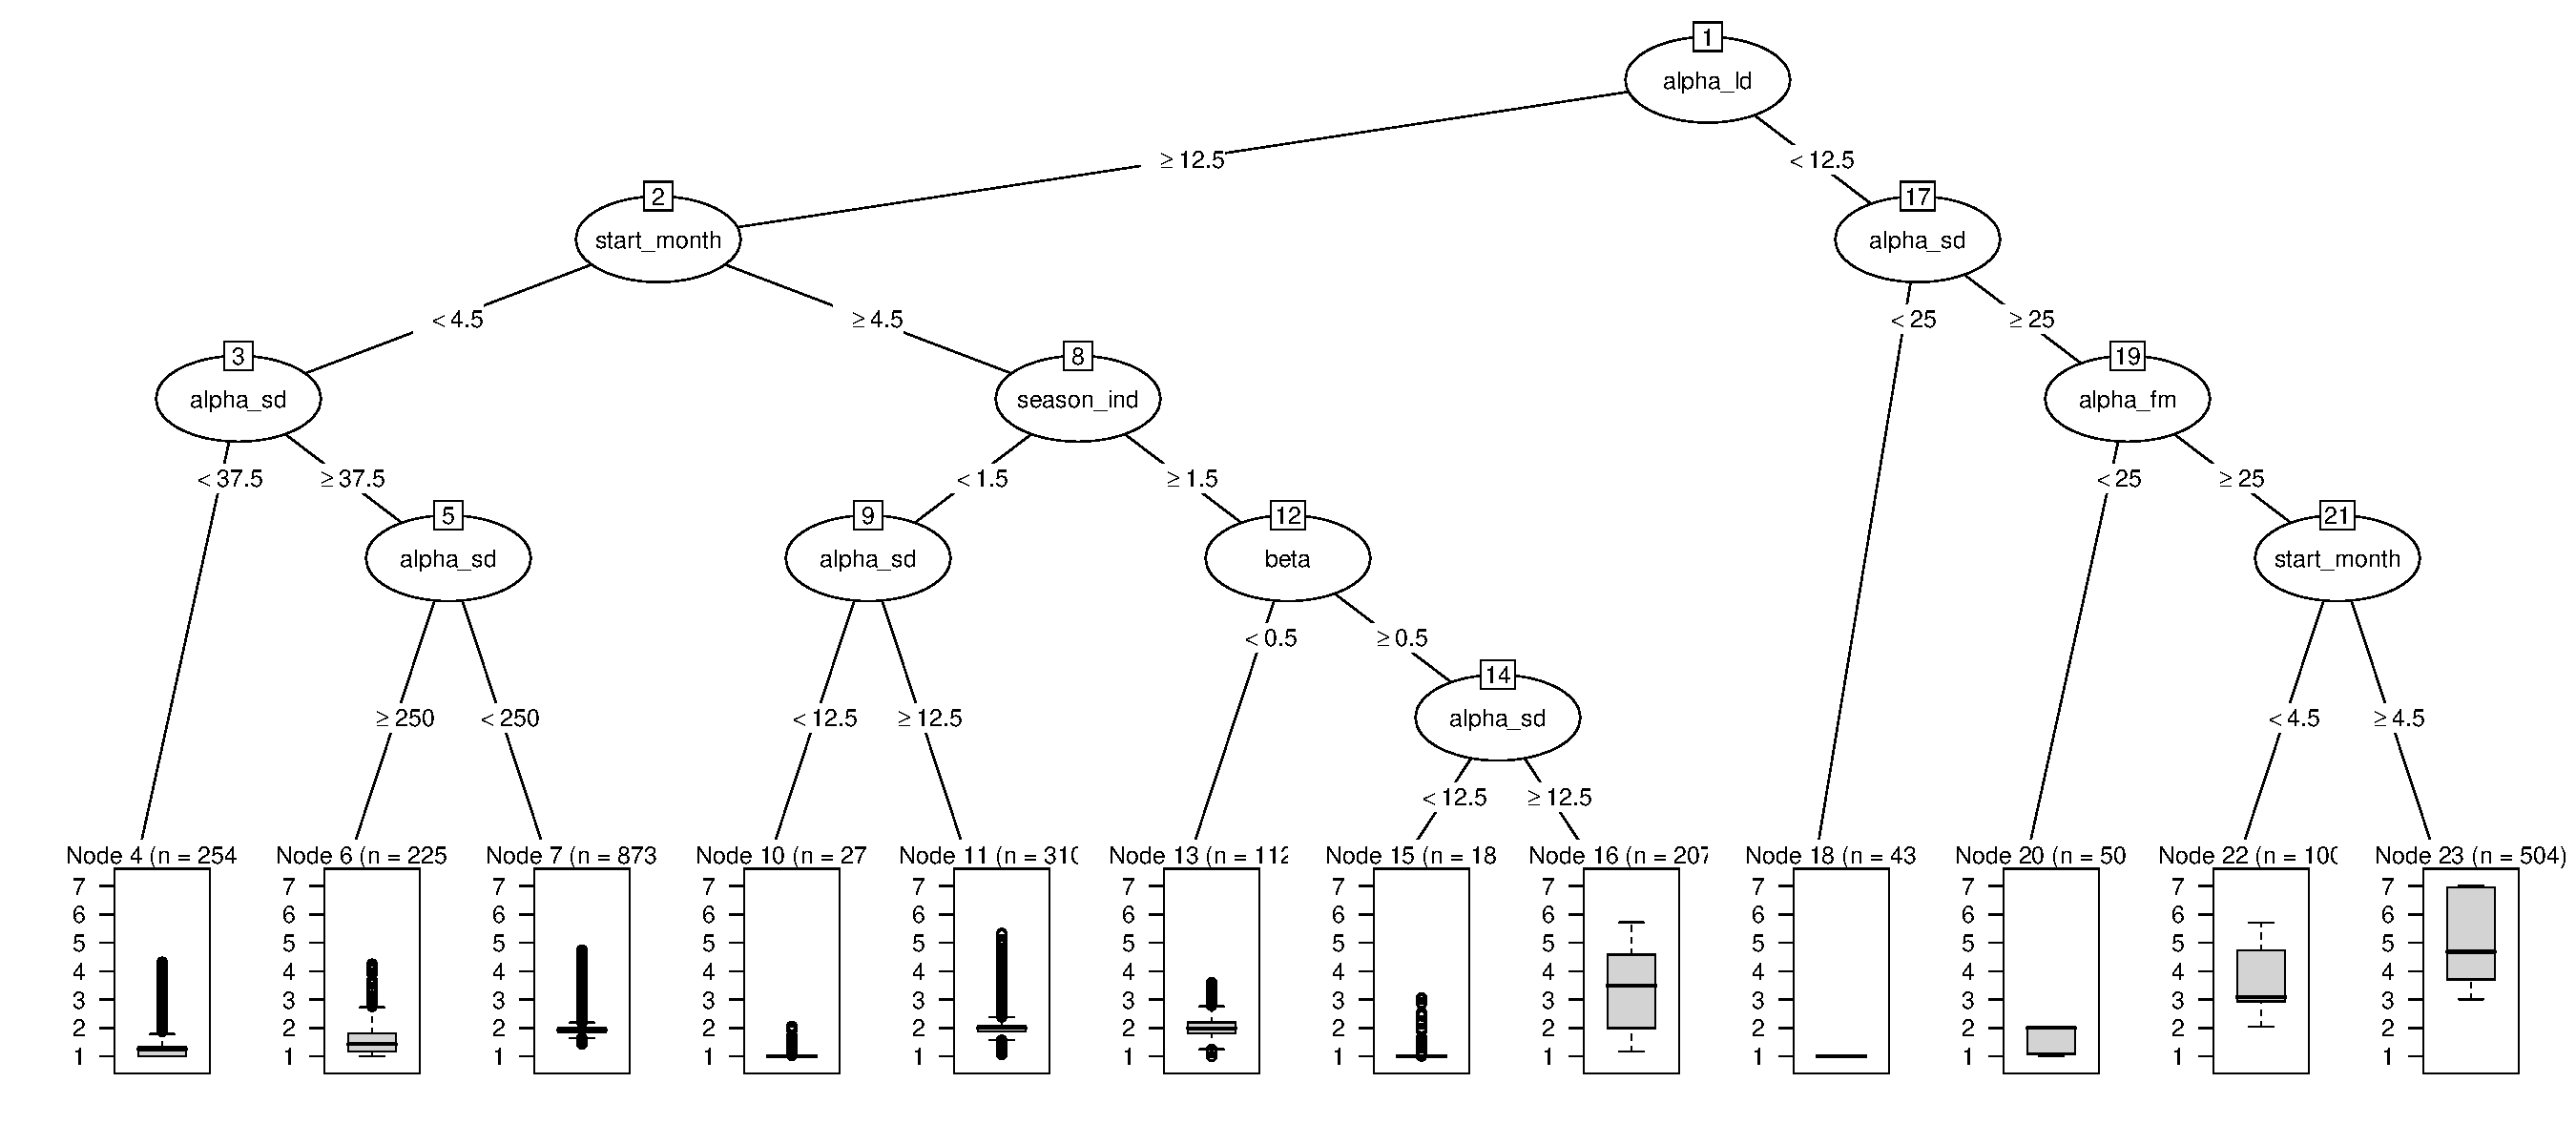
\includegraphics[width=\textwidth,trim={1cm 1cm 1cm 0cm},clip]{../cellular_automata/results/cart/m1_l1_tree.pdf}
\caption{$\mooreRange=1$, $\ell=1$}
    \end{subfigure}
    \begin{subfigure}[b]{.45\textwidth}
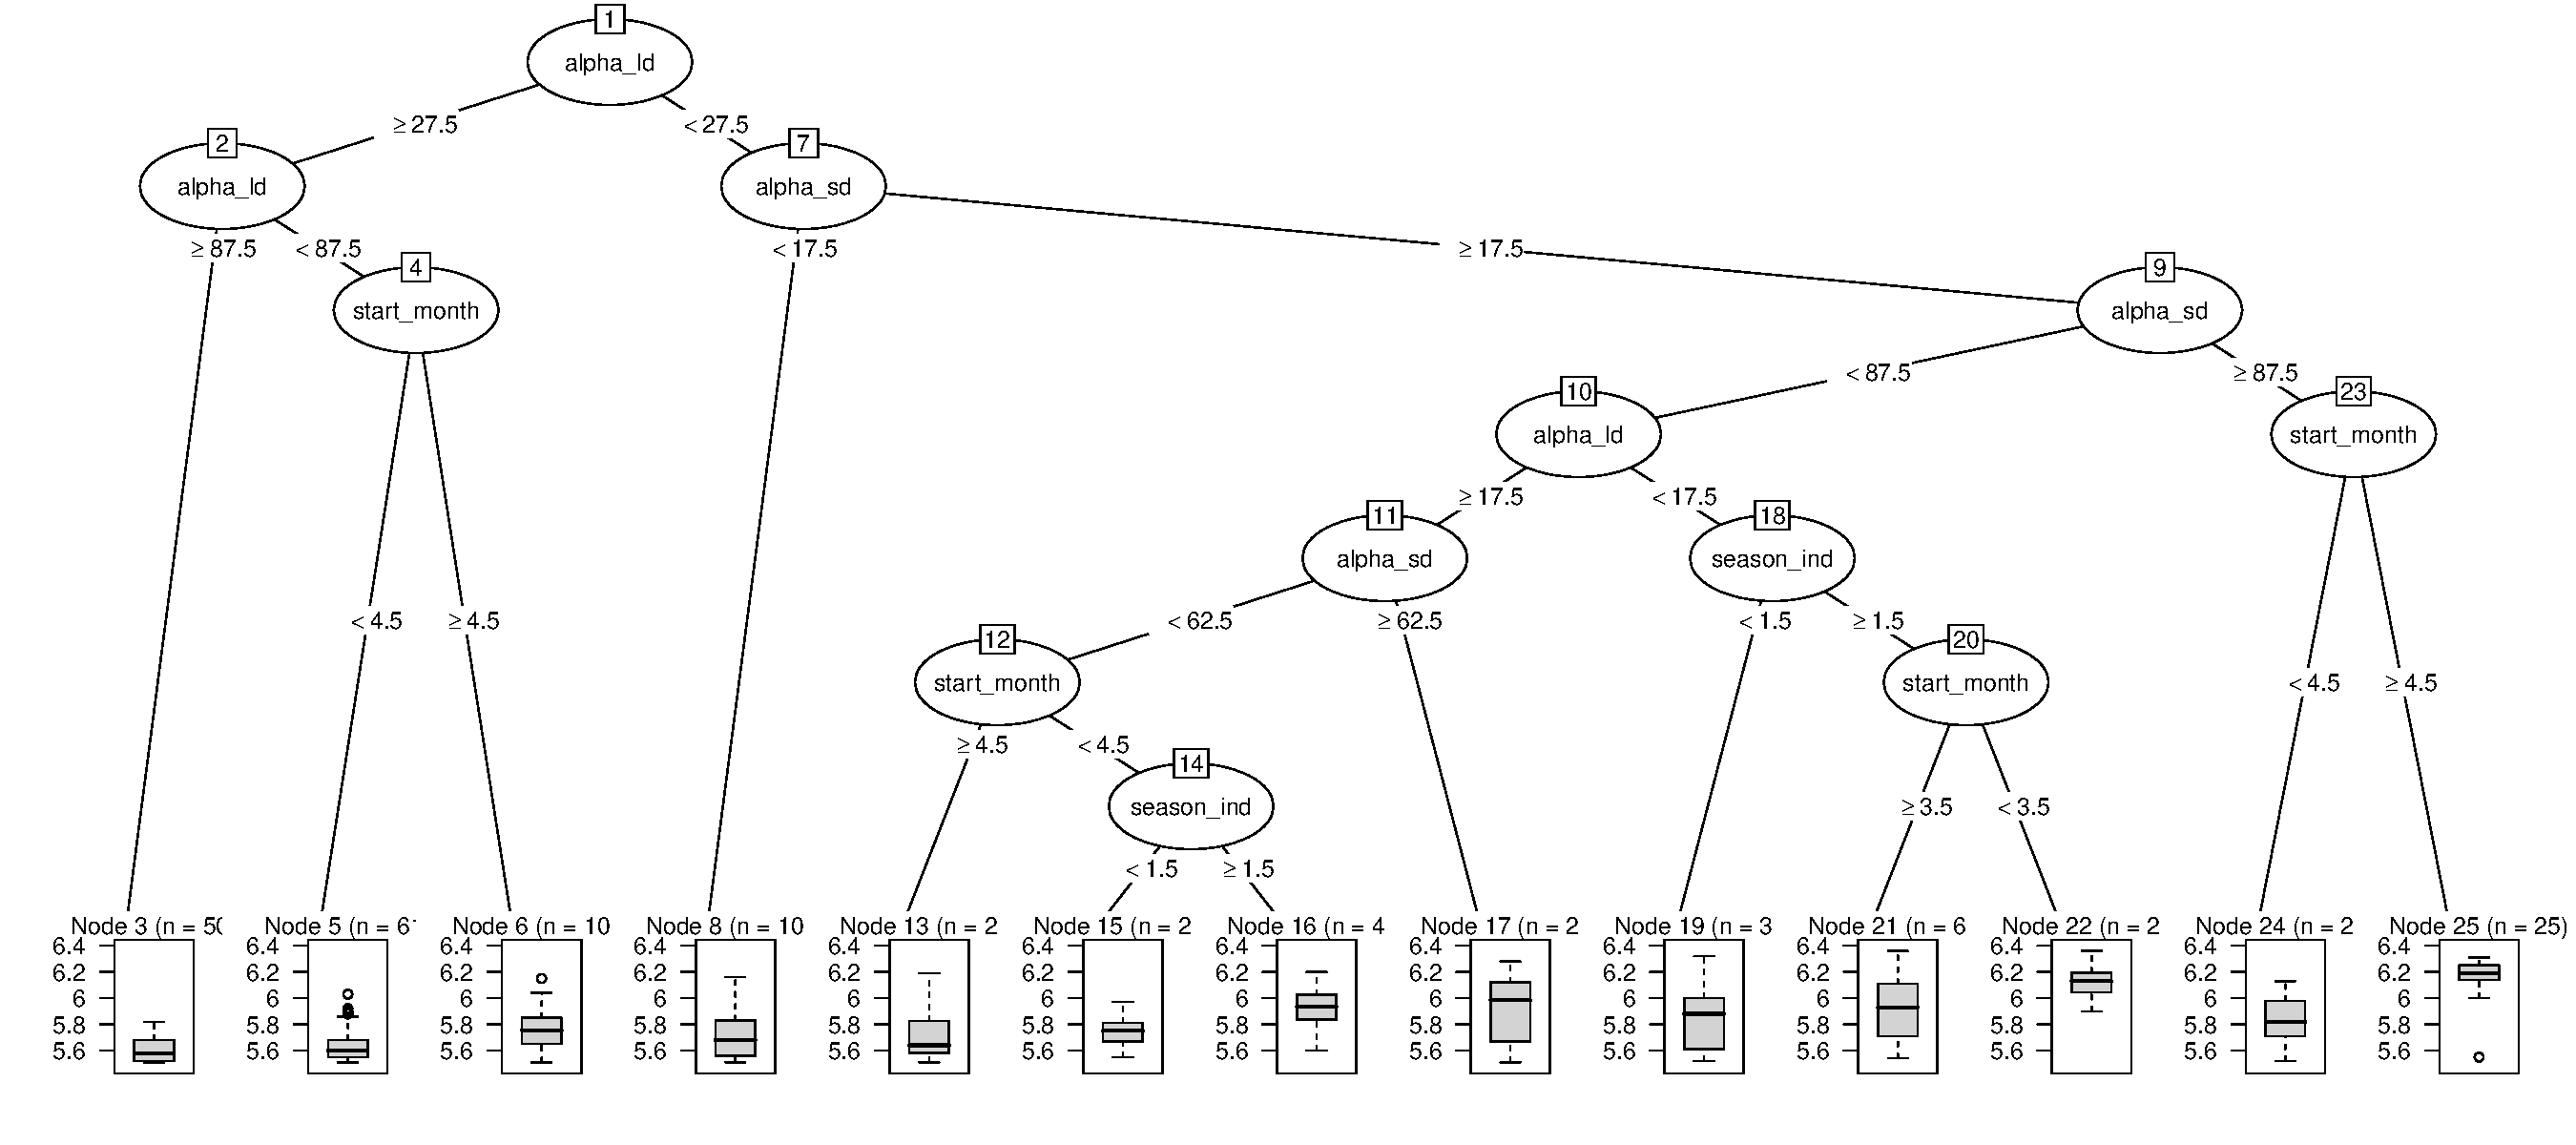
\includegraphics[width=\textwidth,trim={1cm 1cm 1cm 0cm},clip]{../cellular_automata/results/cart/m1_l2_tree.pdf}
\caption{$\mooreRange=1$, $\ell=2$}
    \end{subfigure}
    \begin{subfigure}[b]{.45\textwidth}
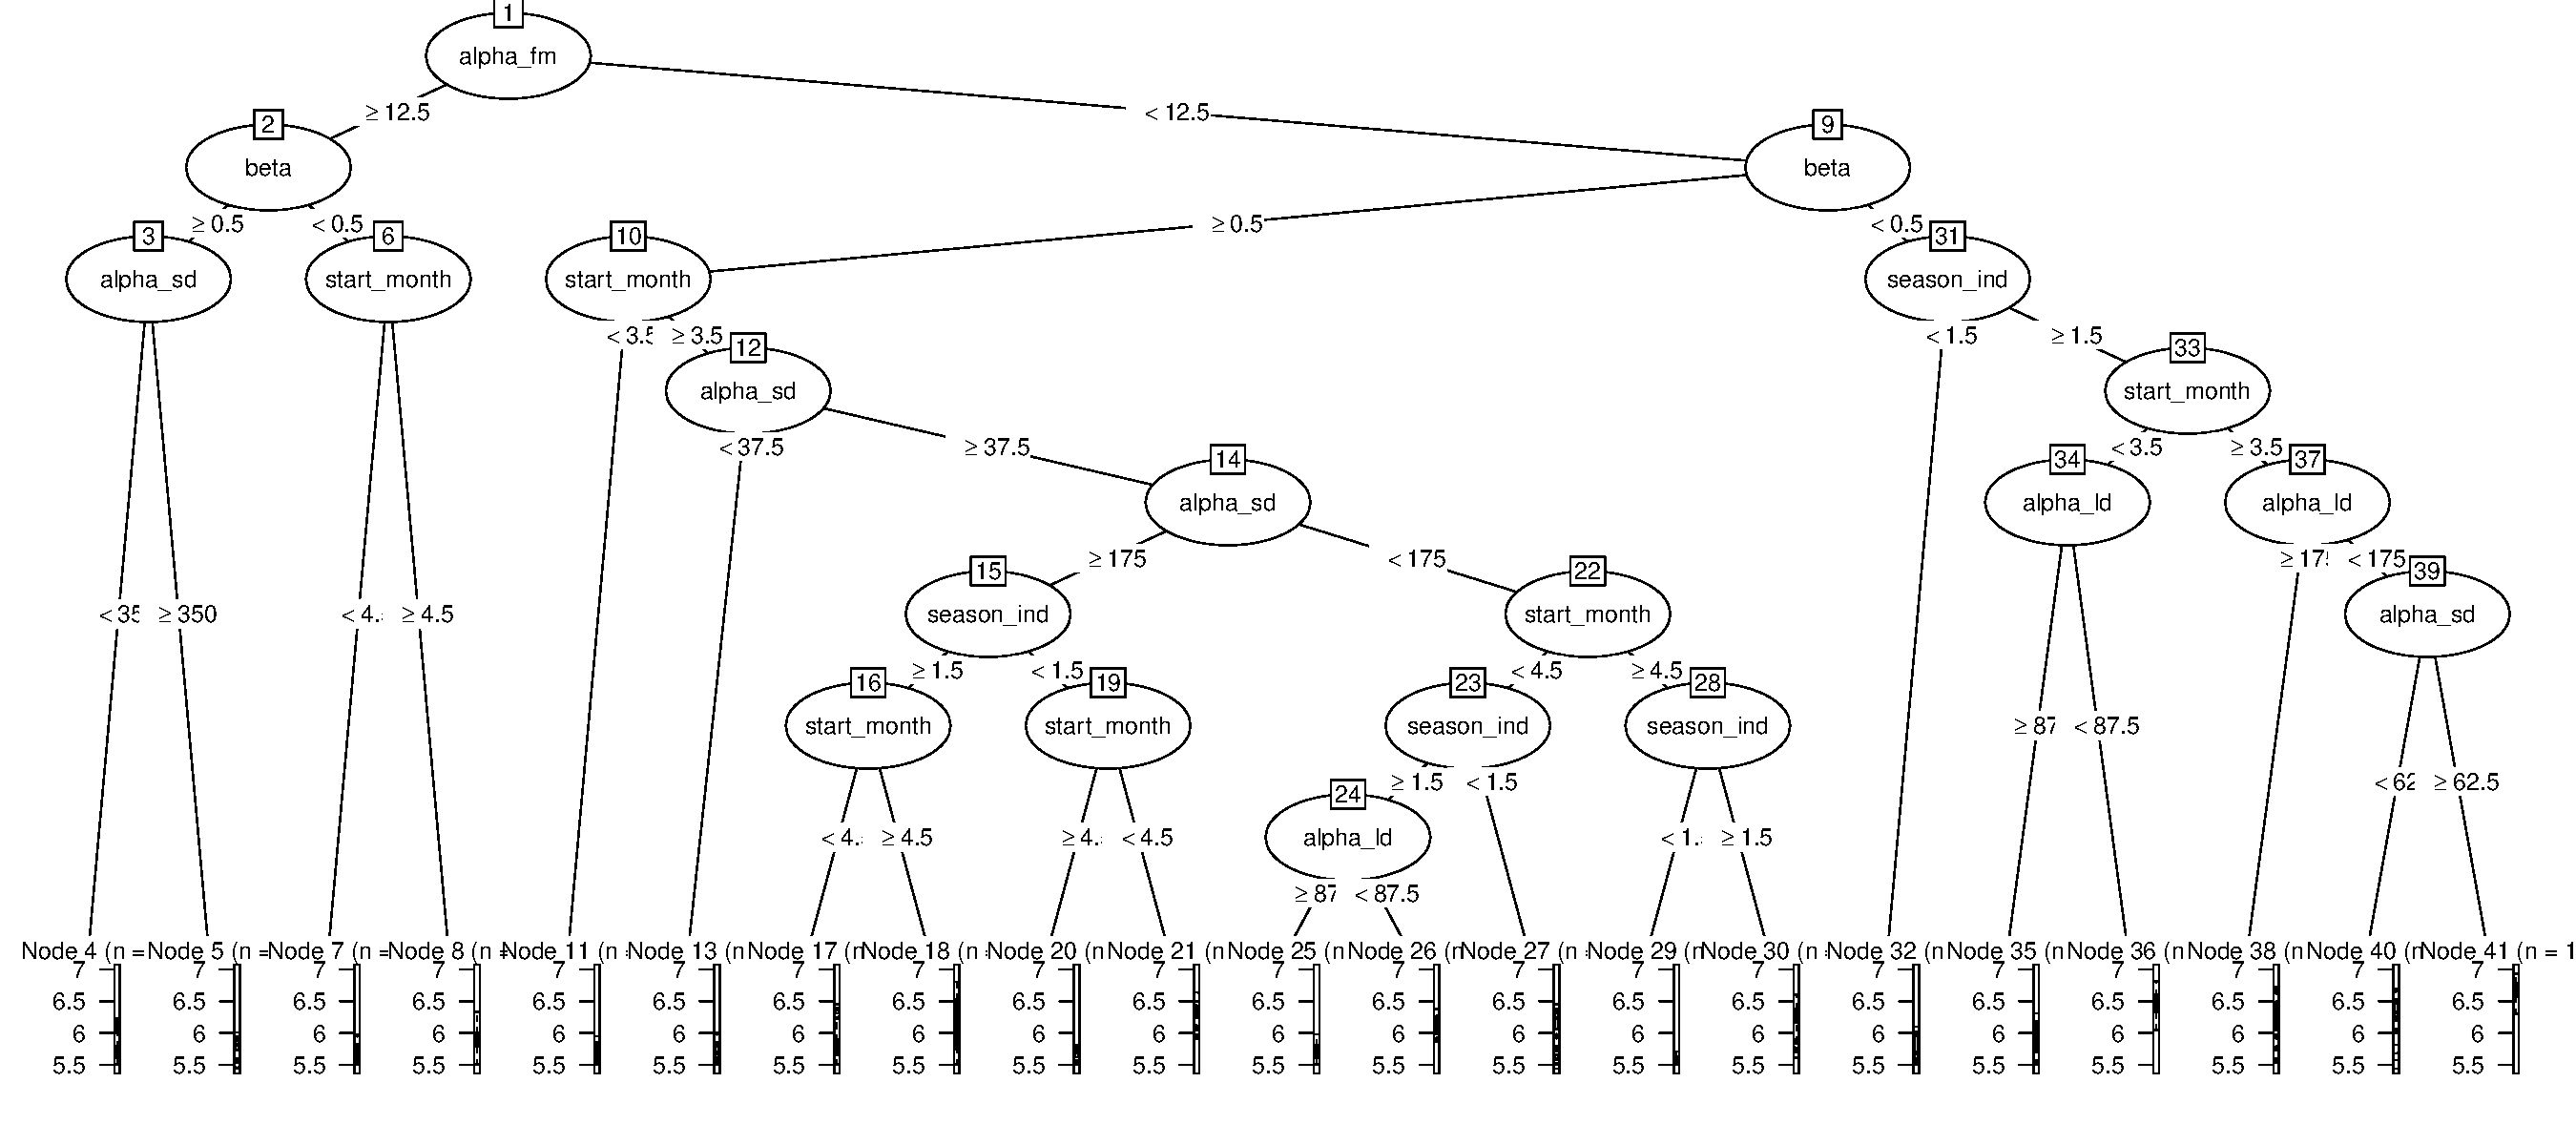
\includegraphics[width=\textwidth,trim={1cm 1cm 1cm 0cm},clip]{../cellular_automata/results/cart/m1_l3_tree.pdf}
\caption{$\mooreRange=1$, $\ell=3$}
    \end{subfigure}
    \begin{subfigure}[b]{.45\textwidth}
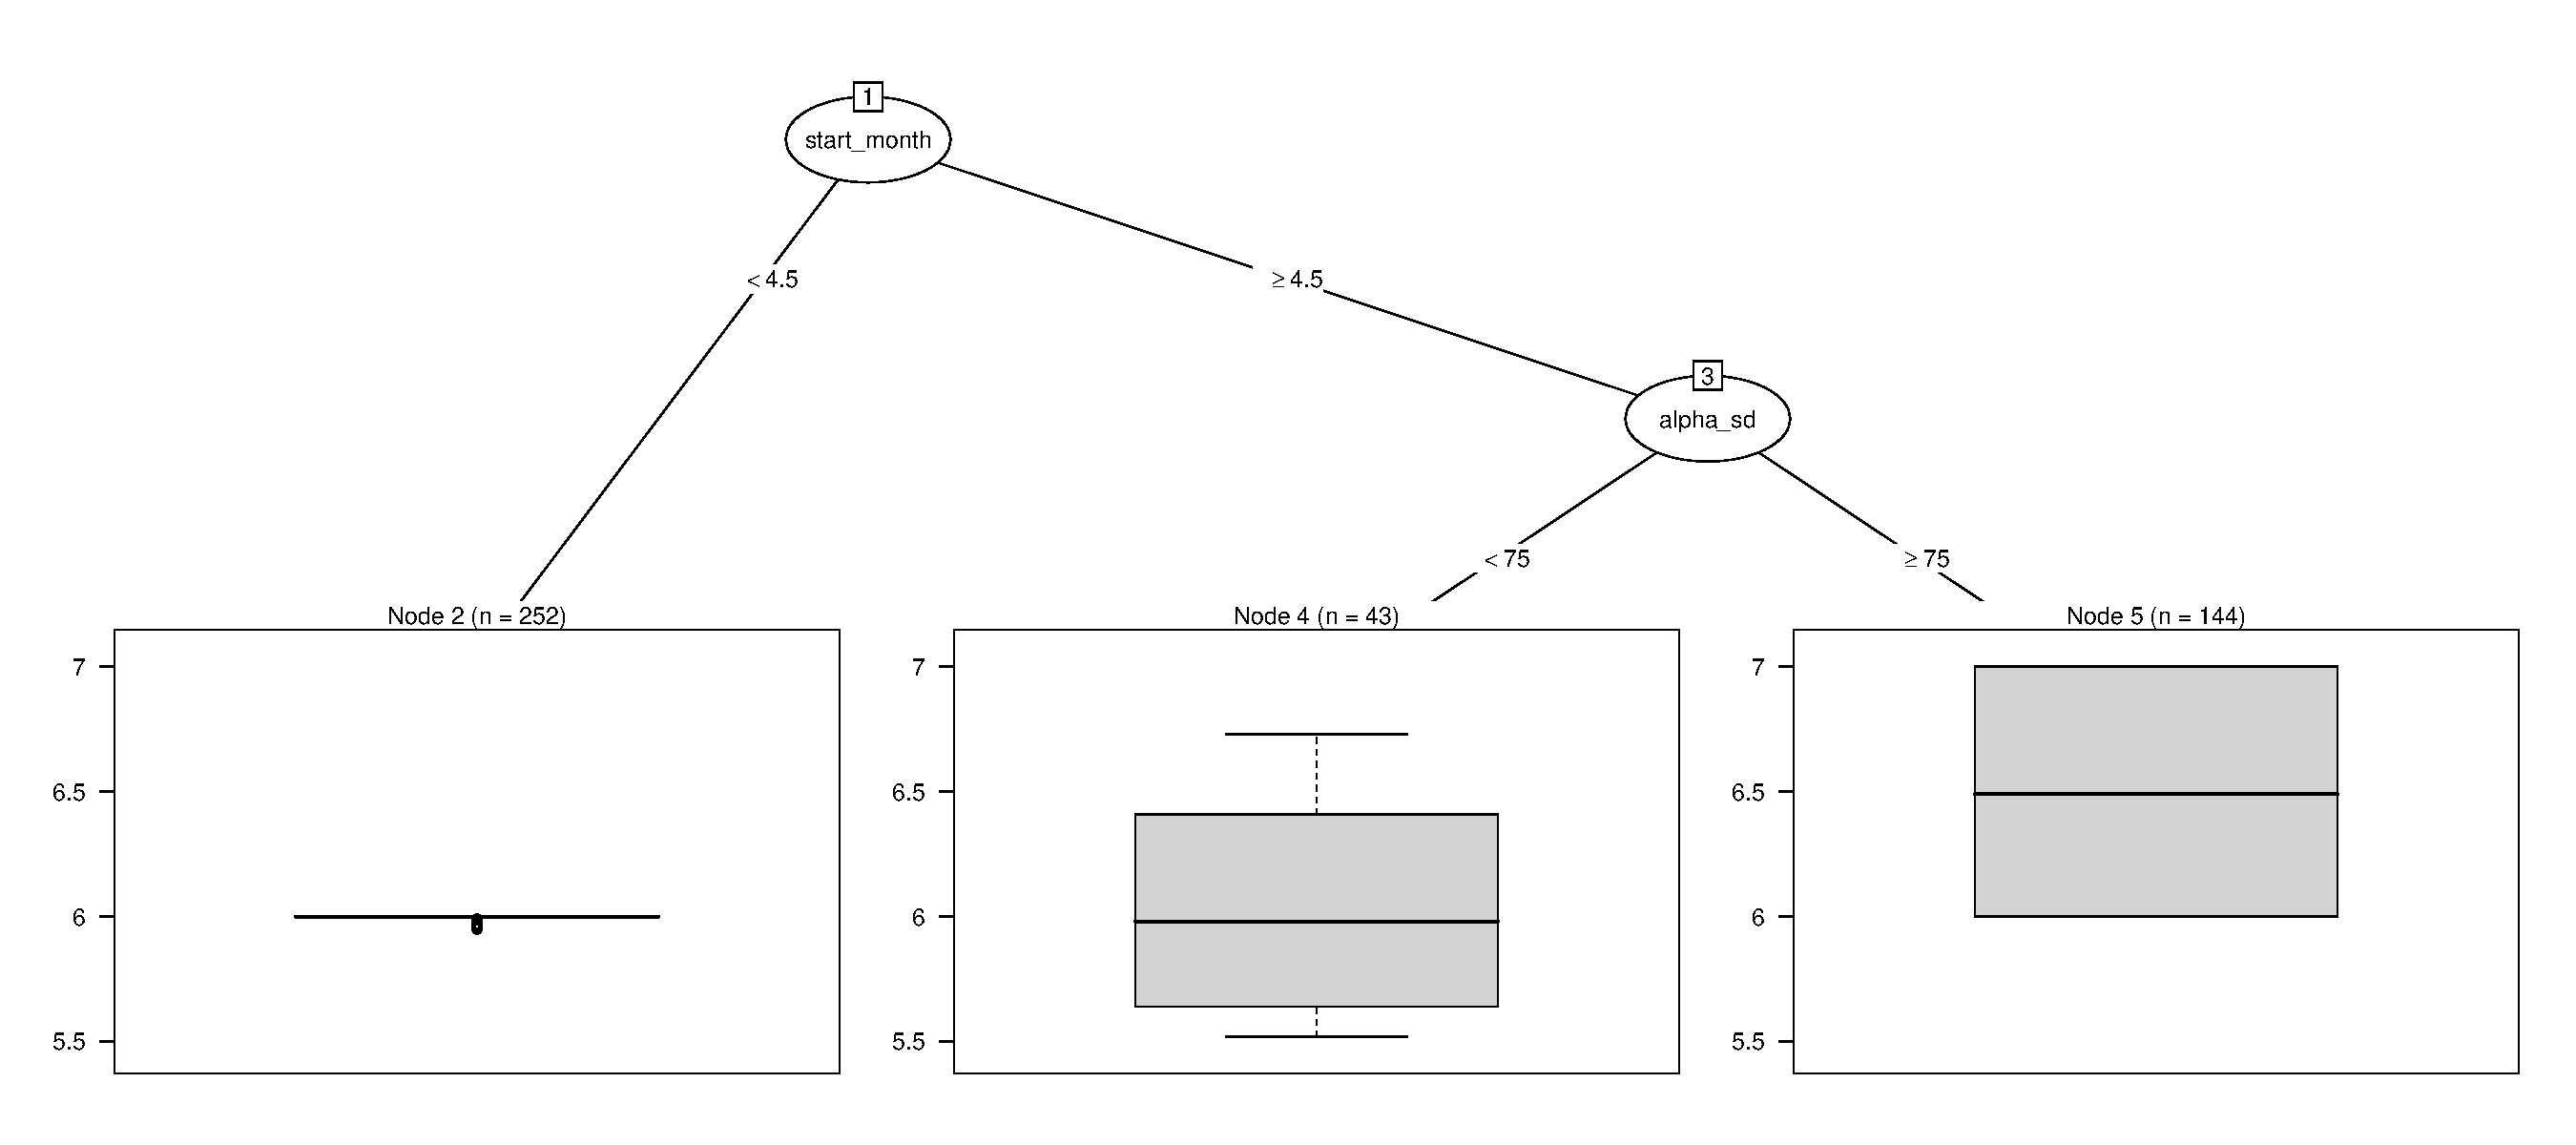
\includegraphics[width=\textwidth,trim={1cm 1cm 1cm 0cm},clip]{../cellular_automata/results/cart/m2_l1_tree.pdf}
\caption{$\mooreRange=2$, $\ell=1$}
    \end{subfigure}
    \begin{subfigure}[b]{.45\textwidth}
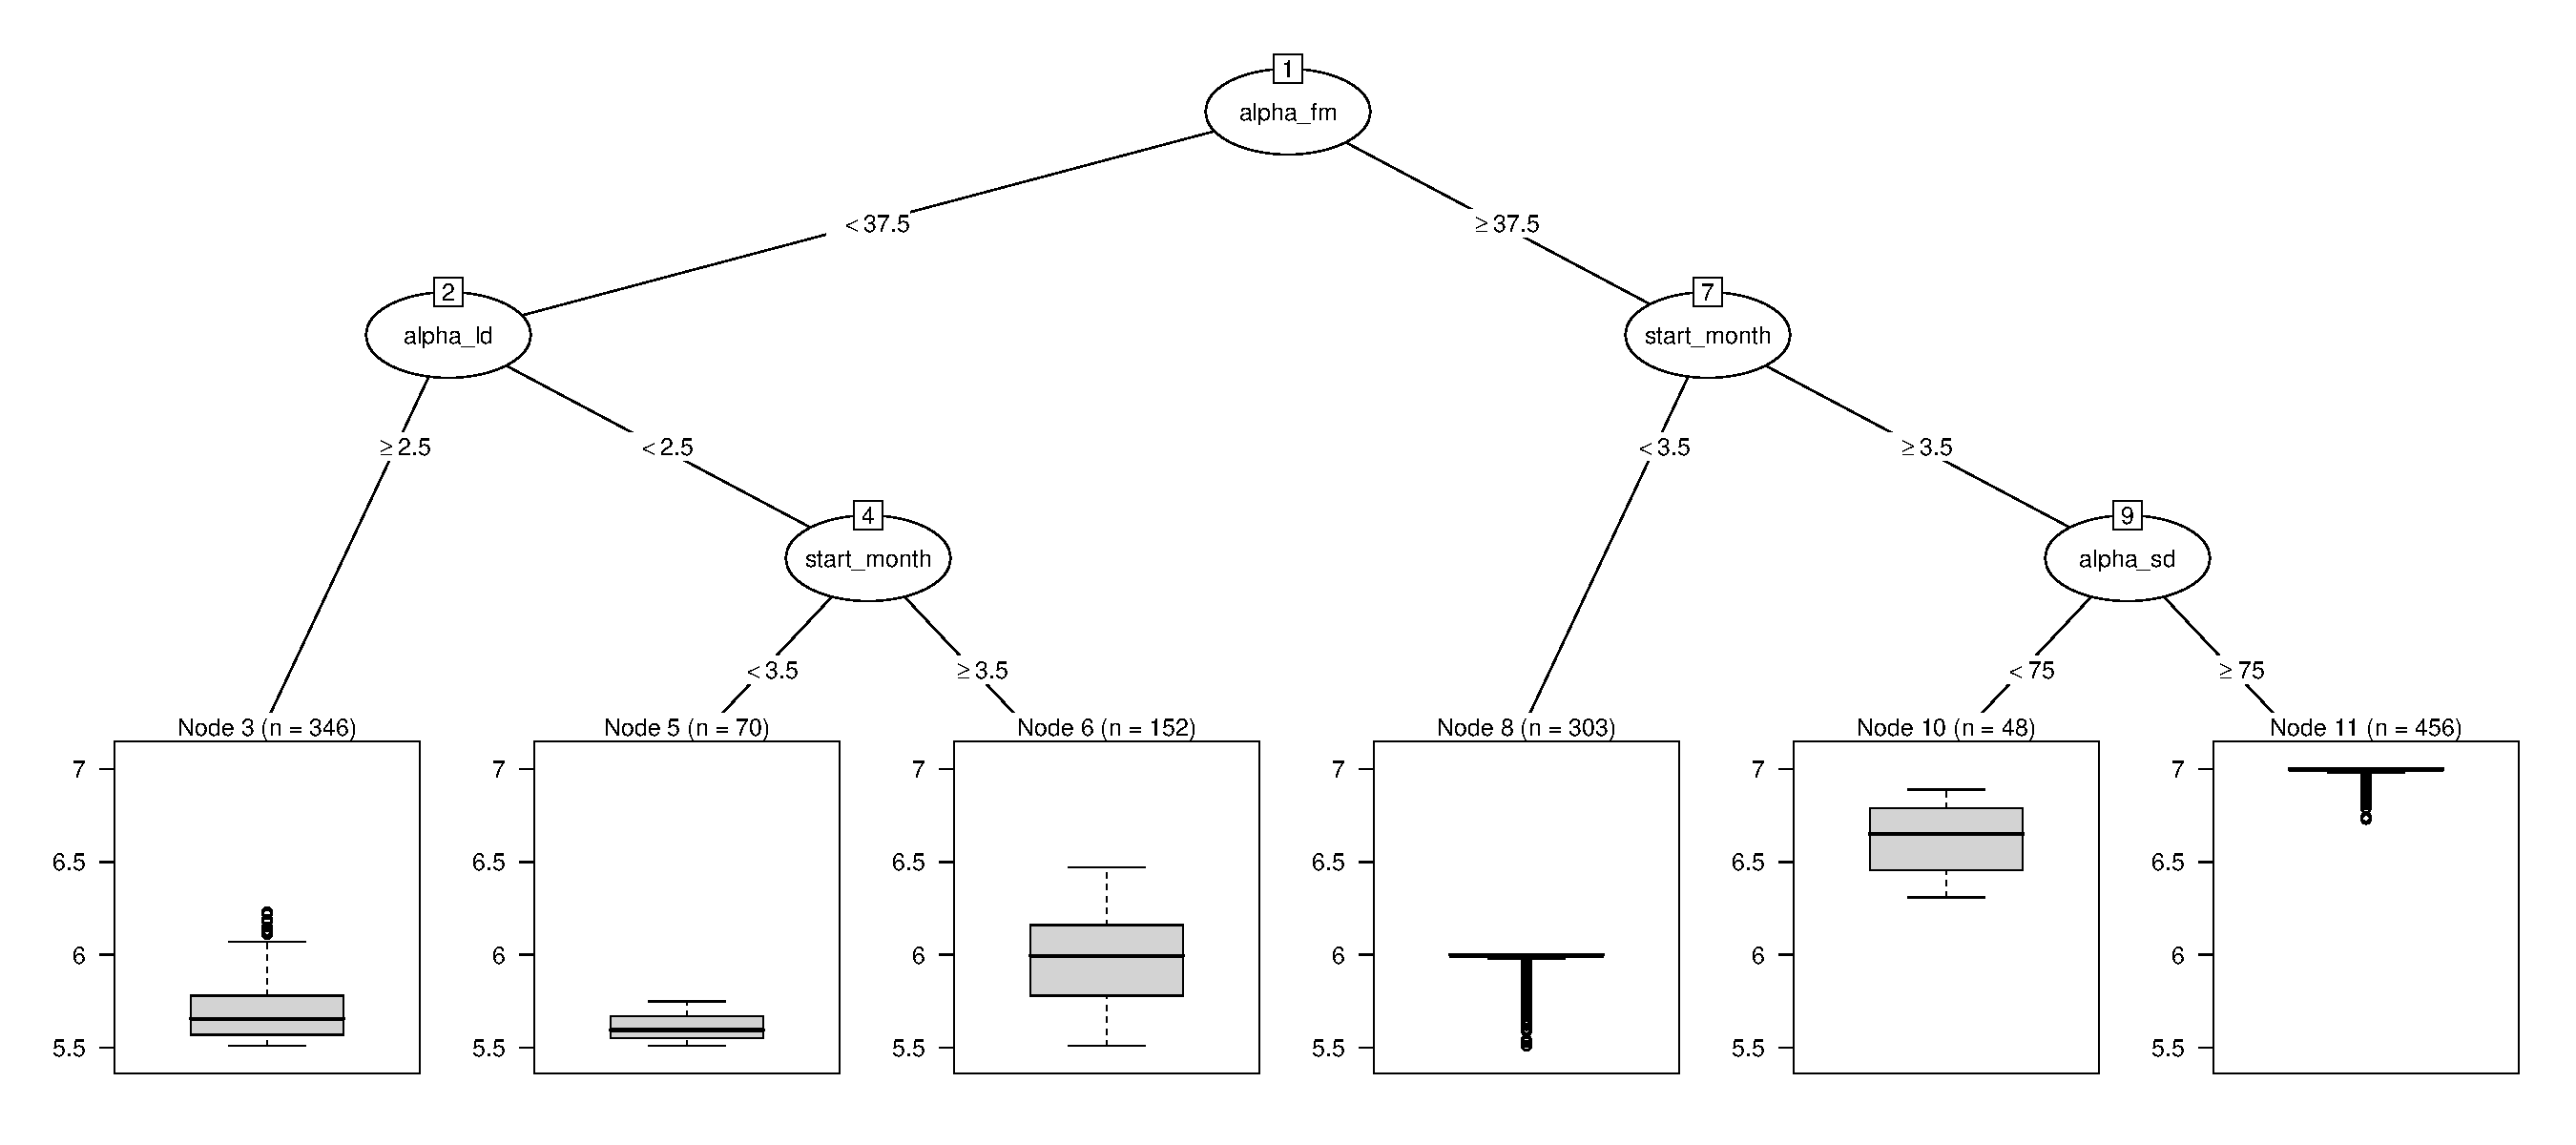
\includegraphics[width=\textwidth,trim={1cm 1cm 1cm 0cm},clip]{../cellular_automata/results/cart/m2_l2_tree.pdf}
\caption{$\mooreRange=2$, $\ell=2$}
    \end{subfigure}
    \begin{subfigure}[b]{.45\textwidth}
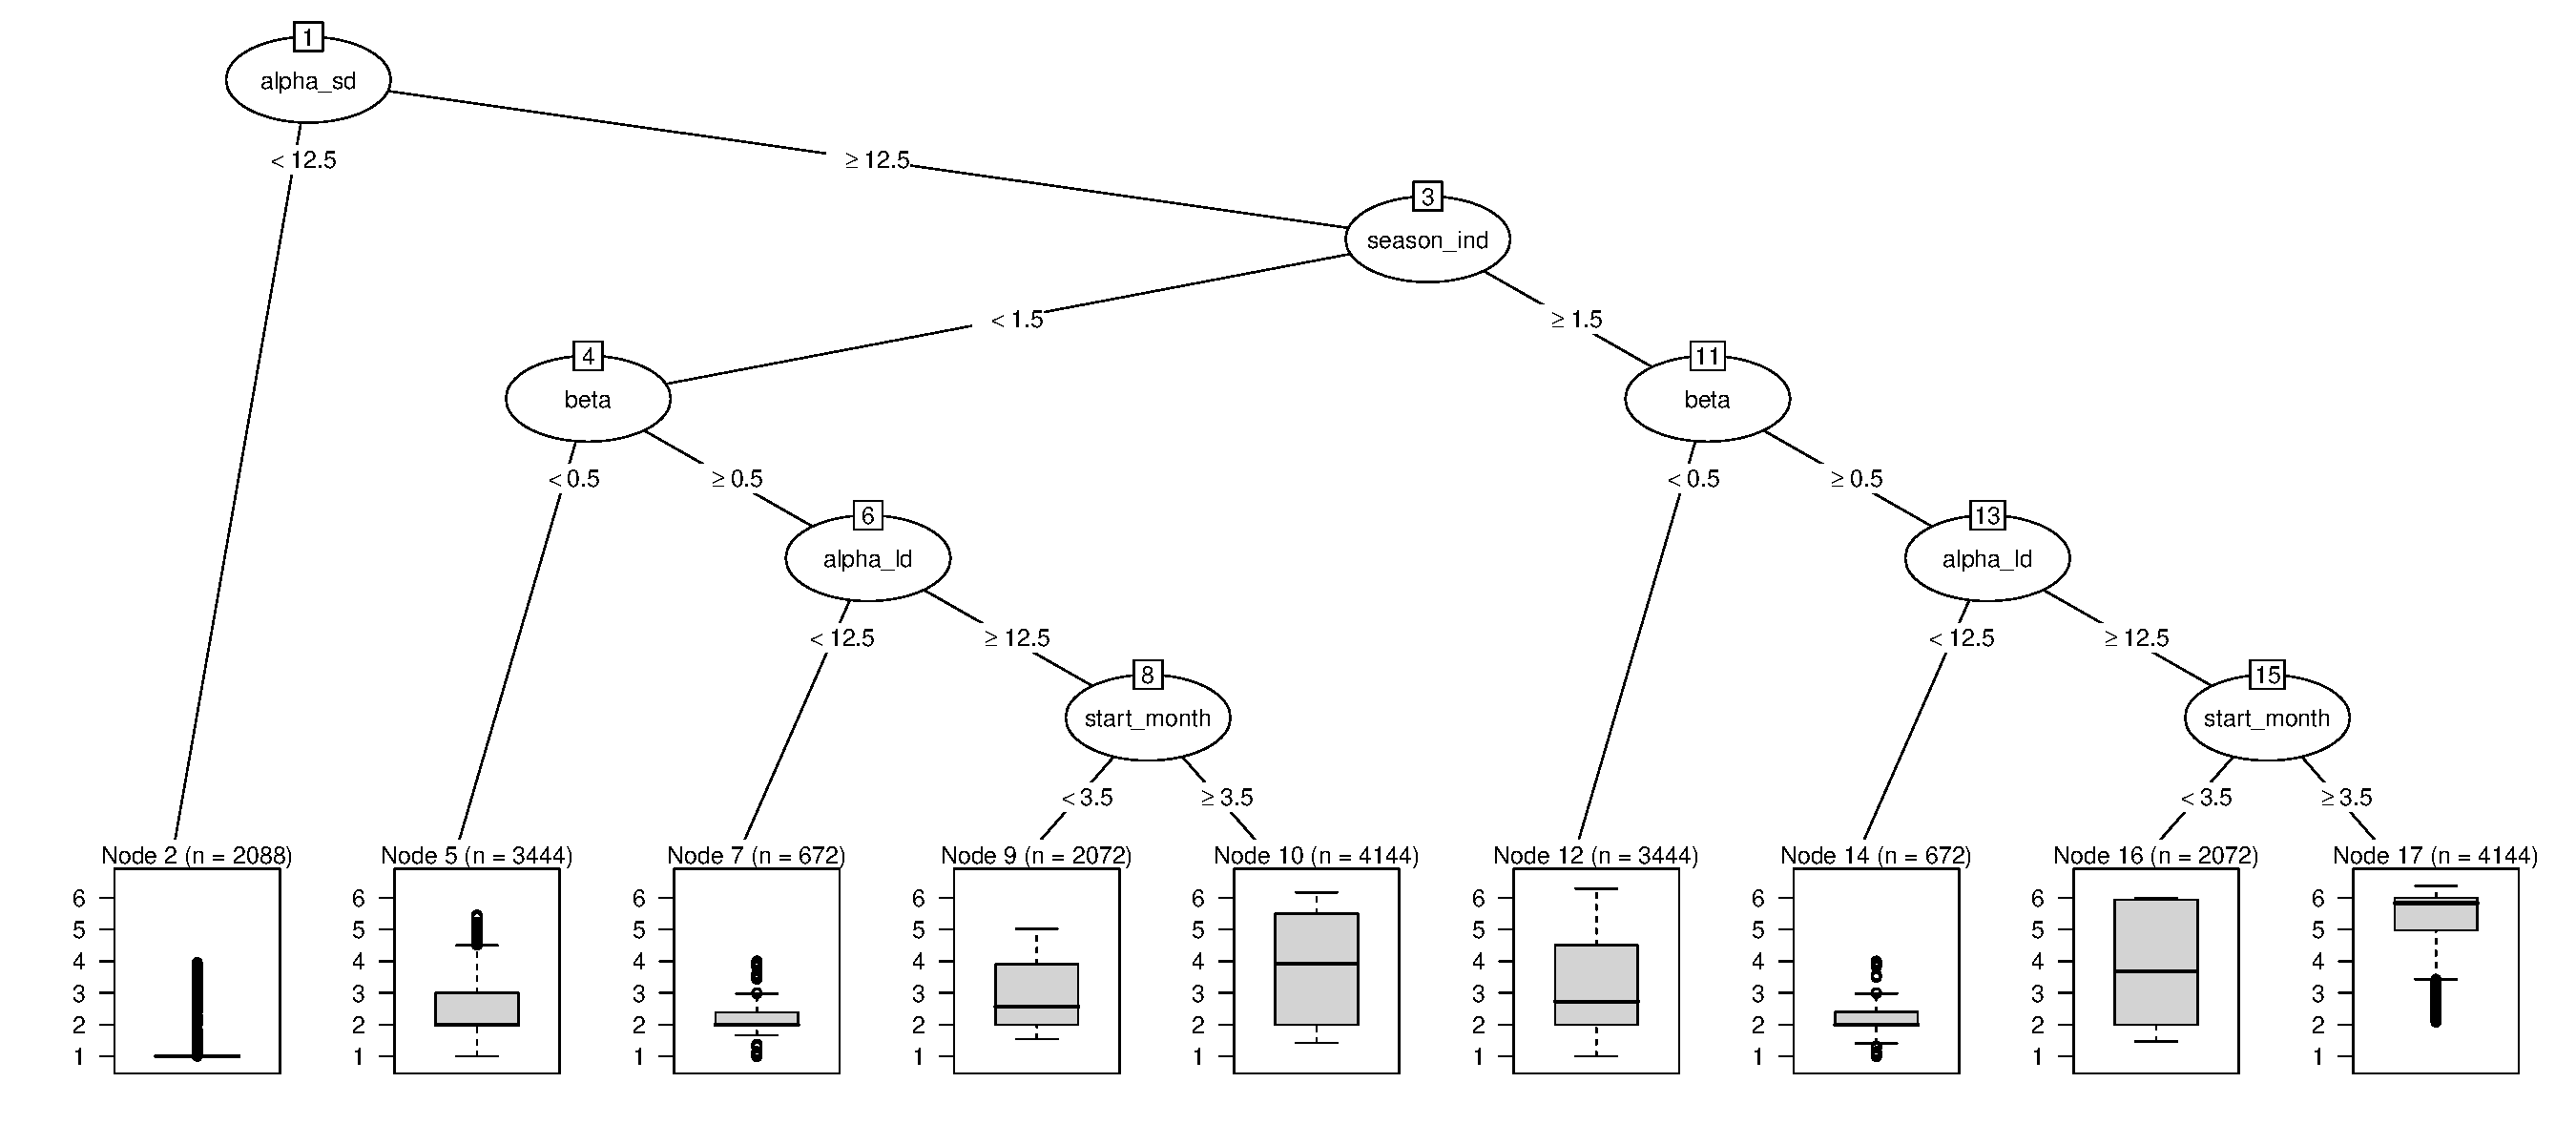
\includegraphics[width=\textwidth,trim={1cm 1cm 1cm 0cm},clip]{../cellular_automata/results/cart/m2_l3_tree.pdf}
\caption{$\mooreRange=2$, $\ell=3$}
    \end{subfigure}
%%     \begin{subfigure}[b]{.45\textwidth}
%% 
\includegraphics[width=\textwidth,trim={1cm 1cm 1cm 0cm},clip]{../cellular_automata/results/cart/m3_l1_tree.pdf}
%% \caption{$\mooreRange=3$, $\ell=1$}
%%     \end{subfigure}
    \begin{subfigure}[b]{.45\textwidth}
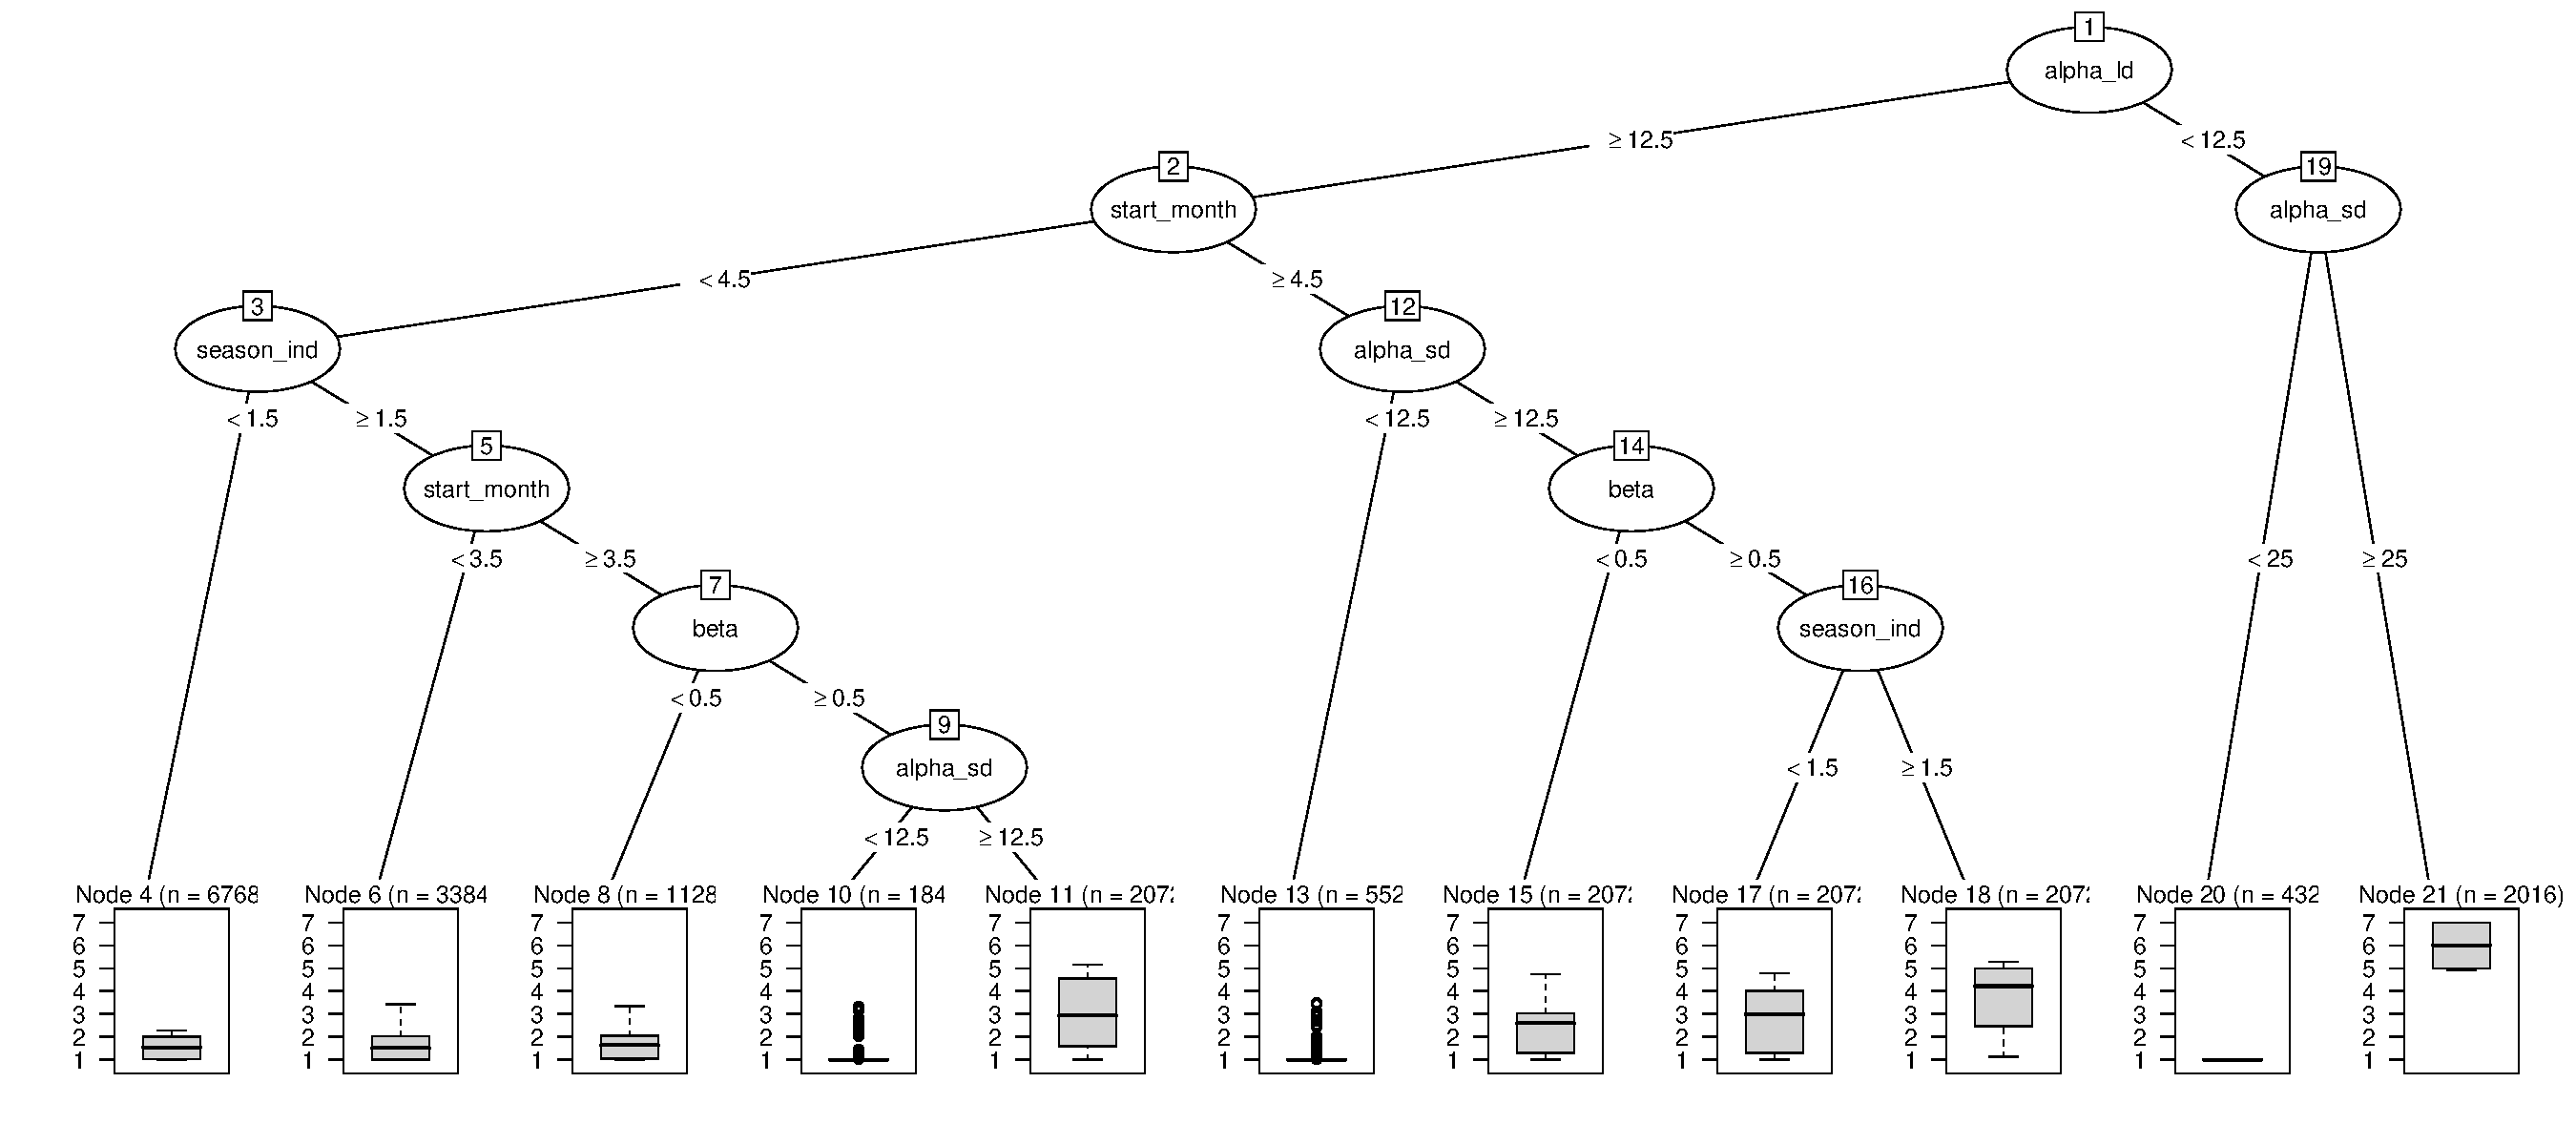
\includegraphics[width=\textwidth,trim={1cm 1cm 1cm 0cm},clip]{../cellular_automata/results/cart/m3_l2_tree.pdf}
\caption{$\mooreRange=3$, $\ell=2$}
    \end{subfigure}
    \begin{subfigure}[b]{.45\textwidth}
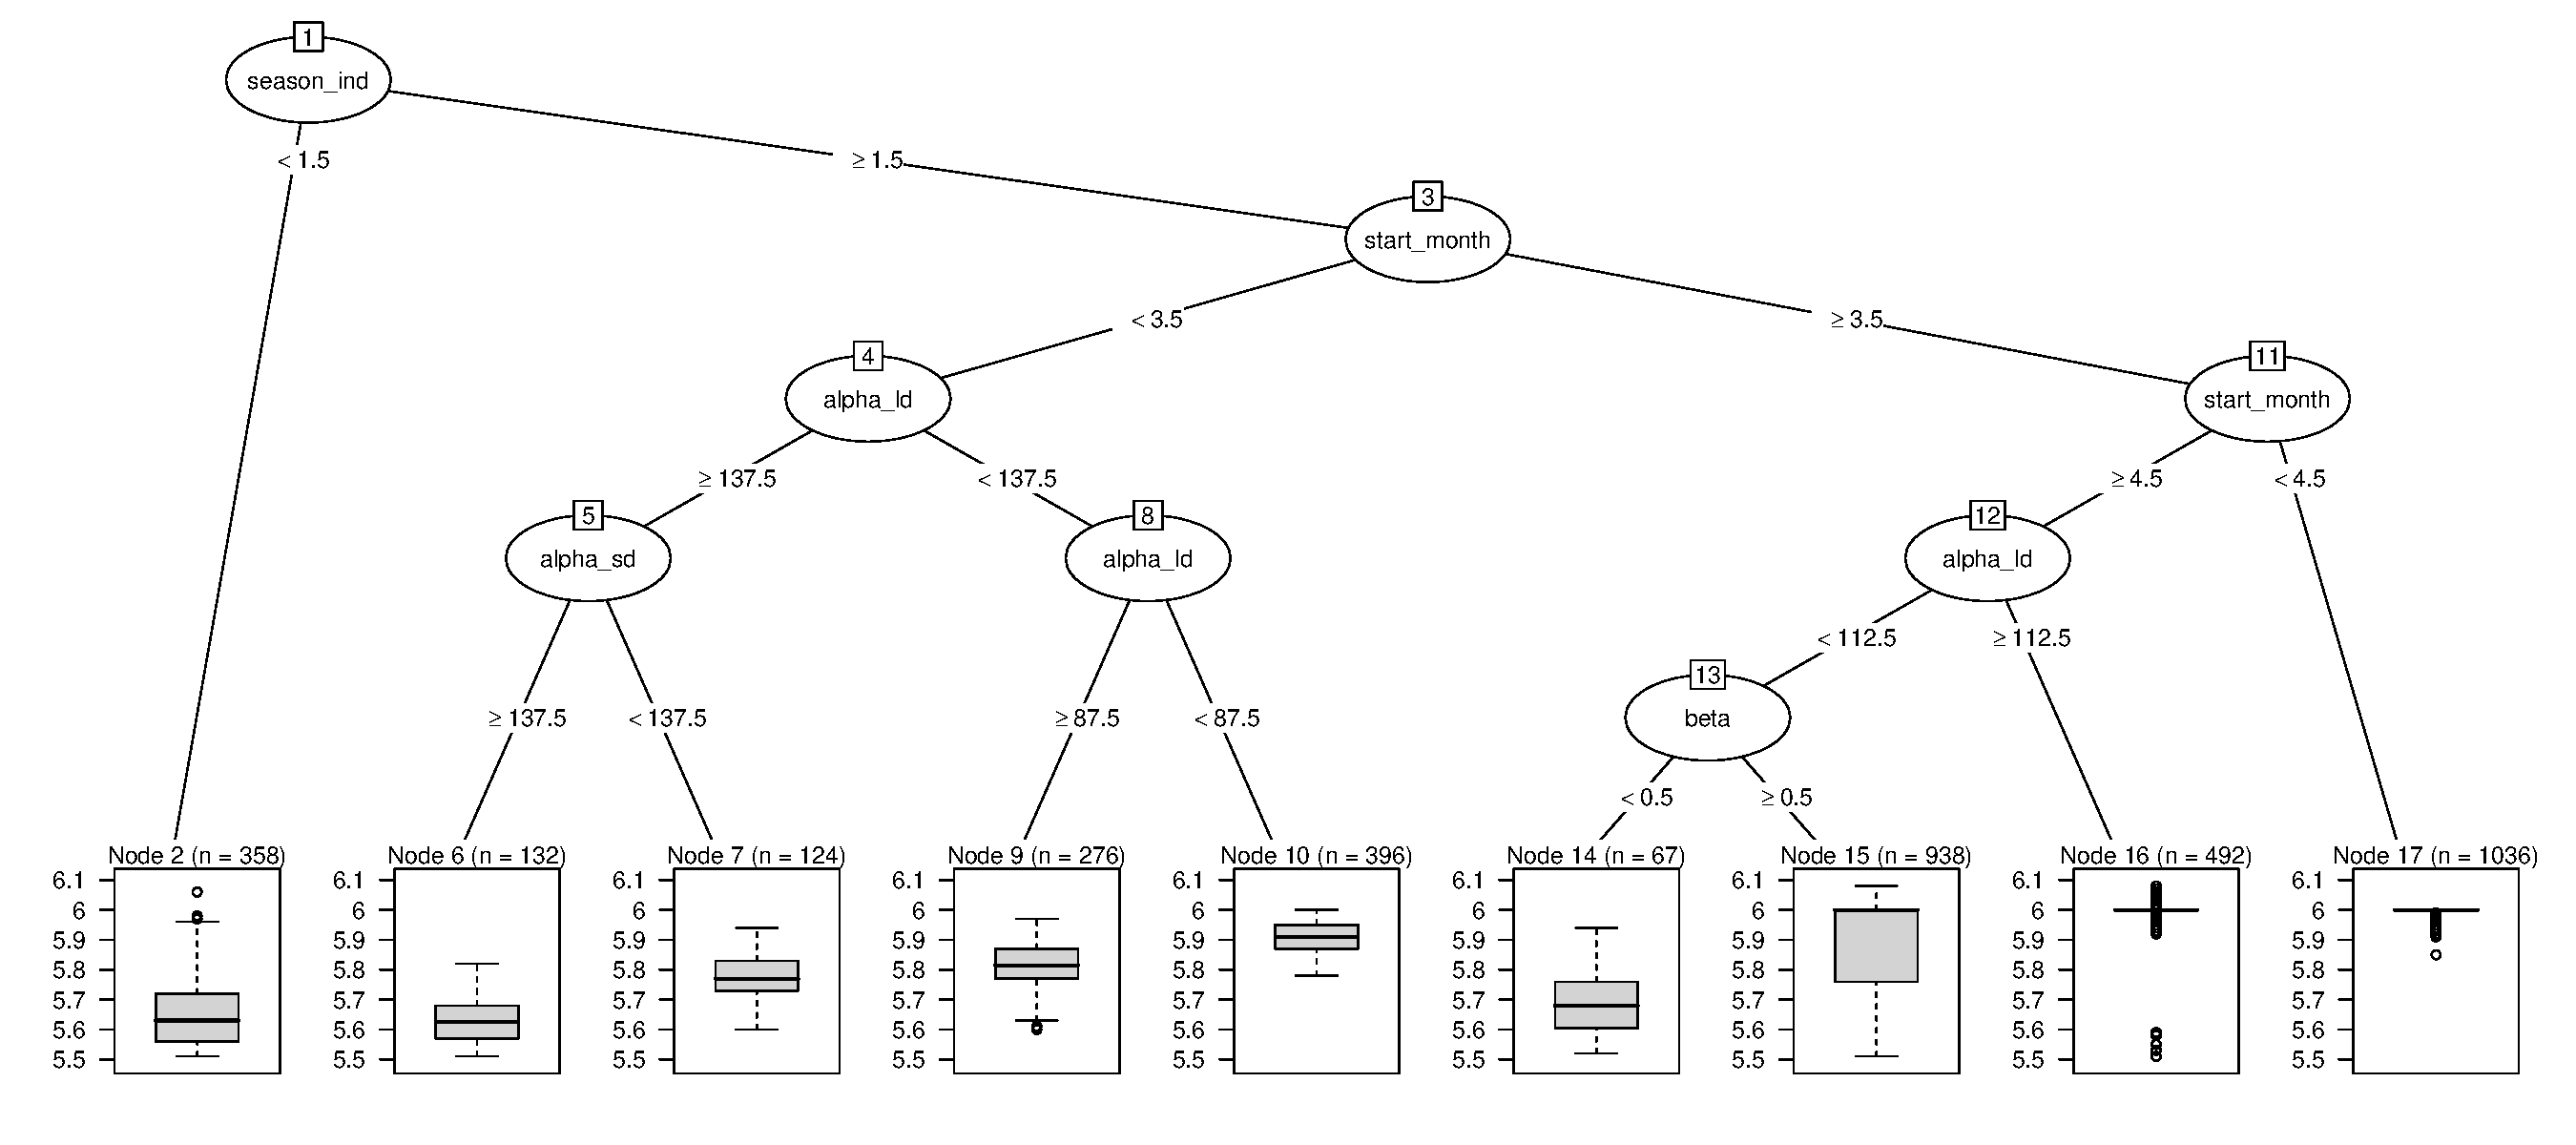
\includegraphics[width=\textwidth,trim={1cm 1cm 1cm 0cm},clip]{../cellular_automata/results/cart/m3_l3_tree.pdf}
\caption{$\mooreRange=3$, $\ell=3$}
    \end{subfigure}
    \caption{CART analysis of the parameter space: The models with
        likelihood~$\ge5.5$ were partitioned based on the Moore
    range~$\mooreRange$ and latency period~$\ell$ tuple and analyzed. For
 the case~$(\mooreRange=3$, $\ell=1)$, there were no instances with
 likelihood~$\ge5.5$ among the sampled instances. 
    \label{fig:cart}}
\end{figure}

We recall that the emergent outcome of the model can be classified into two
classes: Class~A and Class~B. In Figure~\ref{fig:cart}, we show the results
of CART analysis on the parameter sets which yielded a likelihood of
$\ge5.5$. The chosen set is partitioned by Moore range~$\mooreRange$ and
latency period~$\ell$. For $(\mooreRange,\ell)$ values that permit rapid
range expansion through short-distance spread over the contiguous
landscape, including long-distance spread leads to faster spread than
observed leading to lower likelihood values. Hence, for those regimes, we
observe only Class~A spread. The corresponding~$(\mooreRange,\ell)$ values
are~$(1,1)$, $(2,1)$, $(2,2)$ and $(3,1)$. For the regime~$(3,1)$ we did
not observe any instance with likelihood~$>5.5$.

\subsection{Seeding scenarios}
\label{tab:seeds}
During the model evaluation phase, to account for both spatial and temporal
observation noise, we considered six seeding scenarios: The locations
Bangladesh~1 and Bangladesh~2 (see Table~\ref{tab:seeds}) and start times
March, April or May (the month \tuta{} was reported).  For the prediction
phase, we constructed three different seeding scenarios reflecting three
different possible introductions to the region. The first corresponds to
spread from Bangladesh through northeast Myanmar. This region represents a
possible pathway of \tuta{} should it spread radially through the border
with Bangladesh. The second scenario we considered is the region of Johor
in Malaysia - including Singapore. This region contains major ports in
Malaysia including Tanjung Pelepas \cite{khalid2005}, and Singapore is also
a major trading hub for Bangladesh. We considered two scenarios of
introduction for Philippines. The first is motivated by the fact that there
is a large migrant Filipino worker population traveling to and from
infested countries. We seeded the port of Masinloc in this scenario as it
processes many of these travelers. The second was the introduction to
Northern Mindanao region, one of the major tomato production areas in the
country. We conducted country-specific experiments in the case of Thailand
and Vietnam. The seed locations were determined by spread observed from
both Class~A and Class~B models.
%% Scenario C seeded the region of
%% Putrajaya, which is the region which includes the largest port in Malaysia
%% \cite{khalid2005}. Scenario D seeded the region of Penang, which is also a
%% major port \cite{khalid2005}. 
%% Scenario E seeded Sarawak which is one of the
%% Malaysia districts not in the mainland. This district contains another
%% major port: Bintulu \cite{khalid2005}. When seeded in the mainland, the
%% Sarawak region is not reached with a Moore range of 2 or 3.This reflects
%% the natural spread of \tuta{} across the border of Myanmar. In this case we
%% seeded all cells northeast of a given boundary line, this is due to
%% uncertainty of the current distribution of the pest as well as likely
%% movement. The second scenario is an introduction through Singapore due to
%% trade. 
%%
\begin{table}[ht]
    \caption{Seeding scenarios\label{tab:seed}}
    \centering
    \small
    \begin{tabular}{p{4cm} p{10cm}}
    	\hline
    	Region seeded & Description \\
    	\hline
    	\hline
        Bangladesh 1 & Parameterization phase: The cell corresponding to the location of first
        report was seeded. \\
        Bangladesh 2 & Parameterization phase: The cells corresponding to the location of first
        report and its adjacent cells were seeded. \\
    	\hline
	Bangladesh and Northeastern Myanmar & This seeding is the estimated
	current range of \tuta{} in the study region. It is used to study
	the spread in the rest of the region.\\
    	\hline
    	Singapore and southern (mainland) Malaysia & This reflects possible introduction through trade, as Singapore is a major port.\\
    	\hline
    	Philippines 1 & This reflects the possibility of \tuta{} being
        introduced through workers traveling to and from India, and other
        countries, which have reported the pest. The port of Masinloc was
        seeded.\\
    	Philippines 2 & Northern Mindanao region\\
    	Thailand & Northwestern region: informed by observed spread in
        Mainland Southeast Asia.\\
    	Vietnam & Northwester region: Informed by observed spread in
        Mainland Southeast Asia.\\
    	\hline
    	\end{tabular}
\end{table}
\subsection{Software and Computational aspects.} The model was implemented
in Python~2.7. For data management and processing, we used PostGreSQL and
SQlite.  Statistical analysis was done using Python, R~3.4.3 and SPSS~24.0.
The experiments were run using Discovery, a high performance computing
cluster with 232 nodes (16-core Sandy Bridge-EP E5-2670 2.60GHz (3.30GHz
Turbo) Dual Processor (8 Cores per Processor) nodes with 32 GB of Memory
and 500 GB Internal Hard Drive).


\begin{figure}[!ht]
    \centering
    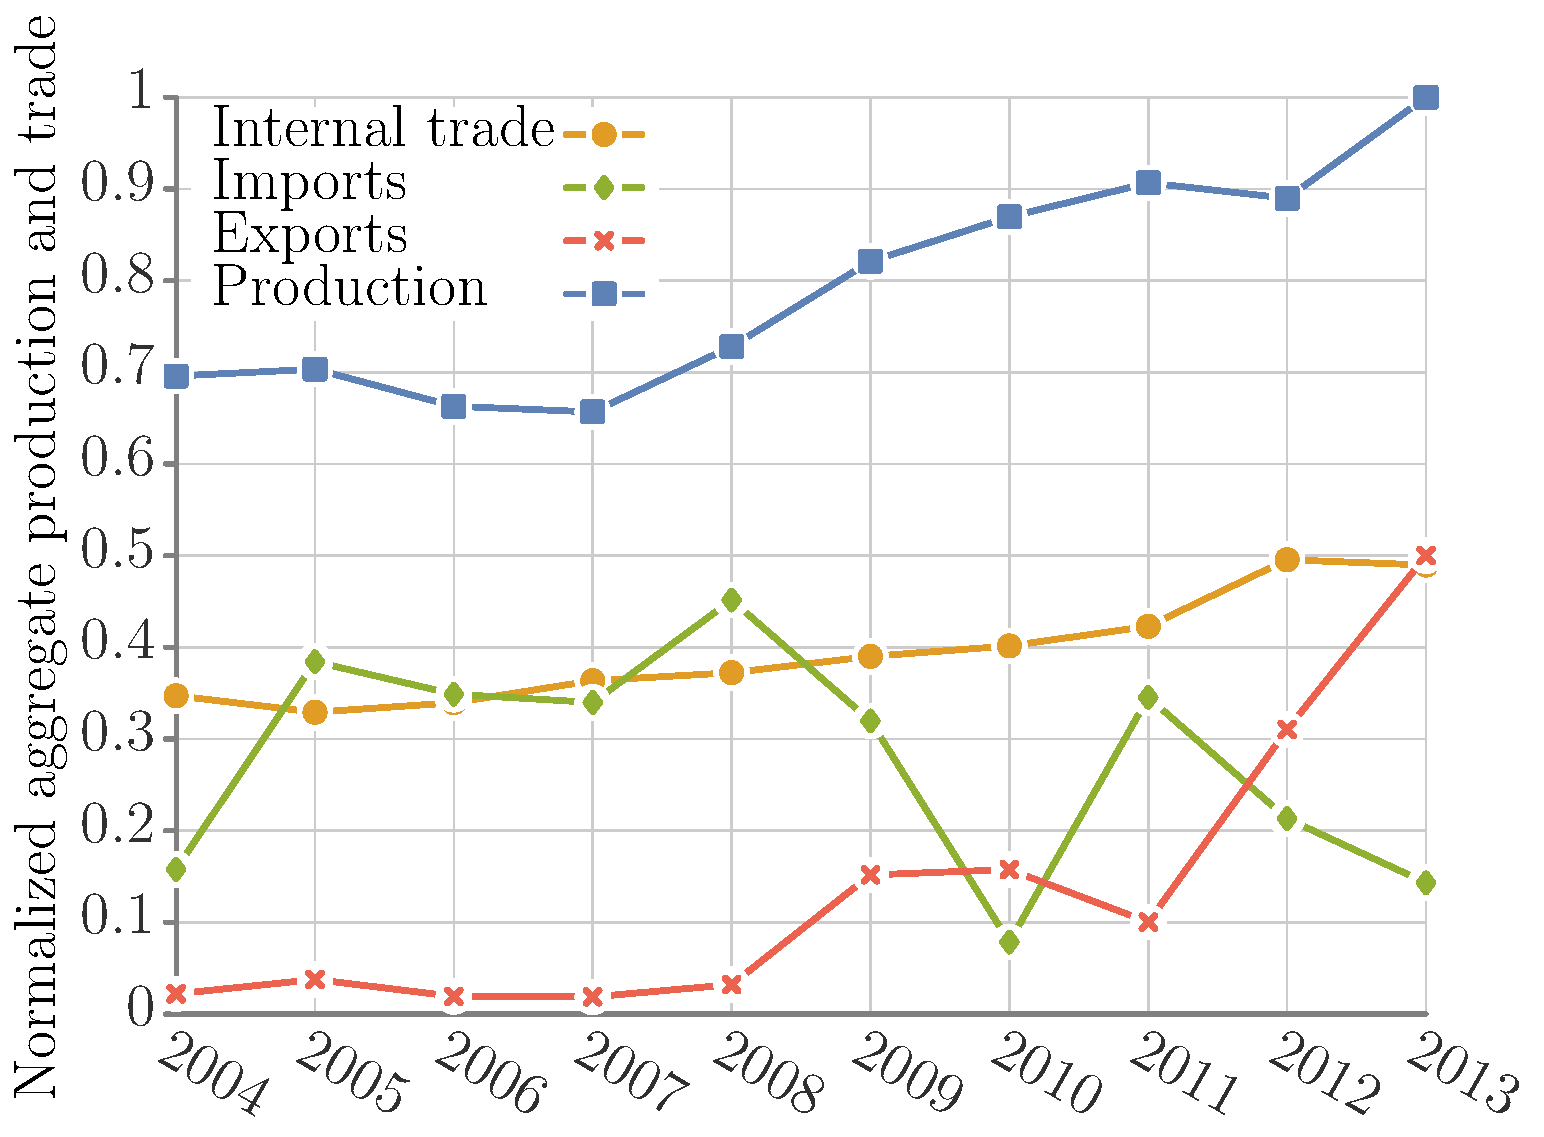
\includegraphics[width=.7\textwidth]
    {../international_trade/results/stat_plots/trends.pdf}
    %{figs/trends.pdf}
\caption{\textbf{General trends of overall production and trade in the
region over a decade based on FAOSTAT 2013.} The total tomato production in
the study region obtained by summing the production for all countries is
plotted for each year between~2004 to~2013 (blue). We computed the total
tomato import volume per year (green) from outside the study region using
FAOSTAT Trade Matrix (Table~\ref{tab:data}). This was obtained by
aggregating imports where the importing country belongs to the study region
and the exporting country is outside the region. Similarly export volume
per year to outside the study region (red) is shown. Finally, the amount of
tomato traded within the study region was obtained by aggregating tomato
trade between countries in the region for each year (orange). In order to
compare these plots, each plot was normalized by dividing by the
corresponding maximum value across all years.
There is a steady
increase in the production and amount of internal trade, with comparable
rate of change for both quantities.  In comparison, the export of tomato to
outside of the focus region (plot ``Exports'') has risen steeply in the
recent years (after 2011), while the imports generally indicate a downward trend (plot
``Imports''). Recent efforts to increase production and trade
infrastructure in these countries support these 
trends~\cite{huong2013,buntong2013,moustier2007}.
Under these circumstances, \tuta{}'s invasion can have a high negative
impact on the economy and livelihood of the people in this region.
\label{fig:trends}} 
%% The filled curves for the three trade plots depict
%% the discrepancy in reporting. For every pair of countries,
%% FAOSTAT Trade Matrix potentially provides two estimates of commodity flow, one by the
%% source country (called ``Import Quantity'') and the other by the
%% destination country (``Export Quantity'').
\end{figure}

\begin{figure}[!ht]
    \centering
\begin{subfigure}[b]{.32\textwidth}
    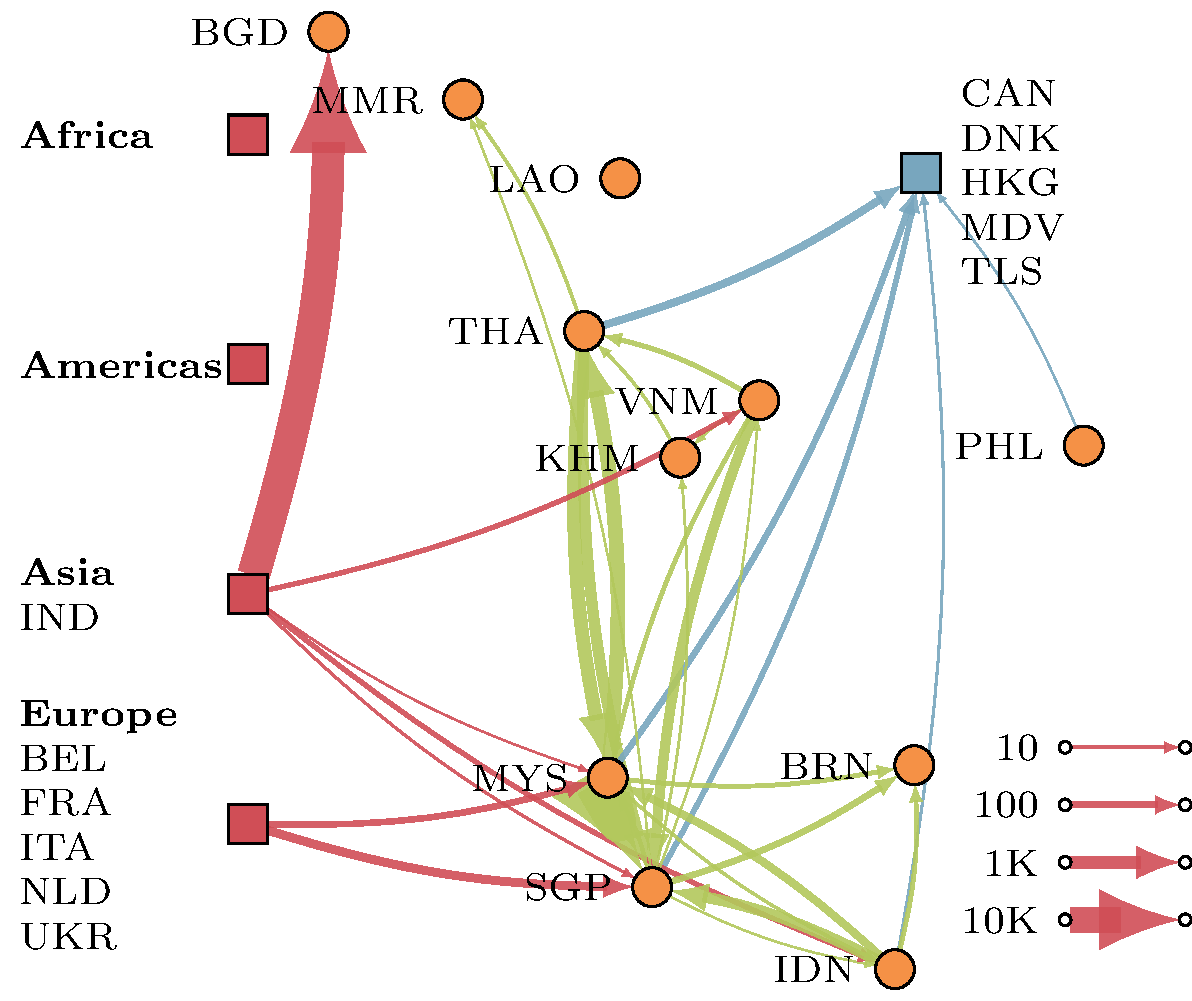
\includegraphics[width=\textwidth]{../international_trade/results/network_plots/sea_2011_tomato.pdf}
    \caption{2011}
\end{subfigure}
    %%
\begin{subfigure}[b]{.32\textwidth}
    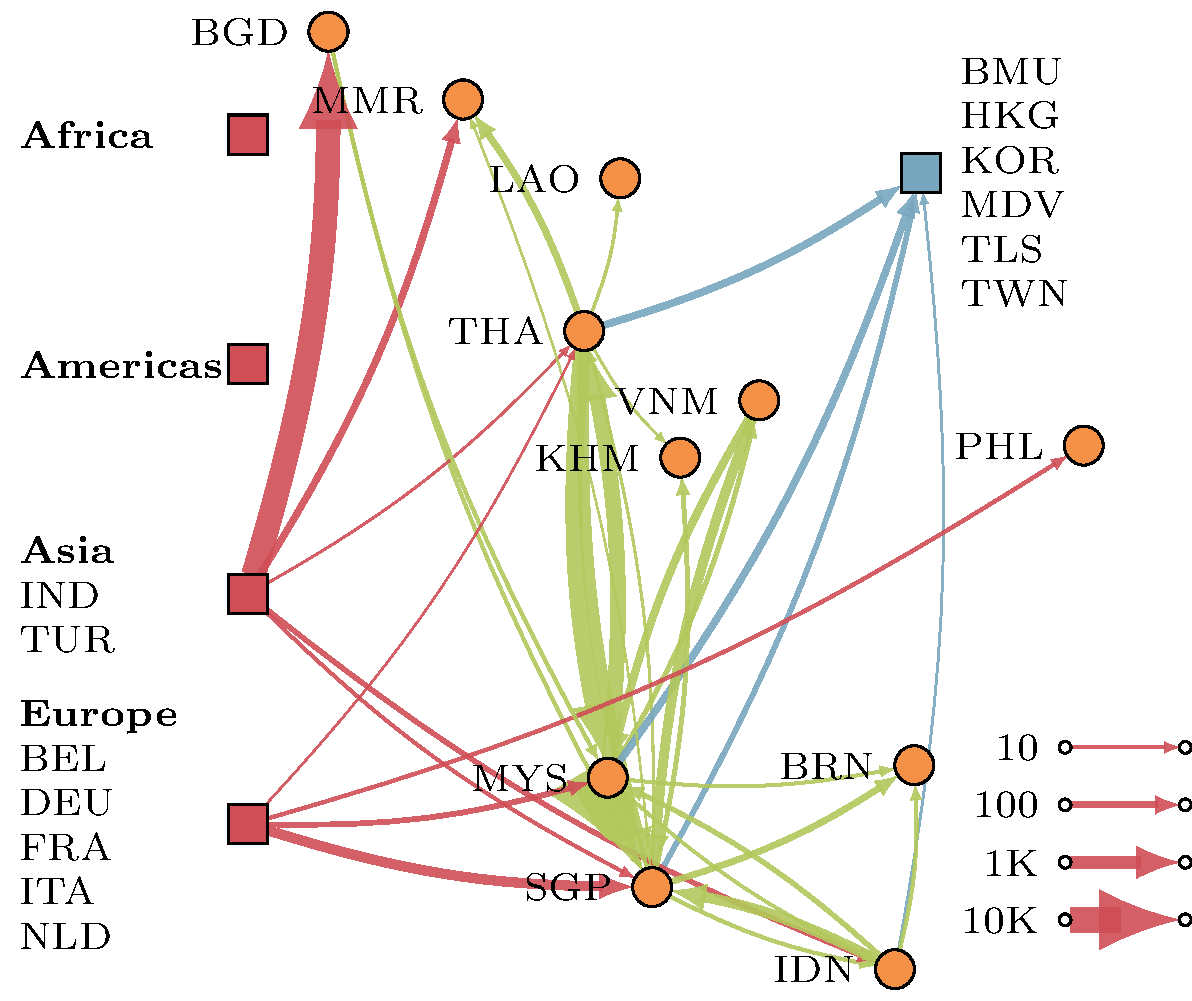
\includegraphics[width=\textwidth]{../international_trade/results/network_plots/sea_2012_tomato.pdf}
    \caption{2012}
\end{subfigure}
    %%
\begin{subfigure}[b]{.32\textwidth}
    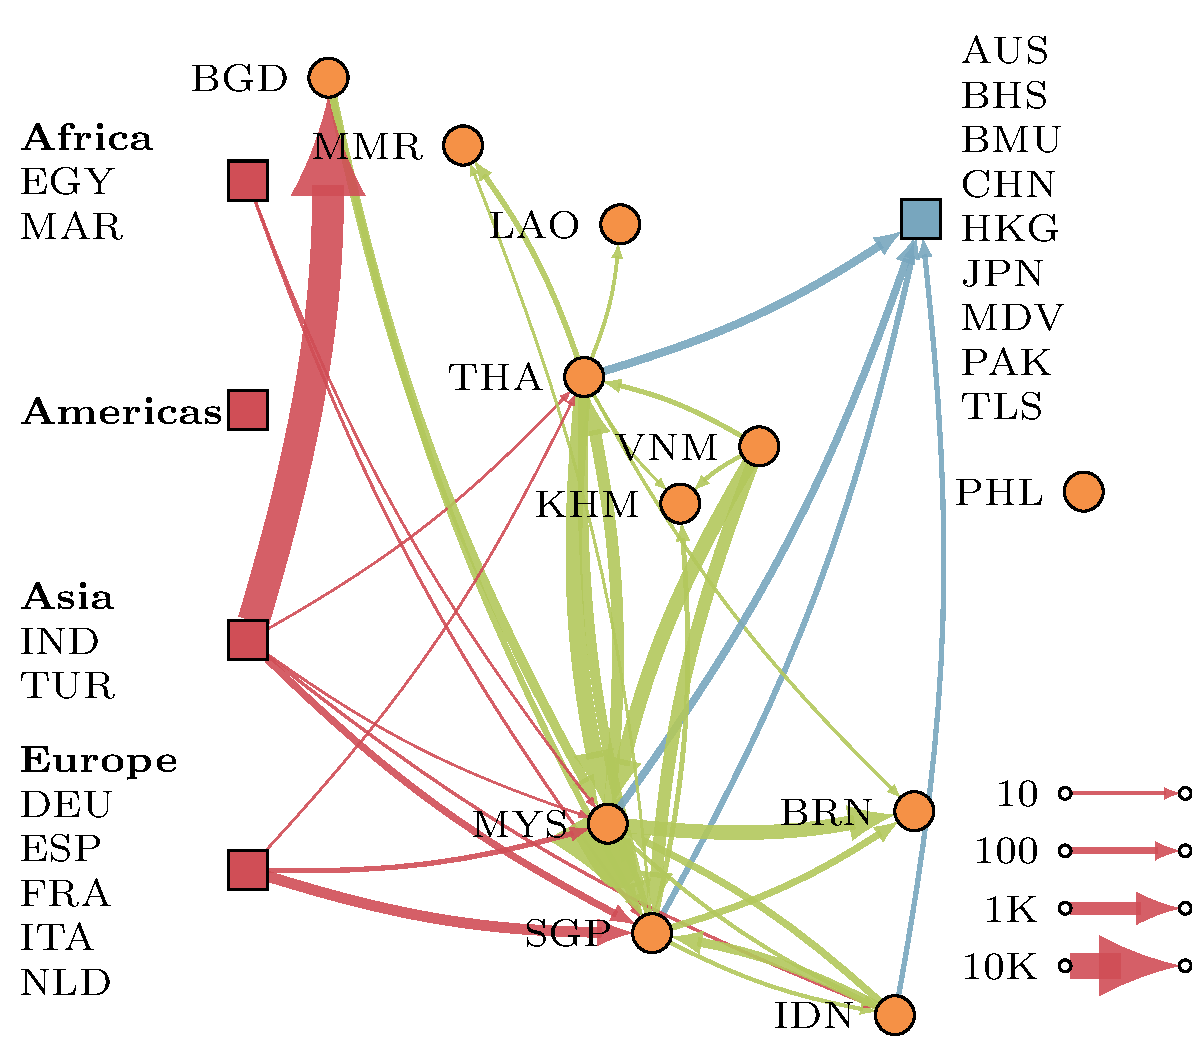
\includegraphics[width=\textwidth]{../international_trade/results/network_plots/sea_2013_tomato.pdf}
    \caption{2013}
\end{subfigure}
    %%
\caption{Evolution of tomato trade network over the years.}
\label{fig:tradeYears}
\end{figure}
%%
%%
%% \begin{figure}[!ht]
%% \centering
%% \begin{subfigure}[b]{.24\textwidth}
%% 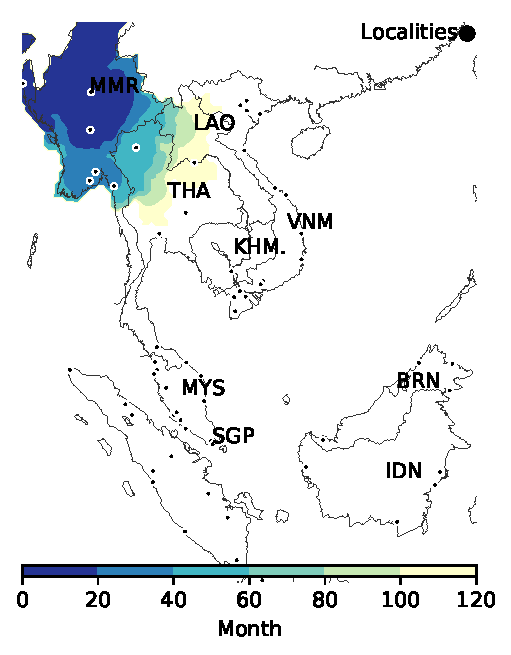
\includegraphics[width=\textwidth]{../cellular_automata/results/contour/MSA_model-A_m1_l1.pdf}
%% \caption{$\mooreRange=1$, $\ell=1$}
%% \end{subfigure}
%% %%
%% \begin{subfigure}[b]{.24\textwidth}
%% 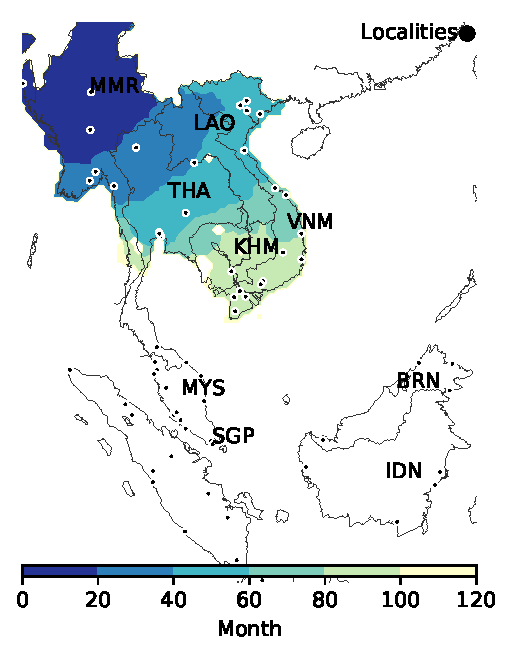
\includegraphics[width=\textwidth]{../cellular_automata/results/contour/MSA_model-A_m2_l1.pdf}
%% \caption{$\mooreRange=2$, $\ell=1$}
%% \end{subfigure}
%% %%
%% \begin{subfigure}[b]{.24\textwidth}
%% 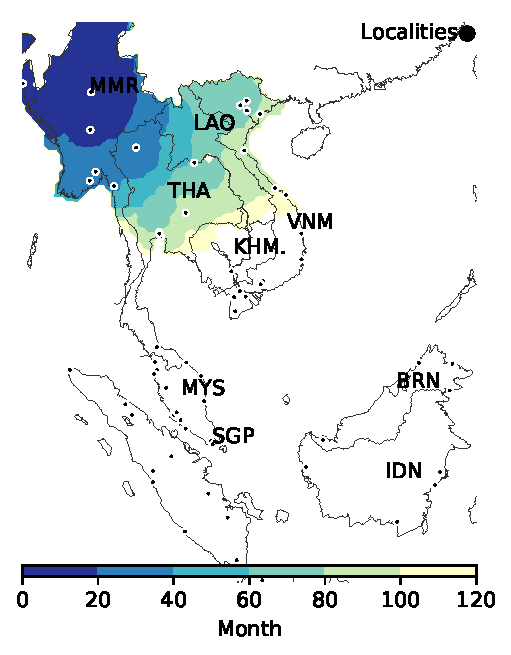
\includegraphics[width=\textwidth]{../cellular_automata/results/contour/MSA_model-A_m2_l2.pdf}
%% \caption{$\mooreRange=2$, $\ell=2$}
%% \end{subfigure}
%% %%
%% \begin{subfigure}[b]{.24\textwidth}
%% 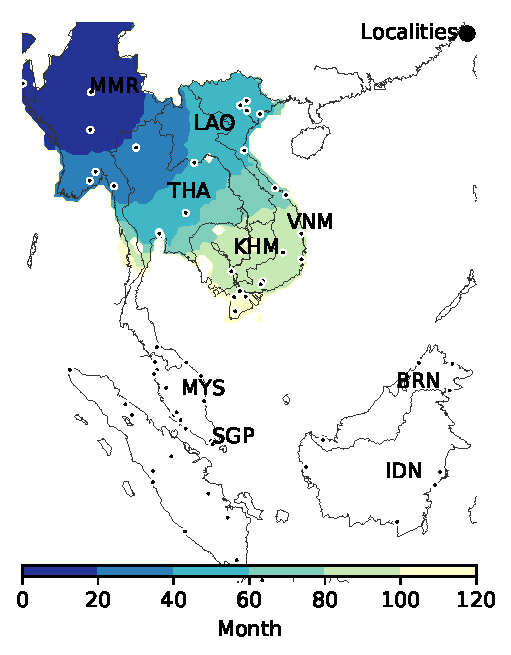
\includegraphics[width=\textwidth]{../cellular_automata/results/contour/MSA_model-A_m3_l3.pdf}
%% \caption{$\mooreRange=3$, $\ell=3$}
%% \end{subfigure}
%% %%
%% \caption{Model A: The projected spread based on selected models. We observe
%% difference in rate of spread for different $(\mooreRange,\ell)$ values.
%% However, the spread pattern itself is similar. The spread is more eastward
%% than southward.}
%% \end{figure}
%%
%% \begin{figure}[!ht]
%% \centering
%% \begin{subfigure}[b]{.24\textwidth}
%% \includegraphics[width=\textwidth]{../cellular_automata/results/contour/MSA_model-B_m1_l2.pdf}
%% \caption{$\mooreRange=1$, $\ell=2$}
%% \end{subfigure}
%% %%
%% \begin{subfigure}[b]{.24\textwidth}
%% \includegraphics[width=\textwidth]{../cellular_automata/results/contour/MSA_model-B_m1_l3.pdf}
%% \caption{$\mooreRange=1$, $\ell=3$}
%% \end{subfigure}
%% %%
%% \begin{subfigure}[b]{.24\textwidth}
%% \includegraphics[width=\textwidth]{../cellular_automata/results/contour/MSA_model-B_m2_l3.pdf}
%% \caption{$\mooreRange=2$, $\ell=3$}
%% \end{subfigure}
%% %%
%% \begin{subfigure}[b]{.24\textwidth}
%% \includegraphics[width=\textwidth]{../cellular_automata/results/contour/MSA_model-B_m3_l3.pdf}
%% \caption{$\mooreRange=3$, $\ell=3$}
%% \end{subfigure}
%% %%
%% \begin{subfigure}[b]{.24\textwidth}
%% \includegraphics[width=\textwidth]{../cellular_automata/results/contour/MSA_50p_model-B_m1_l2.pdf}
%% \caption{50\% increase, $\mooreRange=1$, $\ell=2$}
%% \end{subfigure}
%% %%
%% \begin{subfigure}[b]{.24\textwidth}
%% \includegraphics[width=\textwidth]{../cellular_automata/results/contour/MSA_50p_model-B_m1_l3.pdf}
%% \caption{50\% increase, $\mooreRange=1$, $\ell=3$}
%% \end{subfigure}
%% %%
%% \begin{subfigure}[b]{.24\textwidth}
%% \includegraphics[width=\textwidth]{../cellular_automata/results/contour/MSA_50p_model-B_m2_l3.pdf}
%% \caption{50\% increase, $\mooreRange=2$, $\ell=3$}
%% \end{subfigure}
%% %%
%% \begin{subfigure}[b]{.24\textwidth}
%% \includegraphics[width=\textwidth]{../cellular_automata/results/contour/MSA_50p_model-B_m3_l3.pdf}
%% \caption{50\% increase, $\mooreRange=3$, $\ell=3$}
%% \end{subfigure}
%% %%
%% \caption{Model B: The projected spread based on selected models. As in
%% Model A, we observe difference in rate of spread for different
%% $(\mooreRange,\ell)$ values.  However, again, the spread patterns are
%% similar, but different form that of Model A instances; the spread is more
%% southward than eastward.}
%% \end{figure}
%%
\begin{figure}[!ht]
\begin{subfigure}[b]{.28\textwidth}
\includegraphics[width=\textwidth]{../cellular_automata/results/contour/BD_model-B_precip1_m1_l3.pdf}
\caption{Bangladesh: without intervention\label{fig:bgdBContour}}
\end{subfigure}
\begin{subfigure}[b]{.28\textwidth}
\includegraphics[width=\textwidth]{../cellular_automata/results/contour/TH_model-B_precip1_m1_l3.pdf}
\caption{Thailand: without intervention\label{fig:thaBContour}}
\end{subfigure}
\begin{subfigure}[b]{.28\textwidth}
\includegraphics[width=\textwidth]{../cellular_automata/results/contour/VN_model-B_precip1_m1_l3.pdf}
\caption{Vietnam: without intervention\label{fig:vnmBContour}}
\end{subfigure}
%%
\begin{subfigure}[b]{.28\textwidth}
\includegraphics[width=\textwidth]{../cellular_automata/results/contour/BD_model-B_precip1-out-100_m1_l3.pdf}
\caption{Bangladesh: with intervention (100\%)\label{fig:bgdBContourInt}}
\end{subfigure}
\begin{subfigure}[b]{.28\textwidth}
\includegraphics[width=\textwidth]{../cellular_automata/results/contour/TH_model-B_precip1-out-100_m1_l3.pdf}
\caption{Thailand: with intervention (100\%)\label{fig:thaBContourInt}}
\end{subfigure}
\begin{subfigure}[b]{.28\textwidth}
\includegraphics[width=\textwidth]{../cellular_automata/results/contour/VN_model-B_precip1-out-100_m1_l3.pdf}
\caption{Vietnam: with intervention\label{fig:vnmBContourInt}}
\end{subfigure}
%%
\begin{subfigure}[b]{.32\textwidth}
\includegraphics[width=\textwidth]{../cellular_automata/results/dist_inf_plots/BD_dist_prob_B_box.pdf}
\caption{Bangladesh: spread intensity and distance with respect to origin\label{fig:bgdBContourBox}}
\end{subfigure}
\begin{subfigure}[b]{.32\textwidth}
\includegraphics[width=\textwidth]{../cellular_automata/results/dist_inf_plots/TH_dist_prob_B_box.pdf}
\caption{Thailand: spread intensity and distance with respect to origin\label{fig:thaBContourBox}}
\end{subfigure}
\begin{subfigure}[b]{.32\textwidth}
\includegraphics[width=\textwidth]{../cellular_automata/results/dist_inf_plots/VN_dist_prob_B_box.pdf}
\caption{Vietnam: spread intensity and distance with respect to
origin\label{fig:vnmBContourBox}}
\end{subfigure}
\caption{\textbf{Interventions.} This is a continuation of
    Figure~\ref{M:fig:intervene} from the main document. The results of intervention for three
    other countries are shown. \label{fig:intervene}}
\end{figure}


%%
\section{Cellular automata model from Guimapi~et~al}
\label{sec:guimapi}
Guimapi~et~al.~\cite{guimapi2016modeling} use a cellular automata approach
to model the spread of \tuta{} through the study region of Africa, Spain, and Portugal. 
Here, we implemented and applied the model to study the spread in the focus
region.
%%
\paragraph{Methodology.}
Each cell in the automata is of size $25\mathrm{km}\times25\mathrm{km}$ induced by a
grid overlayed on the study region. Both square and hexagonal cell
configurations are considered, but square cells (Moore neighborhood) were
chosen in order to cover a larger area per cell.
Each cell can be in one of three states: S, E and I with very similar
definitions as in our model.
The spread is modeled as follows:
For an infected cell to spread to another, each cell within its moore
neighborhood of respective distance is considered in each time step (one month). If this neighbor cell is
suitable, it will change states. The suitability of a cell for pest
establishment depends on temperature, humidity, NDVI, and tomato production
in that cell at the given time step.
%\aacomment{Need to say what each time step corresponds to} 
Two Moore neighborhoods were
considered, one with a range of 50 km and another with a range of 75 km.
%\aacomment{I don't think they claim that theirs is a natural spread model.
%Correct me if I am wrong.}

Given a cell within the Moore neighborhood of an infected cell, its state
in the next time step depends on the following rules.
\begin{itemize} 
\item If NDVI $\ge$ NDVI threshold 1, then state becomes "Exposed".
\item If NDVI $\ge$ NDVI threshold 1 and temperature $>=$ temperature threshold and humidity $>=$ humidity threshold, then state becomes "Invaded".
\item If NDVI $\ge$ NDVI threshold 2 and tomato production high or very high, then state becomes "Invaded".
\item Otherwise the state remains unchanged
\end{itemize}

%\aacomment{refer to figure in paper, remove figure from here}.
%\noindent
%% Figure 2 in \cite{guimapi2016modeling} gives these rules for changing states.
%\begin{figure}[ht]
%        \centering
%        \includegraphics[width=\textwidth]{figs/Guimapi_fig.png}
%        \caption{Rules for changing states}
%        \label{Guimapi_rules}
%\end{figure}
Temperature, humidity, and NDVI data is at the level of the cell, while
production data is at the country-level. The temperature threshold is 22
degrees Celsius and humidity threshold is 55\%. The NDVI threshold 1 is
0.1, and threshold 2 is 0.3. The production yield threshold is 10
tons/hectare to be considered high or very high. Thus if a cell is within a
country with high or very high yield, that cell would be classified at high
or very high yield.
\paragraph{Results.}
We applied the seeding scenarios described in Table~\ref{tab:seeds}. Each
scenario was simulated with Moore neighborhoods of~2 and~3.  The results
are shown in Figure~\ref{fig:baselineMyanmar}.  The model predicts a rapid
radial spread in this region as vegetation and temperature are generally
favorable throughout this region.  The tomato production yield in each
country in the focus region is in the high or very high categories, and
thus did not limit the spread.  Generally, the predicted range expansion is
much faster compared to our models, particularly in the case where Moore
range is~3.

%% The results from this study was that with seeding in Spain, Tuta would
%% spread radially. This is due to taking into account only short distance
%% spread, and the fact that no area was unsuitable year-round. They
%% introduced parameters in stages, first considering only NDVI, and assuming
%% that temperature and humidity reached the thresholds. In this scenario,
%% Tuta spread to every region of Africa, excluding Madagascar, in 6 years.
%% When including temperature as a parameter as well, Tuta spreads to all of
%% Africa, excluding Madagascar, in 9 years. When taking into account NDVI,
%% temperature, and humidity as described above, every region of Africa is
%% invaded in 9 years (excluding Madagascar), except for regions in the Sahara
%% desert, which is in the exposed state.


%\aacomment{This part will be moved to results}
%\aacomment{Need to describe each scenario: how the initial seeds were
%decided, the basis for choosing them. I think it is a good idea to also
%name them (Scenario A, B, C, etc.)}


%% We used the CA model by Guimapi~et.~al.~\cite{guimapi2016modeling} as a
%% baseline for our study. We will test three scenarios using this model in Southeast Asia. Scenario A seeds the region of Chin in northeast Myanmar. This region represents a possible pathway of \tuta{} should it spread radially through the border with Bangladesh. Scenario B seeds the region of Johor in Malaysia - including Singapore. This region contains major ports in Malaysia including Tanjung Pelepas \cite{khalid2005}, and Singapore is also a major trading hub for Bangladesh. Scenario C seeds the region of Putrajaya, which is the region which includes the largest port in Malaysia \cite{khalid2005}. Scenario D seeds the region of Penang, which is also a major port \cite{khalid2005}. Scenario E seeds Sarawak which is one of the Malaysia districts not in the mainland. This district contains another major port: Bintulu \cite{khalid2005}. Each scenario is simulated with Moore neighborhoods of 2 and 3, and follow the rules as in \cite{guimapi2016modeling}. Our grid resolution is 0.25x0.25 degrees. This corresponds to about 27.75 km at the equator. Thus one cell will be roughly 25x25 km as in above. We consider Moore neighborhoods of 2 and 3 to reflect 50 - 75 km range. For NDVI data, our resolution is small, so we choose the maximum NDVI for a grid cell.\\


\begin{figure}[ht]
\begin{subfigure}[b]{.47\textwidth}
\centering
\includegraphics[width=\textwidth]{figs/plot_Myanmar2.pdf}
\caption{Moore neighborhood of 2}
\end{subfigure}
\begin{subfigure}[b]{.47\textwidth}
\centering
\includegraphics[width=\textwidth]{figs/plot_Myanmar3.pdf}
\caption{Moore neighborhood of 3, baseline model}
\end{subfigure}
\caption{Guimapi~et~al.~\cite{guimapi2016modeling} model results: 
Here the region of Chin in northeast Myanmar was seeded.
    \label{fig:baselineMyanmar}}
\end{figure}

\bibliographystyle{plain}
\bibliography{refs}
\end{document}

pending:
- Production validation figures: keys need to be corrected
- seeding scenarios to be explained better
- calibration phase needs to be explained
